\documentclass{vkr}
\usepackage[english, russian]{babel} % переносы
\usepackage{graphicx} % для вставки картинок
\graphicspath{{images/}} % путь к изображениям
\usepackage[hidelinks]{hyperref}
\usepackage{float} % определяет метод H для рисунка с переносом на следующую страницу, ели не помещается
\usepackage{pdflscape}
\addto{\captionsrussian}{\renewcommand{\refname}{СПИСОК ИСПОЛЬЗОВАННЫХ ИСТОЧНИКОВ}}
\usepackage{xltabular} % для вставки таблиц
\usepackage{makecell}
\renewcommand\theadfont{} % шрифт в /thead
\usepackage{array} % для определения новых типов столбцов таблиц
\newcolumntype{T}{>{\centering\arraybackslash}X} % новый тип столбца T - автоматическая ширина столбца с выравниванием по центру
\newcolumntype{R}{>{\raggedleft\arraybackslash}X} % новый тип столбца R - автоматическая ширина столбца с выравниванием по правому краю
\newcolumntype{C}[1]{>{\centering\let\newline\\\arraybackslash\hspace{0pt}}m{#1}} % новый тип столбца C - фиксированная ширина столбца с выравниванием по центру
\newcolumntype{r}[1]{>{\raggedleft\arraybackslash}p{#1}} % новый тип столбца r - фиксированная ширина столбца с выравниванием по правому краю
\newcommand{\centrow}{\centering\arraybackslash} % командой \centrow можно центрировать одну ячейку (заголовок) в столбце типа X или p, оставив в оcтальных ячейках другой тип выравнивания
\newcommand{\finishhead}{\endhead\hline\endlastfoot}
\newcommand{\continuecaption}[1]{\captionsetup{labelformat=empty} \caption[]{#1}\\ \hline }
\usepackage{etoolbox}
\AtBeginEnvironment{xltabular}{\refstepcounter{tablecnt}} % подсчет таблиц xltabular, обычные таблицы подсчитываются в классе

\usepackage[tableposition=top]{caption} % подпись таблицы вверху
\captionsetup{strut=off}
\setlength{\intextsep}{0pt} % Vertical space above & below [h] floats
\setlength{\textfloatsep}{0pt} % Vertical space below (above) [t] ([b]) floats
\DeclareCaptionLabelFormat{gostfigure}{Рисунок #2} %подпись рисунка
\DeclareCaptionLabelFormat{gosttable}{Таблица #2} %подпись таблицы
\DeclareCaptionLabelSeparator{gost}{~--~} %разделитель в рисунках и таблицах
\captionsetup{labelsep=gost}
\captionsetup[figure]{aboveskip=10pt,belowskip=4mm,justification=centering,labelformat=gostfigure} % настройка подписи рисунка
\captionsetup[table]{font={stretch=1.41},skip=0pt,belowskip=0pt,aboveskip=8.5pt,singlelinecheck=off,labelformat=gosttable} % настройка подписи таблицы

\setlength{\LTpre}{8mm} % отступ сверху таблицы
\setlength{\LTpost}{6mm} % отступ снизу таблицы

\usepackage{enumitem}
\setlist{nolistsep,wide=\parindent,itemindent=*} % отступы вокруг списков, выравнивание с учетом разделителя

\usepackage{color} %% это для отображения цвета в коде
\usepackage{listings} %% листинги кода
\setmonofont[Scale=0.7]{Verdana} % моноширный шрифт для листинга

\definecolor{codegreen}{rgb}{0,0.6,0}
\definecolor{codegray}{rgb}{0.5,0.5,0.5}
\definecolor{codepurple}{rgb}{0.58,0,0.82}

\lstset{ %
language=C,                 % выбор языка для подсветки (здесь это С)
numbers=left,               % где поставить нумерацию строк (слева\справа)
numberstyle=\tiny,           % размер шрифта для номеров строк
stepnumber=1,                   % размер шага между двумя номерами строк
numbersep=5pt,                % как далеко отстоят номера строк от подсвечиваемого кода
commentstyle=\color{codegreen},
keywordstyle=\color{magenta},
numberstyle=\tiny\color{codegray},
stringstyle=\color{codepurple},
basicstyle=\linespread{0.95}\ttfamily,
backgroundcolor=\color{white}, % цвет фона подсветки - используем \usepackage{color}
showspaces=false,            % показывать или нет пробелы специальными отступами
showstringspaces=false,      % показывать или нет пробелы в строках
showtabs=false,             % показывать или нет табуляцию в строках
frame=single,              % рисовать рамку вокруг кода
tabsize=2,                 % размер табуляции по умолчанию равен 2 пробелам
captionpos=t,              % позиция заголовка вверху [t] или внизу [b] 
breaklines=true,           % автоматически переносить строки (да\нет)
breakatwhitespace=false, % переносить строки только если есть пробел
escapeinside={\%*}{*)}   % если нужно добавить комментарии в коде
}

\makeatletter % чтобы допускались русские комментарии в листингах
\lst@InputCatcodes
\def\lst@DefEC{%
 \lst@CCECUse \lst@ProcessLetter
  ^^80^^81^^82^^83^^84^^85^^86^^87^^88^^89^^8a^^8b^^8c^^8d^^8e^^8f%
  ^^90^^91^^92^^93^^94^^95^^96^^97^^98^^99^^9a^^9b^^9c^^9d^^9e^^9f%
  ^^a0^^a1^^a2^^a3^^a4^^a5^^a6^^a7^^a8^^a9^^aa^^ab^^ac^^ad^^ae^^af%
  ^^b0^^b1^^b2^^b3^^b4^^b5^^b6^^b7^^b8^^b9^^ba^^bb^^bc^^bd^^be^^bf%
  ^^c0^^c1^^c2^^c3^^c4^^c5^^c6^^c7^^c8^^c9^^ca^^cb^^cc^^cd^^ce^^cf%
  ^^d0^^d1^^d2^^d3^^d4^^d5^^d6^^d7^^d8^^d9^^da^^db^^dc^^dd^^de^^df%
  ^^e0^^e1^^e2^^e3^^e4^^e5^^e6^^e7^^e8^^e9^^ea^^eb^^ec^^ed^^ee^^ef%
  ^^f0^^f1^^f2^^f3^^f4^^f5^^f6^^f7^^f8^^f9^^fa^^fb^^fc^^fd^^fe^^ff%
  ^^^^20ac^^^^0153^^^^0152%
  % Basic Cyrillic alphabet coverage
  ^^^^0410^^^^0411^^^^0412^^^^0413^^^^0414^^^^0415^^^^0416^^^^0417%
  ^^^^0418^^^^0419^^^^041a^^^^041b^^^^041c^^^^041d^^^^041e^^^^041f%
  ^^^^0420^^^^0421^^^^0422^^^^0423^^^^0424^^^^0425^^^^0426^^^^0427%
  ^^^^0428^^^^0429^^^^042a^^^^042b^^^^042c^^^^042d^^^^042e^^^^042f%
  ^^^^0430^^^^0431^^^^0432^^^^0433^^^^0434^^^^0435^^^^0436^^^^0437%
  ^^^^0438^^^^0439^^^^043a^^^^043b^^^^043c^^^^043d^^^^043e^^^^043f%
  ^^^^0440^^^^0441^^^^0442^^^^0443^^^^0444^^^^0445^^^^0446^^^^0447%
  ^^^^0448^^^^0449^^^^044a^^^^044b^^^^044c^^^^044d^^^^044e^^^^044f%
  ^^^^0401^^^^0451%
  %%%
  ^^00}
\lst@RestoreCatcodes
\makeatother


% Режим шаблона (должен быть включен один из трех)
\ВКРtrue
%\Практикаtrue
%\Курсоваяtrue

\newcommand{\Дисциплина}{<<Проектирование и архитектура программных систем>>} % для курсовой
\newcommand{\КодСпециальности}{09.03.04} % Курсовая
\newcommand{\Специальность}{Программная инженерия} % Курсовая
\newcommand{\Тема}{Разработка и реализация веб-сервиса} % ВКР Курсовая
\newcommand{\ТемаВтораяСтрока}{ для прослушивания музыки}
\newcommand{\ГдеПроводитсяПрактика}{Юго-Западном государственном университете} % для практики
\newcommand{\РуководительПрактПредпр}{Куркина А. В.} % для практики
\newcommand{\ДолжнРуководительПрактПредпр}{директор} % для практики
\newcommand{\РуководительПрактУнивер}{Чаплыгин А. А.} % для практики
\newcommand{\ДолжнРуководительПрактУнивер}{к.т.н. доцент} % для практики
\newcommand{\Автор}{Д. С. Пашков}
\newcommand{\АвторРод}{Пашкова Д. С.}
\newcommand{\АвторПолностьюРод}{Пашкова Дмитрия Сергеевича} % для практики
\newcommand{\Шифр}{20-06-0162}
\newcommand{\Курс}{4} % для практики
\newcommand{\Группа}{ПО-01б}
\newcommand{\Руководитель}{Е. А. Петрик} % для ВКР и курсовой
\newcommand{\Нормоконтроль}{А. А. Чаплыгин} % для ВКР
\newcommand{\ЗавКаф}{А. В. Малышев} % для ВКР
\newcommand{\ДатаПриказа}{«04» апреля 2024~г.} % для ВКР
\newcommand{\НомерПриказа}{1616-с} % для ВКР
\newcommand{\СрокПредоставления}{«11» июня 2024~г.} % для ВКР, курсового

\begin{document}
\maketitle
\ifПрактика{}\else{
   \newpage
\begin{center}
\large\textbf{Минобрнауки России}

\large\textbf{Юго-Западный государственный университет}
\vskip 1em
\normalsize{Кафедра программной инженерии}
\vskip 1em
\ifВКР{
        \begin{flushright}
        \begin{tabular}{p{.4\textwidth}}
        \centrow УТВЕРЖДАЮ: \\
        \centrow Заведующий кафедрой \\
        \hrulefill \\
        \setarstrut{\footnotesize}
        \centrow\footnotesize{(подпись, инициалы, фамилия)}\\
        \restorearstrut
        «\underline{\hspace{1cm}}»
        \underline{\hspace{3cm}}
        20\underline{\hspace{1cm}} г.\\
        \end{tabular}
        \end{flushright}
        }\fi
\end{center}
\vspace{1em}
  \begin{center}
  \large
\ifВКР{
ЗАДАНИЕ НА ВЫПУСКНУЮ КВАЛИФИКАЦИОННУЮ РАБОТУ
  ПО ПРОГРАММЕ БАКАЛАВРИАТА}
  \else
ЗАДАНИЕ НА КУРСОВУЮ РАБОТУ (ПРОЕКТ)
\fi
\normalsize
  \end{center}
\vspace{1em}
{\parindent0pt
  Студента \АвторРод, шифр\ \Шифр, группа \Группа
  
1. Тема «\Тема\ \ТемаВтораяСтрока»
\ifВКР{
утверждена приказом ректора ЮЗГУ от \ДатаПриказа\ № \НомерПриказа
}\fi.

2. Срок предоставления работы к защите \СрокПредоставления

3. Исходные данные для создания программной системы:

3.1. Перечень решаемых задач:}

\renewcommand\labelenumi{\theenumi)}

\begin{enumerate}
\item Провести анализ предметной области; определить ключевые особенности предметной области и перспективы программного проекта.
\item Разработать модель данных прграммной системы; определить ключевые сущности; разработать проект базы данных.
\item Спроектировать клиентскую и серверную части программной системы; на основе требований пользователей спроектировать пользовательский интерфейс.
\item Произведсти системное тестирование системы; написать модульные тесты.
\end{enumerate}

{\parindent0pt
  3.2. Входные данные и требуемые результаты для программы:}

\begin{enumerate}
\item Входными данными для программной системы являются: учетные данные пользователей, поисковые запросы, изображения.
\item Выходными данными для программной системы являются: результаты поиска, страницы исполнителей, альбомов, плейлистов и пользователей, аудиопоток.
\end{enumerate}

{\parindent0pt

  4. Содержание работы (по разделам):
  
  4.1. Введение
  
  4.1. Анализ предметной области
  
4.2. Техническое задание: основание для разработки, назначение разработки,
требования к программной системе, требования к оформлению документации.

4.3. Технический проект: общие сведения о программной системе, проект
данных программной системы, проектирование архитектуры программной системы, проектирование пользовательского интерфейса программной системы.

4.4. Рабочий проект: спецификация компонентов и классов программной системы, тестирование программной системы, сборка компонентов программной системы.

4.5. Заключение

4.6. Список использованных источников

5. Перечень графического материала:

\списокПлакатов

\vskip 2em
\begin{tabular}{p{6.8cm}C{3.8cm}C{4.8cm}}
Руководитель \ifВКР{ВКР}\else работы (проекта) \fi & \lhrulefill{\fill} & \fillcenter\Руководитель\\
\setarstrut{\footnotesize}
& \footnotesize{(подпись, дата)} & \footnotesize{(инициалы, фамилия)}\\
\restorearstrut
Задание принял к исполнению & \lhrulefill{\fill} & \fillcenter\Автор\\
\setarstrut{\footnotesize}
& \footnotesize{(подпись, дата)} & \footnotesize{(инициалы, фамилия)}\\
\restorearstrut
\end{tabular}
}

\renewcommand\labelenumi{\theenumi.}

   \abstract{РЕФЕРАТ}

Объем работы равен \formbytotal{lastpage}{страниц}{е}{ам}{ам}. Работа содержит \formbytotal{figurecnt}{иллюстраци}{ю}{и}{й}, \formbytotal{tablecnt}{таблиц}{у}{ы}{}, \arabic{bibcount} библиографических источников и \formbytotal{числоПлакатов}{лист}{}{а}{ов} графического материала. Количество приложений – 2. Графический материал представлен в приложении А. Фрагменты исходного кода представлены в приложении Б.

Перечень ключевых слов: веб-сервис, музыкальное воспроизведение, разработка, программное обеспечение, веб-приложение, пользовательский интерфейс, аудио поток, база данных, музыкальные жанры, авторизация, аутентификация, стриминговая технология, API, диаграмма.

Объектом разработки является веб-сервис для прослушивания музыки.

Целью выпускной квалификационной работы является является разработка и реализация веб-сервиса для прослушивания музыки, который предоставит пользователям  доступ к музыкальному контенту, обеспечит высокое качество звука и предоставит функционал для создания и управления персональными плейлистами.

При разработке приожения были выделены основные сущности предметной области, разработаны классы и методы модулей, обеспечивающие работу с сущностями предметной области, а также корректную работу web-сайта, разработаны страницы, содержащие информацию о исполнителях, их альбомах, плейлистах и пользователях, разработны модули для организации потоковой передачи аудио.

\selectlanguage{english}
\abstract{ABSTRACT}
  

The volume of work is \formbytotal{lastpage}{pages}{}{}. The work contains \formbytotal{figurecnt}{illustrations}{}{}, \formbytotal{tablecnt}{tables}{}{}, \arabic{bibcount} bibliographic sources, and \formbytotal{числоПлакатов}{sheets}{}{}. The number of appendices is 2. The graphical material is presented in Appendix A. Fragments of source code are presented in Appendix B.

List of keywords: web service, music playback, development, software, web application, user interface, audio stream, database, music genres, authentication, authorization, streaming technology, API, diagram.

The object of development is a web service for music playback.

The aim of the graduation project is the development and implementation of a web service for music playback, which will provide users access to music content, ensure high-quality sound, and provide functionality for creating and managing personal playlists.

During the development of the application, the main entities of the subject area were identified, classes and methods of modules were developed to work with the entities of the subject area, as well as to ensure the correct operation of the web site. Pages containing information about artists, their albums, playlists, and users were developed, and modules were developed to organize the streaming of audio.
\selectlanguage{russian}
}\fi
\tableofcontents
\section*{ОБОЗНАЧЕНИЯ И СОКРАЩЕНИЯ}

БД -- база данных.

ИС -- информационная система.

ИТ -- информационные технологии. 

ПО -- программное обеспечение.

РП -- рабочий проект.

СУБД -- система управления базами данных.

ТЗ -- техническое задание.

ТП -- технический проект.

API (Application Programming Interface) --  набор определений и протоколов, которые позволяют различным программным приложениям взаимодействовать друг с другом. 

UML (Unified Modelling Language) -- язык графического описания для объектного моделирования в области разработки программного обеспечения.

\ifПрактика{}\else{\section*{ВВЕДЕНИЕ}
\addcontentsline{toc}{section}{ВВЕДЕНИЕ}

В современном мире веб-сервисы для прослушивания музыки занимают важное место в повседневной жизни людей. С развитием интернета и цифровых технологий потребление музыкального контента значительно изменилось. Пользователи все чаще предпочитают онлайн-сервисы, предоставляющие доступ к обширным библиотекам музыкальных произведений, вместо традиционных методов прослушивания, таких как физические носители или скачивание файлов. Это обусловлено удобством, разнообразием выбора и возможностью прослушивания музыки в любой момент времени и в любом месте.
На момент последних моих данных музыкальные сервисы продолжают развиваться и конкурировать за пользователей с помощью различных инноваций и функций. 
Ведущие платформы, такие как Spotify, Apple Music, YouTube Music и Amazon Music, продолжают оставаться в лидирующих позициях, предлагая широкий выбор музыкального контента и персонализированные рекомендации.
Новые игроки и региональные сервисы также продолжают появляться, усиливая конкуренцию на рынке и способствуя развитию инноваций в музыкальной индустрии. 
Перспективы музыкальных сервисов остаются выскими, поскольку они продолжают приспосабливаться к изменяющимся потребностям пользователей и технологическим инновациям. Развитие их функциональности, контента и доступности на различных устройствах будет ключевым направлением. Инновации в области рекомендательных систем и персонализации контента также сделают сервисы более привлекательными для аудитории. Кроме того, углубление интеграции с другими платформами и сервисами могут стимулировать рост и конкурентоспособность музыкальных сервисов.

\emph{Целью данной работы} является разработка и реализация веб-сервиса для прослушивания музыки, который предоставит пользователям  доступ к музыкальному контенту, обеспечит высокое качество звука и предоставит функционал для создания и управления персональными плейлистами. Для достижения поставленной цели необходимо решить \emph{следующие задачи:}
\begin{itemize}
	\item провести анализ предметной области; определить ключевые особенности предметной области и перспективы программного проекта;
	\item разработать модель данных прграммной системы; определить ключевые сущности; разработать проект базы данных;
	\item спроектировать клиентскую и серверную части программной системы; на основе требований пользователей спроектировать пользовательский интерфейс;
	\item произведсти системное тестирование системы; написать модульные тесты.
\end{itemize}

\emph{Целью данной работы} является разработка и реализация веб-сервиса для прослушивания музыки, который предоставит пользователям доступ к музыкальному контенту, обеспечит высокое качество звука и предоставит функционал для создания и управления персональными плейлистами. Для достижения поставленной цели необходимо решить \emph{следующие задачи:}
\begin{itemize}
	\item провести анализ предметной области; определить ключевые особенности предметной области и перспективы программного проекта;
	\item разработать модель данных программной системы; определить ключевые сущности; разработать проект базы данных;
	\item спроектировать клиентскую и серверную части программной системы; на основе требований пользователей спроектировать пользовательский интерфейс;
	\item произвести системное тестирование системы; написать модульные тесты.
\end{itemize}

\emph{Структура и объем работы.} Отчет включает введение, четыре раздела основной части, заключение, список использованных источников и два приложения. Текст выпускной квалификационной работы занимает \formbytotal{lastpage}{страниц}{у}{ы}{ы}.

\emph{Во введении} определена цель работы, поставлены задачи разработки, описана структура работы и дано краткое содержание каждого раздела.

\emph{В первом разделе} проводится исследование предметной области разрабатываемой системы.

\emph{Во втором разделе} производится формулировка требований, моделирование вариантов использования.

\emph{В третьем разделе} описываются выбранные технические решения и проект данных разрабатываемой системы.

\emph{В четвертом разделе} описываются классы и их методы, использованные при разработке, а также проводится тестирование созданного приложения.

В заключении подведены итоги проделанной работы, полученные в ходе разработки.

В приложении А представлен графический материал.
В приложении Б содержатся фрагменты исходного кода.
}\fi
\section{Анализ предметной области}

\subsection{Понятия и принципы работы музыкальных сервисов}

Музыкальные сервисы — это цифровые платформы, предназначенные для распространения, доступа и управления музыкальным контентом. Они позволяют пользователям слушать музыку в режиме онлайн через потоковую передачу (стриминг) или скачивать треки для офлайн-прослушивания. Эти сервисы стали важной частью современной музыкальной индустрии, обеспечивая легкий доступ к огромному музыкальному каталогу\cite{mus1}.

Центральным компонентом музыкальных сервисов является предоставление аудио конечному пользователю. Это может быть реализовано как загрузка аудиофайла на устройство клиента или как потоковая передача, позволяющая пользователю начинать прослушивание аудио, не дожидаясь конца загрузки. Современные музыкальные сервисы обычно реализуют оба подхода. Также важной частью приложений данной категории является навигация и поиск в музыкальном каталоге. Все треки имеют метаданные для обеспечения структуризации предоставляемых данных. Зачастую музыкальные сервисы реализуют функции, помогающие пользователям самостоятельно реализовывать структуру треков в своей медиатеке. Примером такой функции являются "лайки" - отметки, которые пользователи могут ставить на треки. Затем отмеченные треки могут быть получены пользователем. Также распространена структуризация с помощью плейлистов. Плейлист — это упорядоченный список музыкальных треков, составленный на основе определённых критериев или предпочтений. Плейлисты могут быть созданы пользователями для личного использования, кураторами для общественного вещания или автоматически сгенерированы музыкальными сервисами на основе алгоритмов анализа предпочтений слушателей. Поиск в каталоге осуществляется по названиям треков, исполнителей, альбомов и плейлистов. Музыкальные сервисы могут содержать социальные функции, например комментарии для альбомов или возможность поделиться плейлистом с другим пользователем системы или в социальных сетях. 

Сравнение музыкальных веб-приложений с традиционными способами доступа к музыке, такими как покупка компакт-дисков, выявляет ряд преимуществ и недостатков. Одним из ключевых преимуществ является удобство: пользователи могут получать доступ к миллионам треков из любой точки мира, где есть доступ в интернет. Это также экономически выгодно, так как пользователи платят за подписку, а не за каждый трек или альбом. Однако это влечёт за собой потенциальные недостатки, такие как зависимость от стабильного интернет-соединения и возможные ограничения на доступ к определённым трекам или альбомам в зависимости от географического местоположения или условий лицензионных соглашений.

\subsection{История развития цифрового аудио и музыкальных сервисов}

История развития музыкальных сервисов охватывает переход от физических носителей к цифровой дистрибуции музыки, что существенно изменило взаимодействие пользователей с музыкальным контентом. Изначально музыка распространялась через такие физические носители, как виниловые пластинки, кассеты и компакт-диски, которые требовали физического владения и использования специального оборудования для воспроизведения.

С развитием интернет-технологий и повышением скорости интернет-соединений в конце 1990-х — начале 2000-х годов начался переход к цифровому распространению музыки. Первые музыкальные сервисы, такие как Napster, предлагали P2P-платформы для обмена файлами, что вызвало значительные споры в области авторских прав. Это привело к законодательным изменениям и разработке новых моделей лицензирования музыкального контента.

Прорывом в легализации цифровой музыки стал запуск iTunes Store компанией Apple в 2003 году, который предложил модель покупки отдельных музыкальных треков и альбомов. Это послужило основой для развития других музыкальных платформ и укрепления цифровой дистрибуции как доминирующего метода в музыкальной индустрии.

Следующим значительным этапом стало появление сервисов стриминга, таких как Spotify и Pandora, в середине 2000-х. Эти сервисы предложили модель подписки, позволяющую пользователям получать неограниченный доступ к музыкальным библиотекам без необходимости покупки каждого трека. Такая модель предоставила пользователю возможность экспериментировать с разнообразным музыкальным контентом и способствовала росту индивидуализации музыкального опыта через алгоритмы рекомендаций.

Появление музыкальных сервисов с подпиской также привело к изменениям в структуре доходов музыкальной индустрии, где значительная часть доходов стала приходиться на стриминг, а не на продажи физических носителей или цифровых копий. Современные технологии также позволили интегрировать музыкальные сервисы с различными устройствами и платформами, расширяя доступность и функциональность для конечного пользователя.

Таким образом, развитие музыкальных сервисов отражает более широкую тенденцию цифровизации в медиа и культуре, где удобство использования, доступность и персонализация стали ключевыми факторами в определении форматов потребления музыкального контента.

\subsection{Анализ рынка музыкальных сервисов}

В 2015 году стриминговые сервисы впервые стали основным источником дохода для музыкальных лейблов и исполнителей. Согласно данным RIAA, в этом году стриминги составили 34,3\% от общего объема выручки музыкальной индустрии, тогда как доходы от сервисов загрузки музыки, таких как iTunes, достигли 34\%. Продажи музыки на физических носителях принесли 28,8\% дохода.
В последнее время отмечается тенденция к уменьшению рынка компакт-дисков и падению продаж цифровой музыки, в то время как доходы от потоковой трансляции музыки продолжают расти. К 2017 году также значительно увеличилась популярность сервисов с платной подпиской. В 2016 году Россия заняла пятое место по числу подписчиков на «Apple Music» после США, Великобритании, Японии и Канады. По данным IFPI за 2017 год, на первом месте по количеству подписчиков в России находится «Apple Music» с 600 тыс. пользователей, на втором — Яндекс.Музыка с 250 тыс., а на третьем — Google Play Music с 100 тыс. подписчиков (согласно рисунку 3). Эксперты оценивают годовой доход этих сервисов от подписок примерно в 2,4 млрд руб. (34 млн долл.)\cite{mus2}.

Согласно данным от IFPI, организации, представляющей глобальную индустрию звукозаписи, мировой рынок музыки вырос на 7,4\% в 2020 году, увеличиваясь уже шестой год подряд. Глобальный музыкальный отчёт IFPI, опубликованный сегодня, указывает, что общая выручка за 2020 год достигла 21,6 миллиарда долларов США.
Рост был обусловлен музыкальным стримингом, причём особенно значительно увеличились доходы от платных подписок, которые выросли на 18,5\%. К концу 2020 года число платных подписок составило 443 миллиона аккаунтов. Всего доходы от стриминговых сервисов, включая как платные подписки, так и сервисы с рекламной поддержкой, увеличились на 19,9\%, составив 13,4 миллиарда долларов или 62,1\% от всего мирового дохода от звукозаписи. Прирост доходов от стриминга более чем компенсировал падение в других сегментах, включая 4,7\%-ное снижение физических продаж и 10,1\%-ное уменьшение доходов от прав на исполнение, большей частью вызванное пандемией COVID-19\cite{ifpi}.

\subsection{Обзор технологий, используемых в музыкальных сервисах}

В основе музыкальных сервисов лежит клиент-серверная модель, где сервер обрабатывает запросы от клиентов, выполняя функции хранения, поиска и передачи музыкальных треков. 
Серверная часть отвечает за основной функционал приложения. Особенностью музыкальных сервисов является необходимость работы с большим количеством медиафайлов, их количество может составлять десятки миллионов. Для этого требуется использование специальных технологий, таких как распределенные файловые системы, объектные хранилища, сети доставки контента. Серверная сторона часто развертывается на облачных платформах, таких как AWS (Amazon Web Services), Google Cloud или Microsoft Azure, что позволяет масштабировать ресурсы в соответствии с изменяющейся нагрузкой и обеспечивать высокую доступность сервиса.
Конечный пользователь взаимодействует с клиенской частью приложения. В качестве клиентской части используются веб- и мобильные приложения.
Веб-приложения реализуются с использованием таких технологий, как HTML5, CSS3 и JavaScript. В основном используются фронтенд-фреймворки,  такие как React.js, Vue.js или Angular, обеспечивающие создание динамических и адаптивных пользовательских интерфейсов, кроссплатформенную совместимость и оптимизированный пользовательский опыт на различных устройствах. 

Для передачи музыкального контента используются различные протоколы стриминга, такие как HLS (HTTP Live Streaming) и DASH (Dynamic Adaptive Streaming over HTTP). Эти протоколы позволяют эффективно передавать аудио- и видеоконтент через интернет, адаптируя качество потока в зависимости от скорости соединения и возможностей устройства пользователя.

Базы данных играют ключевую роль в управлении музыкальными данными, такими как информация о треках, пользователях, плейлистах и предпочтениях. NoSQL базы данных, такие как MongoDB или Cassandra, часто используются для управления большими объемами структурированных и неструктурированных данных, что позволяет обеспечить высокую производительность и масштабируемость.

Алгоритмы машинного обучения и искусственного интеллекта применяются для анализа пользовательских данных и формирования персонализированных рекомендаций. Системы рекомендаций анализируют предпочтения и поведение пользователей, предлагая им музыкальный контент, который может их заинтересовать.
\section{Техническое задание}
\subsection{Основание для разработки}

Основанием для разработки является задание на выпускную квалификационную работу бакалавра "<Разработка и реализация веб сервиса для прослушивания музыки">.

\subsection{Цель и назначение разработки}

Основной задачей выпускной квалификационной работы является разработка и реализация веб сервиса для прослушивания музыки.

Пользователи должны иметь возможность слушать имеющиеся в каталоге треки, а также отмечать понравившееся треки и добавлять треки в плейлисты.

Задачами данной разработки являются:
\begin{itemize}
\item проектирование серверной части приложения;
\item реализация сервиса музыкального каталога;
\item реализация сервиса управления пользователями;
\item реализация сервиса отметки понравившихся треков;
\item реализация поиска контента;
\item проектирование и реализация клиентской части приложения;
\end{itemize}

\subsection{Требования к программной системе}

\subsubsection{Требования к данным программной системы}

На рисунке \ref{concept_data:image} представлена концептуальная модель данных программной системы в виде UML-диаграммы сущность-связь\cite{uml}.

\begin{figure}[h]
	\center{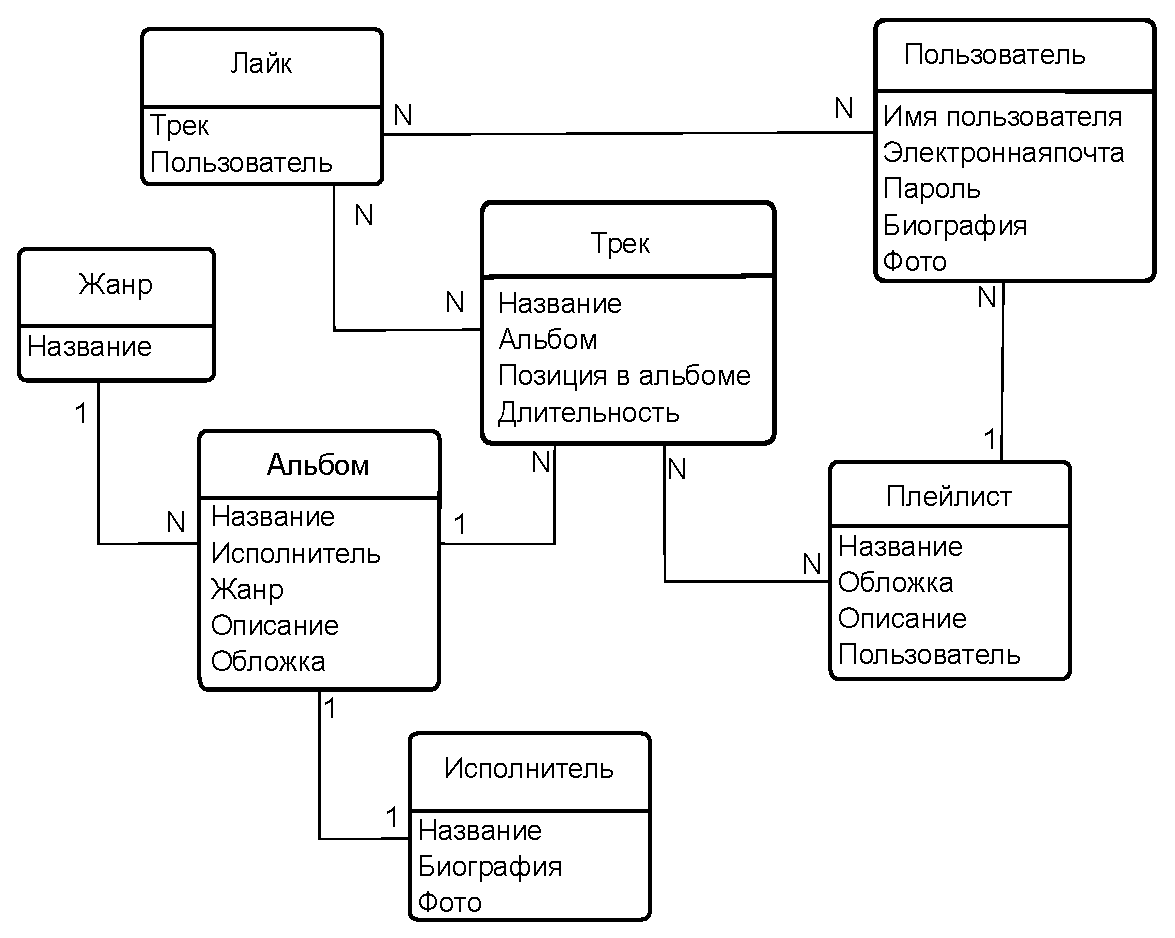
\includegraphics[width=0.7\linewidth]{conc_data}}
	\caption{Концептуальная модель данных}
	\label{concept_data:image}
\end{figure}

\subsubsection{Функиональные требования к программной системе}

К разрабатываемой системе могут получать доступ зарегистрированные и незарегистрированные пользователи. Для незарегистрированных пользователей должна быть реализована функция регистрации в системе.
Для зарегистрированных пользователей должны быть доступны следующие функции:
\begin{enumerate}
	\item Вход по электронной почте и паролю.
	\item Прослушивание выбранных треков.
	\item Поиск по музыкальному каталогу.
	\item Просмотр страниц артистов, альяомов и плейлистов.
	\item Отметка понравившихся треков.
	\item Удаление отметки с отмеченного трека.
	\item Просмотр отмеченных треков.
	\item Создание и удаление созданных пользователем плейлистов.
	\item Добавление и удаление треков из плейлистов.
\end{enumerate}

\paragraph{Моделирование вариантов использования}

Для создаваемого веб-сервиса была разработана модель, позволяющая наглядно демонстрировать различные способы использования сайта. Эта модель способствует физическому проектированию и тщательному анализу связей между элементами системы. В процессе создания диаграммы использования сайта используется стандарт UML для визуального моделирования\cite{uml2}.

Такая диаграмма отражает функциональные задачи, которые система будет выполнять в ходе своей работы, представляя первоначальное концептуальное видение системы на этапах ее проектирования и разработки. Разрабатываемая система изображается через серию сценариев взаимодействия, доступных пользователям или другим внешним агентам. Взаимодействующие с системой агенты могут быть людьми или техническими устройствами, и каждый сценарий описывает серию действий, доступных этим агентам.

После проведения анализа предметной области и функциональных требований были составлены диаграммы прецедентов для неавторизованного и авторизованного пользователей, представленные на рисунках \ref{uc_noauth:image} и \ref{uc_auth:image}
\vspace{1cm}
\begin{figure}[h]
	\center{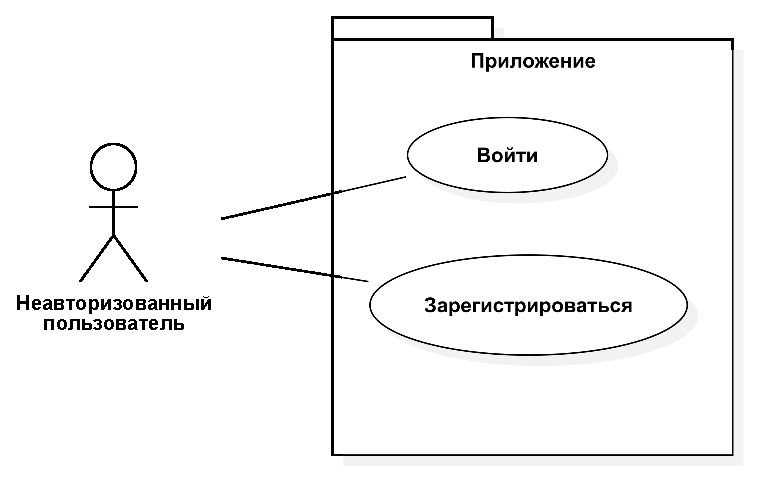
\includegraphics[width=1\linewidth]{uc_noauth}}
	\caption{Диаграмма прецедентов для неавторизованного пользователя}
	\label{uc_noauth:image}
\end{figure}

\begin{figure}[h]
	\center{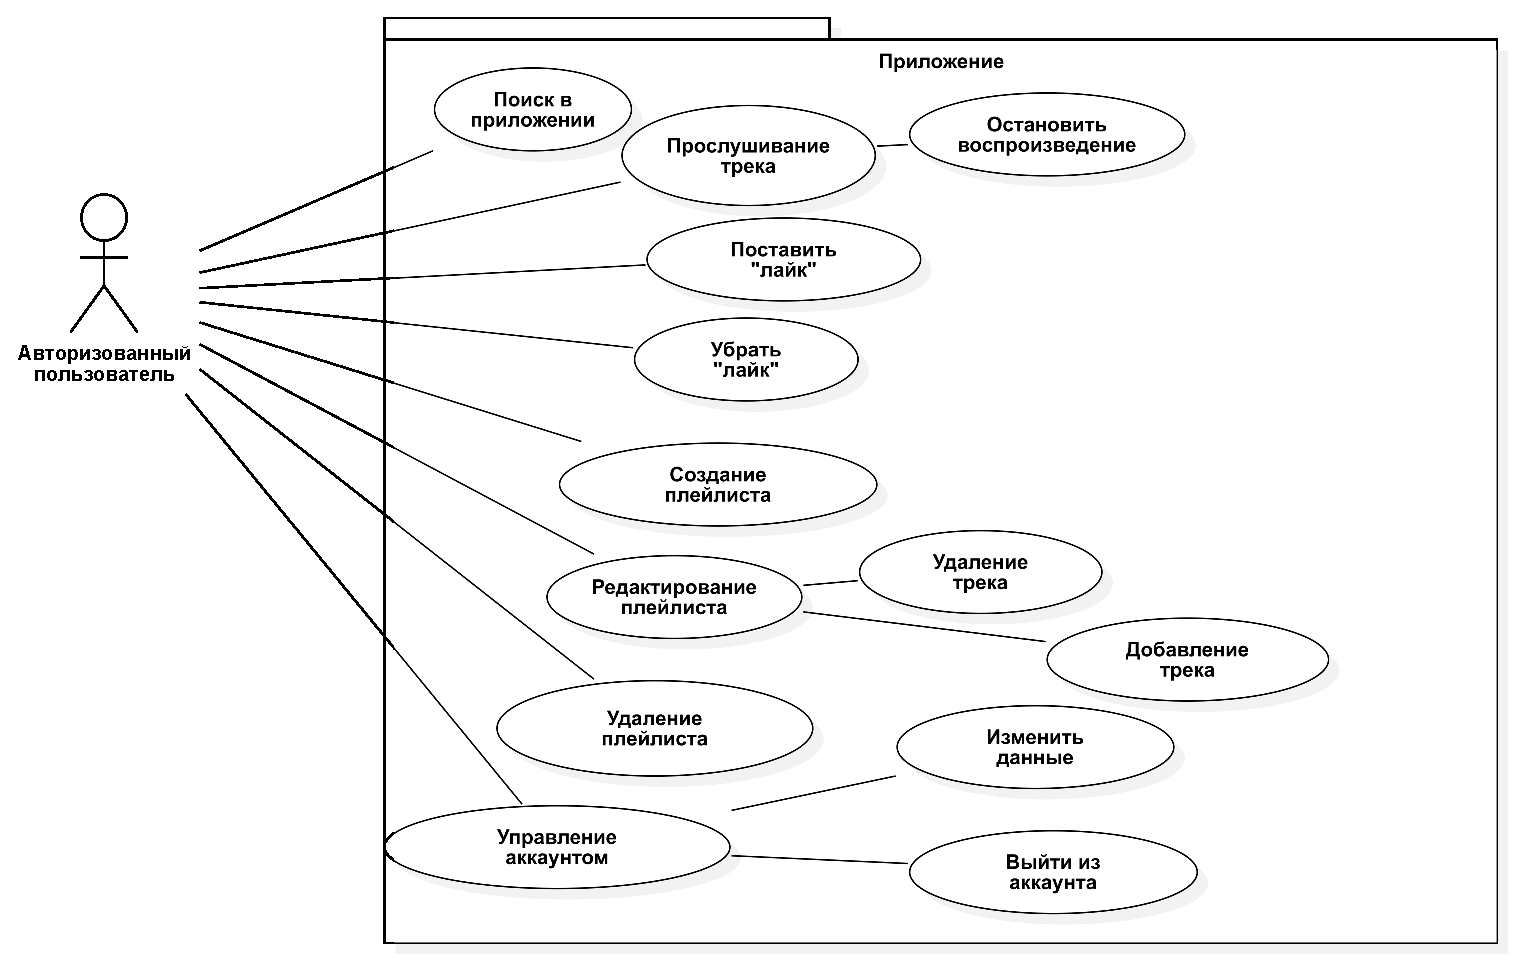
\includegraphics[width=1\linewidth]{uc_auth}}
	\caption{Диаграмма прецедентов для неавторизованного пользователя}
	\label{uc_auth:image}
\end{figure}
\paragraph{Вариант использования "<Регистрация">}

Участники
\begin{itemize}
	\item потенциальный пользователь - человек, желающий создать новую учетную запись.
\end{itemize}

Предусловия:
\begin{itemize}
	\item потенциальный пользователь имеет доступ к интернету;
	\item потенциальный пользователь посещает веб-сайт или открывает приложение, где требуется регистрация.
\end{itemize}

Постусловия:
\begin{itemize}
	\item У пользователя создана учетная запись, он может использовать свой логин и пароль для доступа к сервису;
	\item пользовательская информация сохранена в базе данных сервиса.
\end{itemize}

Основной поток событий:
\begin{enumerate}
	\item Пользователь выбирает опцию "<Регистрация"> на странице.
	\item Пользователь вводит требуемую информацию в форму регистрации: имя пользователя, адрес электронной почты и пароль.
	\item Система проверяет введенные данные на корректность и уникальность.
	\item Система подтверждает успешное создание учетной записи;
	\item Пользователю предоставляется доступ к своему профилю и основным функциям сервиса.
\end{enumerate}

Альтернативные потоки:
\begin{enumerate}
	\item Электронная почта уже используется.
	\begin{enumerate}
		\item Если введенный адрес электронной почты уже зарегистрирован в системе, пользователю предлагается войти в систему.
	\end{enumerate}
	
	\item Ошибка валидации данных.
	\begin{enumerate}
		\item Если данные не проходят валидацию, например, слабый пароль или неправильный формат электронной почты, система выводит соответствующее сообщение об ошибке, и пользователь должен исправить данные.
	\end{enumerate}
\end{enumerate}

\paragraph{Вариант использования "<Вход">}

Участники:
\begin{itemize}
	\item зарегистрированный пользователь - человек, желающий войти в свою учетную запись;
\end{itemize}

Предусловия:
\begin{itemize}
	\item зарегистрированный пользователь имеет активную учетную запись.
\end{itemize}

Постусловия:
\begin{itemize}
	\item пользователь успешно входит в систему;
	\item пользователю предоставляется доступ к своему профилю и персонализированным функциям сервиса.
\end{itemize}

Основной поток событий:
\begin{enumerate}
	\item Пользователь выбирает опцию "<Войти"> на странице.
	\item Пользователь вводит свой адрес электронной почты и пароль в форму входа.
	\item Система проверяет введенные данные на соответствие зарегистрированному профилю.
	\item Система подтверждает успешный вход в систему.
	\item Пользователю открывается доступ к интерфейсу системы.
\end{enumerate}

Альтернативные потоки:
\begin{enumerate}
	\item Неверный логин или пароль.
	\begin{enumerate}
		\item Если данные не соответствуют ни одному из профилей в системе, пользователю предлагается попробовать ввести данные снова.
	\end{enumerate}
\end{enumerate}

\paragraph{Вариант использования "<Поиск">}

Участники:
\begin{itemize}
	\item зарегистрированный пользователь.
\end{itemize}

Предусловия:
\begin{itemize}
	\item зарегистрированный пользователь имеет активную учетную запись и вошел в систему.
\end{itemize}

Постусловия:
\begin{itemize}
	\item пользователь получает результаты, совпадающие с введенной строкой поиска.
\end{itemize}

Основной поток событий:
\begin{enumerate}
	\item Пользователь вводит строку поиска в поле "<Поиск"> на странице.
	\item Система находит запрошенные данные на сервере.
	\item Пользоатель получает список совпадений с введенной строкой.
\end{enumerate}

Альтернативные потоки:
\begin{enumerate}
	\item Отсутствие совпадений.
	\begin{enumerate}
		\item Если система не находит запрошенную информацию, пользователь получает сообщение об отсутствии совпадений.
	\end{enumerate}
\end{enumerate}

\paragraph{Вариант использования "<Прослушать трек">}

Участники:
\begin{itemize}
	\item зарегистрированный пользователь.
\end{itemize}

Предусловия:
\begin{itemize}
	\item зарегистрированный пользователь имеет активную учетную запись и вошел в систему.
\end{itemize}

Постусловия:
\begin{itemize}
	\item трек проигрывается через медиаплеер на устройстве пользователя.
\end{itemize}

Основной поток событий:
\begin{enumerate}
	\item Пользователь выбирает трек для прослушивания, нажимая на сам трек.
	\item Система запускает медиаплеер и начинает воспроизведение выбранного трека.
	\item Во время прослушивания пользователь может управлять воспроизведением.
\end{enumerate}

Альтернативные потоки:
\begin{enumerate}
	\item Прерывание воспроизведения.
	\begin{enumerate}
		\item Пользователь может в любой момент остановить воспроизведение трека, выбрав опцию "<Стоп">.
		\item Система останавливает воспроизведение и ждет других команд.
	\end{enumerate}
\end{enumerate}

\paragraph{Вариант использования "<Поставить "<лайк">">}

Участники:
\begin{itemize}
	\item зарегистрированный пользователь.
\end{itemize}

Предусловия:
\begin{itemize}
	\item зарегистрированный пользователь имеет активную учетную запись и вошел в систему.
\end{itemize}

Постусловия:
\begin{itemize}
	\item трек отмечается иконкой "<лайк">;
	\item система сохраняет "<лайк"> в базу данных.
\end{itemize}

Основной поток событий:
\begin{enumerate}
	\item Пользователь выбирает опцию "<Поставить "<лайк">"> у трека>.
\end{enumerate}

\paragraph{Вариант использования "<Удалить "<лайк">">}

Участники:
\begin{itemize}
	\item зарегистрированный пользователь.
\end{itemize}

Предусловия:
\begin{itemize}
	\item зарегистрированный пользователь имеет активную учетную запись и вошел в систему;
	\item трек отмечен "<лайком">".
\end{itemize}

Постусловия:
\begin{itemize}
	\item у трека удаляется иконка "<лайк">;
	\item система удаляет "<лайк"> из базы данных.
\end{itemize}

Основной поток событий:
\begin{enumerate}
	\item Пользователь выбирает опцию "<Удалить "<лайк">"> у "<лайкнутого">" трека>.
	\item Система удаляет "<лайк">.
\end{enumerate}

\paragraph{Вариант использования "<Создание плейлиста">}

Участники:
\begin{itemize}
	\item зарегистрированный пользователь.
\end{itemize}

Предусловия:
\begin{itemize}
	\item зарегистрированный пользователь имеет активную учетную запись и вошел в систему.
\end{itemize}

Постусловия:
\begin{itemize}
	\item пользователь получает созданный плейлист;
	\item система сохраняет плейлист в базу данных.
\end{itemize}

Основной поток событий:
\begin{enumerate}
	\item Пользователь выбирает опцию "<Создать плейлист">;
	\item Система отображает форму ввода данных.
	\item Пользоатель вводит данные.
	\item \item Система сохраняет плейлист.
\end{enumerate}
	
Альтернативные потоки:
\begin{enumerate}
	\item Отмена создания.
	\begin{enumerate}
		\item Если пользователь передумал создавть плейлист, он нажимает кнопку "<Отмена">.
	\end{enumerate}
\end{enumerate}

\paragraph{Вариант использования "<Редактирование плейлиста">}


Участники:
\begin{itemize}
	\item зарегистрированный пользователь.
\end{itemize}

Предусловия:
\begin{itemize}
	\item зарегистрированный пользователь имеет активную учетную запись и вошел в систему.
\end{itemize}

Постусловия:
\begin{itemize}
	\item пользователь получает измененный плейлист;
	\item система сохраняет изменения плейлиста в базу данных.
\end{itemize}

Основной поток событий:
\begin{enumerate}
	\item Пользователь выбирает опцию "<Изменить плейлист">.
	\item Пользователь выбирает один или несколько треков, которые хочет удалить.
	\item После изменений пользователь выбирает опцию "Сохранить изменения".
\end{enumerate}

Альтернативные потоки:
\begin{enumerate}
	\item Отмена изменений.
	\begin{enumerate}
		\item Если пользователь решил не изменять плейлист, он выбирает опцию "Отменить".
	\end{enumerate}
\end{enumerate}

\paragraph{Вариант использования "<Удаление плейлиста">}

Участники:
\begin{itemize}
	\item зарегистрированный пользователь.
\end{itemize}

Предусловия:
\begin{itemize}
	\item зарегистрированный пользователь имеет активную учетную запись и вошел в систему.
\end{itemize}

Постусловия:
\begin{itemize}
	\item плейлист пропадает из списка плейлистов;
	\item система удаляет плейлист из базы данных.
\end{itemize}

Основной поток событий:
\begin{enumerate}
	\item Пользователь выбирает опцию "<Удалить плейлист">.
	\item Система просит пользователя подтвердить удаление.
	\item После подтверждения пользователя система удаляет плейлист.
\end{enumerate}

Альтернативные потоки:
\begin{enumerate}
	\item Отмена удаления.
	\begin{enumerate}
		\item Если пользователь не удалять плейлист, он выбирает опцию "Отменить" в диалоге подтверждения.
	\end{enumerate}
\end{enumerate}

\paragraph{Вариант использования "<Изменить профиль">}

Участники:
\begin{itemize}
	\item зарегистрированный пользователь.
\end{itemize}

Предусловия:
\begin{itemize}
	\item зарегистрированный пользователь имеет активную учетную запись и вошел в систему.
\end{itemize}

Постусловия:
\begin{itemize}
	\item профиль пользователя обновляется с новыми данными;
	\item изменения сохраняются в базе данных.
\end{itemize}

Основной поток событий:
\begin{enumerate}
	\item Пользователь выбирает опцию "<Изменить профиль">.
	\item Система предоставляет форму для ввода или изменения данных профиля.
	\item Пользователь вносит желаемые изменения в поля формы.
	\item Пользователь подтверждает изменения, выбирая опцию "<Сохранить изменения">.
	\item Система проверяет введенные данные на корректность.
	\item После проверки система обновляет информацию в профиле пользователя.
	\item Система уведомляет пользователя о успешном обновлении профиля.
\end{enumerate}

Альтернативные потоки:
\begin{enumerate}
	\item Отмена изменений.
	\begin{enumerate}
		\item Если пользователь решает не изменять профиль, он может выбрать опцию "Отмена" или закрыть форму изменения профиля.
		\item Система возвращает пользователя на предыдущую страницу без сохранения изменений.
	\end{enumerate}
	\item Ошибка ввода данных.
	\begin{enumerate}
		\item Если введенные данные не соответствуют требованиям (например, имя пользователя слишком длинное или содержит недопустимые символы), система выдает сообщение об ошибке.
		\item Пользователь возвращается к форме для корректировки данных.
	\end{enumerate}
\end{enumerate}

\paragraph{Вариант использования "<Выйти из профиля">}

Участники:
\begin{itemize}
	\item зарегистрированный пользователь.
\end{itemize}

Предусловия:
\begin{itemize}
	\item зарегистрированный пользователь имеет активную учетную запись и вошел в систему.
\end{itemize}

Постусловия:
\begin{itemize}
	\item пользователь выходит из своего профиля;
\end{itemize}

Основной поток событий:
\begin{enumerate}
	\item Пользователь нажимает на опцию "<Выйти"> в панели пользователя.
	\item Система перенаправляет пользователя на страницу входа.
\end{enumerate}


\subsubsection{Требования к пользовательскому интерфейсу}

Для системы дожен быть реализован пользовательский интерфейс на основе веб-технологий\cite{jshtml}\cite{ui2}. Доступ к интерфейсу осуществляется чере веб-браузер. Должна быть предусмотрена возможность адаптации под мобильные экраны.
Интерфейс должен включать в себя:
\begin{itemize}
	\item страницы для авторизации и регистрации;
	\item главная страница для авторизованного пользователя;
	\item поиск по исполнителям, альбомам, трекам, плейлистам;
	\item страница исполнителя;
	\item страница альбома;
	\item страница плейлиста;
	\item плеер для прослушивания треков;
	\item профиль пользователя.
\end{itemize}

\subsubsection{Требования к программному обеспечению}

Для реализации программной системы должны быть использованы
следующие языки программирования:
\begin{itemize}
	\item Java - серверная часть приложеня;
	\item JavaScript - клиентская часть приложения, запросы MongoDB;
	\item SQL  - для запросов в базу данных.
\end{itemize}
Для доступа к клиентской части требуется веб-браузер с поддержкой JavaScript стандарта ECMAScript 2015.

\subsection{Требования к оформлению документации}

Разработка программной документации и программного изделия должна производиться согласно ГОСТ 19.102-77 и ГОСТ 34.601-90. Единая система программной документации.

\section{Технический проект}
\subsection{Общая характеристика организации решения задачи}

Требуется спроектировать и разработать клиентскую(веб-сайт) и серверную часть программно-информационной системы.

Центральной задачей проекта является обеспечение пользователей доступом к библиотеке музыкальных треков и плейлистов через веб-интерфейс. 
В рамках проекта предусмотрена реализация технологий для поддержки непрерывного воспроизведения музыки  Разработка включает в себя создание бэкенд-системы, способной поддерживать стабильную работу сервиса.

\subsection{Обоснование выбора технологии проектирования}

Выбор технологии проектирования является ключевым аспектом в разработке любого программного продукта. Тщательный анализ возможных вариантов и сравнение их характеристик позволили определить оптимальное сочетание технологий, которые обеспечат выполнение всех функциональных требований и гарантируют удобство в дальнейшей поддержке и развитии проекта. 

\subsubsection{Описание используемых технологий и языков программирования}

В процессе разработки backend- и frontend-частей применяются различные технологии и языки программирования, обеспечивающие как простоту разработки, так и производительность конечной системы.

\subsubsection{Язык программирования Java}

Java — строго типизированный объектно-ориентированный язык программирования общего назначения, разработанный компанией Sun Microsystems (в последующем приобретённой компанией Oracle). Разработка ведётся сообществом, организованным через Java Community Process; язык и основные реализующие его технологии распространяются по лицензии GPL. Работает на принципе "<write once, run anywhere"> (WORA), что означает, что скомпилированный Java-код может запускаться на любой платформе без необходимости повторной компиляции. Это достигается за счёт Java Virtual Machine (JVM), которая интерпретирует байт-код Java для выполнения на любой операционной системе\cite{java}. 
В языке реализовано автоматическое управление памятью. Имеет бгатый набор стандартных коллекций: массив, список, стек и т.п.

\subsubsection{Фреймворк Spring}

Spring Framework - универсальный фреймворк для языка Java с открытым исходным кодом. Он предлагает набор модулей для решения типовых задач при разработке, таких как доступ к данным, аутентификация и авторизация, тестирование и другие. В центре фреймворка лежит контейнер инверсии управления, предоставляющий механизмы конфигурирования и управления Java объектами, что позволяет реализовать шаблон "<Внедерние зависимостей">\cite{springboot}.
Основные модули Spring:
\begin{itemize}
	\item Spring Boot - автоконфигурация проектов;
	\item Spring Data - управление данными приложения\cite{persist};
	\item Spring Security - конфигурация авторизации и аутентификации;
	\item Spring Cloud - средства для разработки приложений на основе микросервисной архитектуры\cite{springcloud}.
\end{itemize}

\subsubsection{Язык программирования JavaScript}

JavaScript является высокоуровневым, интерпретируемым языком программирования, который стал стандартом де-факто для веб-разработки на клиентской стороне\cite{js}. Изначально предназначенный для создания интерактивных элементов на веб-страницах, JavaScript со временем значительно расширил свои возможности и теперь используется в разнообразных сферах программирования. JavaScript поддерживает несколько парадигм программирования, что делает его исключительно гибким. 
JavaScript играет важную роль в разработке одностраничных приложений с помощью современных фреймворков и библиотек, таких как Angular, React и Vue.js, которые позволяют создавать интерактивные и масштабируемые пользовательские интерфейсы.

\subsubsection{Фреймворк Vue.js}

Vue.js — это прогрессивный JavaScript фреймворк, предназначенный для создания пользовательских интерфейсов. Основная его особенность заключается в постепенной адаптации: базовый уровень Vue.js фокусируется только на представлении (view layer), что делает его простым в интеграции с другими библиотеками или существующими проектами. Однако при необходимости Vue может легко функционировать и как часть полноценной экосистемы для разработки сложных одностраничных приложений (SPA)\cite{vue}. Фреймворк предоставляет готовые решения для маршрутизации (Vue Router), управления состоянием (Vuex и Pinia), что позволяет легко масштабировать приложение.

\subsection{Архитектура программной системы}

Разрабатываемый программный продукт реализован на основе клиент-серверной архитектуре\cite{arch2}. 
«Клиент — сервер» — это архитектура вычислительных или сетевых систем, где задачи или нагрузка распределяются между сервисами, предоставляемыми серверами, и клиентами, которые эти сервисы используют. Клиент и сервер представляют собой программное обеспечение, обычно расположенное на разных устройствах и взаимодействующее через сеть с использованием сетевых протоколов, хотя они могут находиться и на одном устройстве. Серверные программы ожидают запросы от клиентских программ и предоставляют им ресурсы, такие как данные (например, передача файлов через HTTP\cite{http}, FTP, потоковое мультимедиа или доступ к базам данных) или сервисные функции (например, работа с электронной почтой, обмен мгновенными сообщениями или просмотр веб-страниц).
Взаимодействие между клиентом и сервером реализовано на основе REST API\cite{springboot}\cite{webapi}. REST (от англ. REpresentational State Transfer — «передача репрезентативного состояния» или «передача „самоописываемого“ состояния») — это архитектурный стиль для взаимодействия компонентов распределенного приложения в сети. Проще говоря, REST определяет правила для организации кода серверного приложения, чтобы системы могли легко обмениваться данными и приложение было масштабируемым. REST представляет собой набор согласованных ограничений, учитываемых при проектировании распределенной гипермедиа-системы. В определенных случаях, таких как интернет-магазины и поисковые системы, использование REST приводит к повышению производительности и упрощению архитектуры. В общем смысле, компоненты в REST взаимодействуют аналогично взаимодействию клиентов и серверов во Всемирной паутине.

\subsubsection{Диаграмма компонентов}

Диаграмма компонентов отображает физическую структуру разрабатываемой системы, позволяя выявить архитектурные особенности путём установления взаимосвязей между программными компонентами. Эти компоненты могут представлять собой как исходный код, так и исполняемые файлы. Основные элементы этой диаграммы включают компоненты, интерфейсы и зависимости между ними, которые помогают в организации и понимании структуры системы. На рисунке \ref{frontendComponents:image} изображена диаграмма компонентов для клиентской части проектируемой системы\cite{uml}.

\begin{figure}[ht]
\center{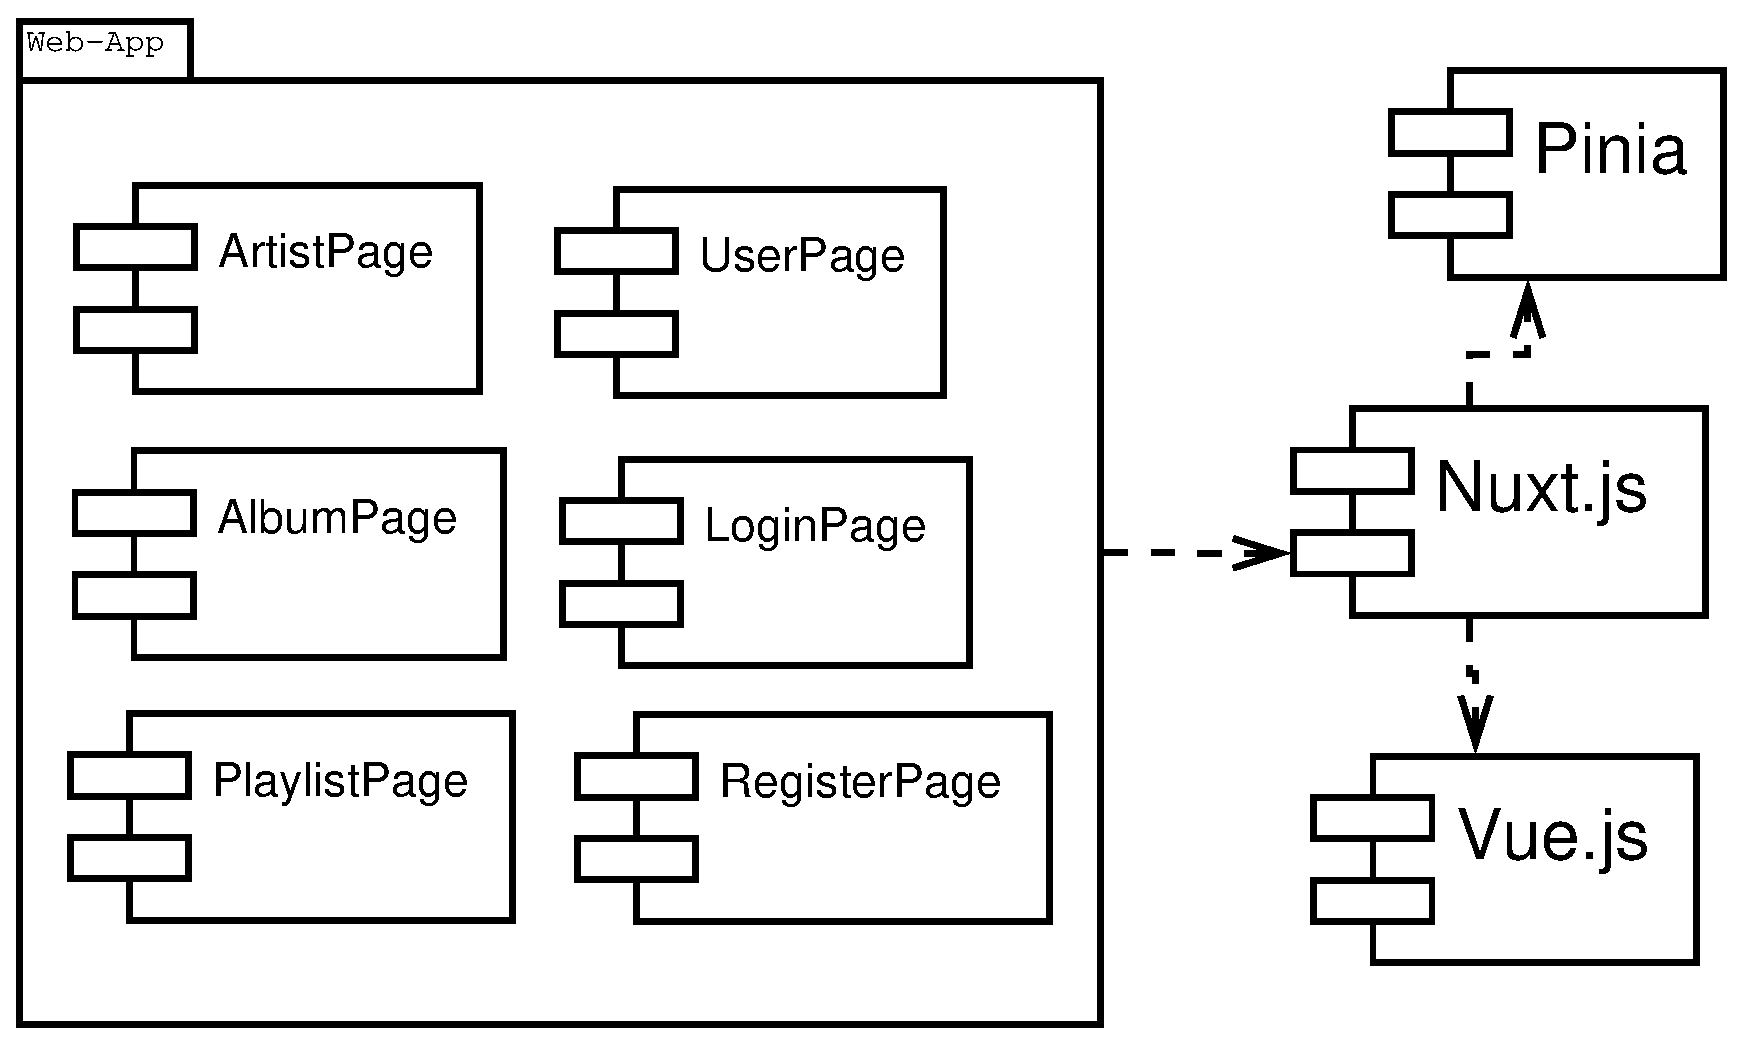
\includegraphics[width=1\linewidth]{frontendComponents}}
\caption{Диаграмма компонентов клиентской части}
\label{frontendComponents:image}
\end{figure}

На рисунке \ref{backendComp:image} изображена диаграмма компонентов для серверной части приложения.

\begin{figure}[ht]
	\center{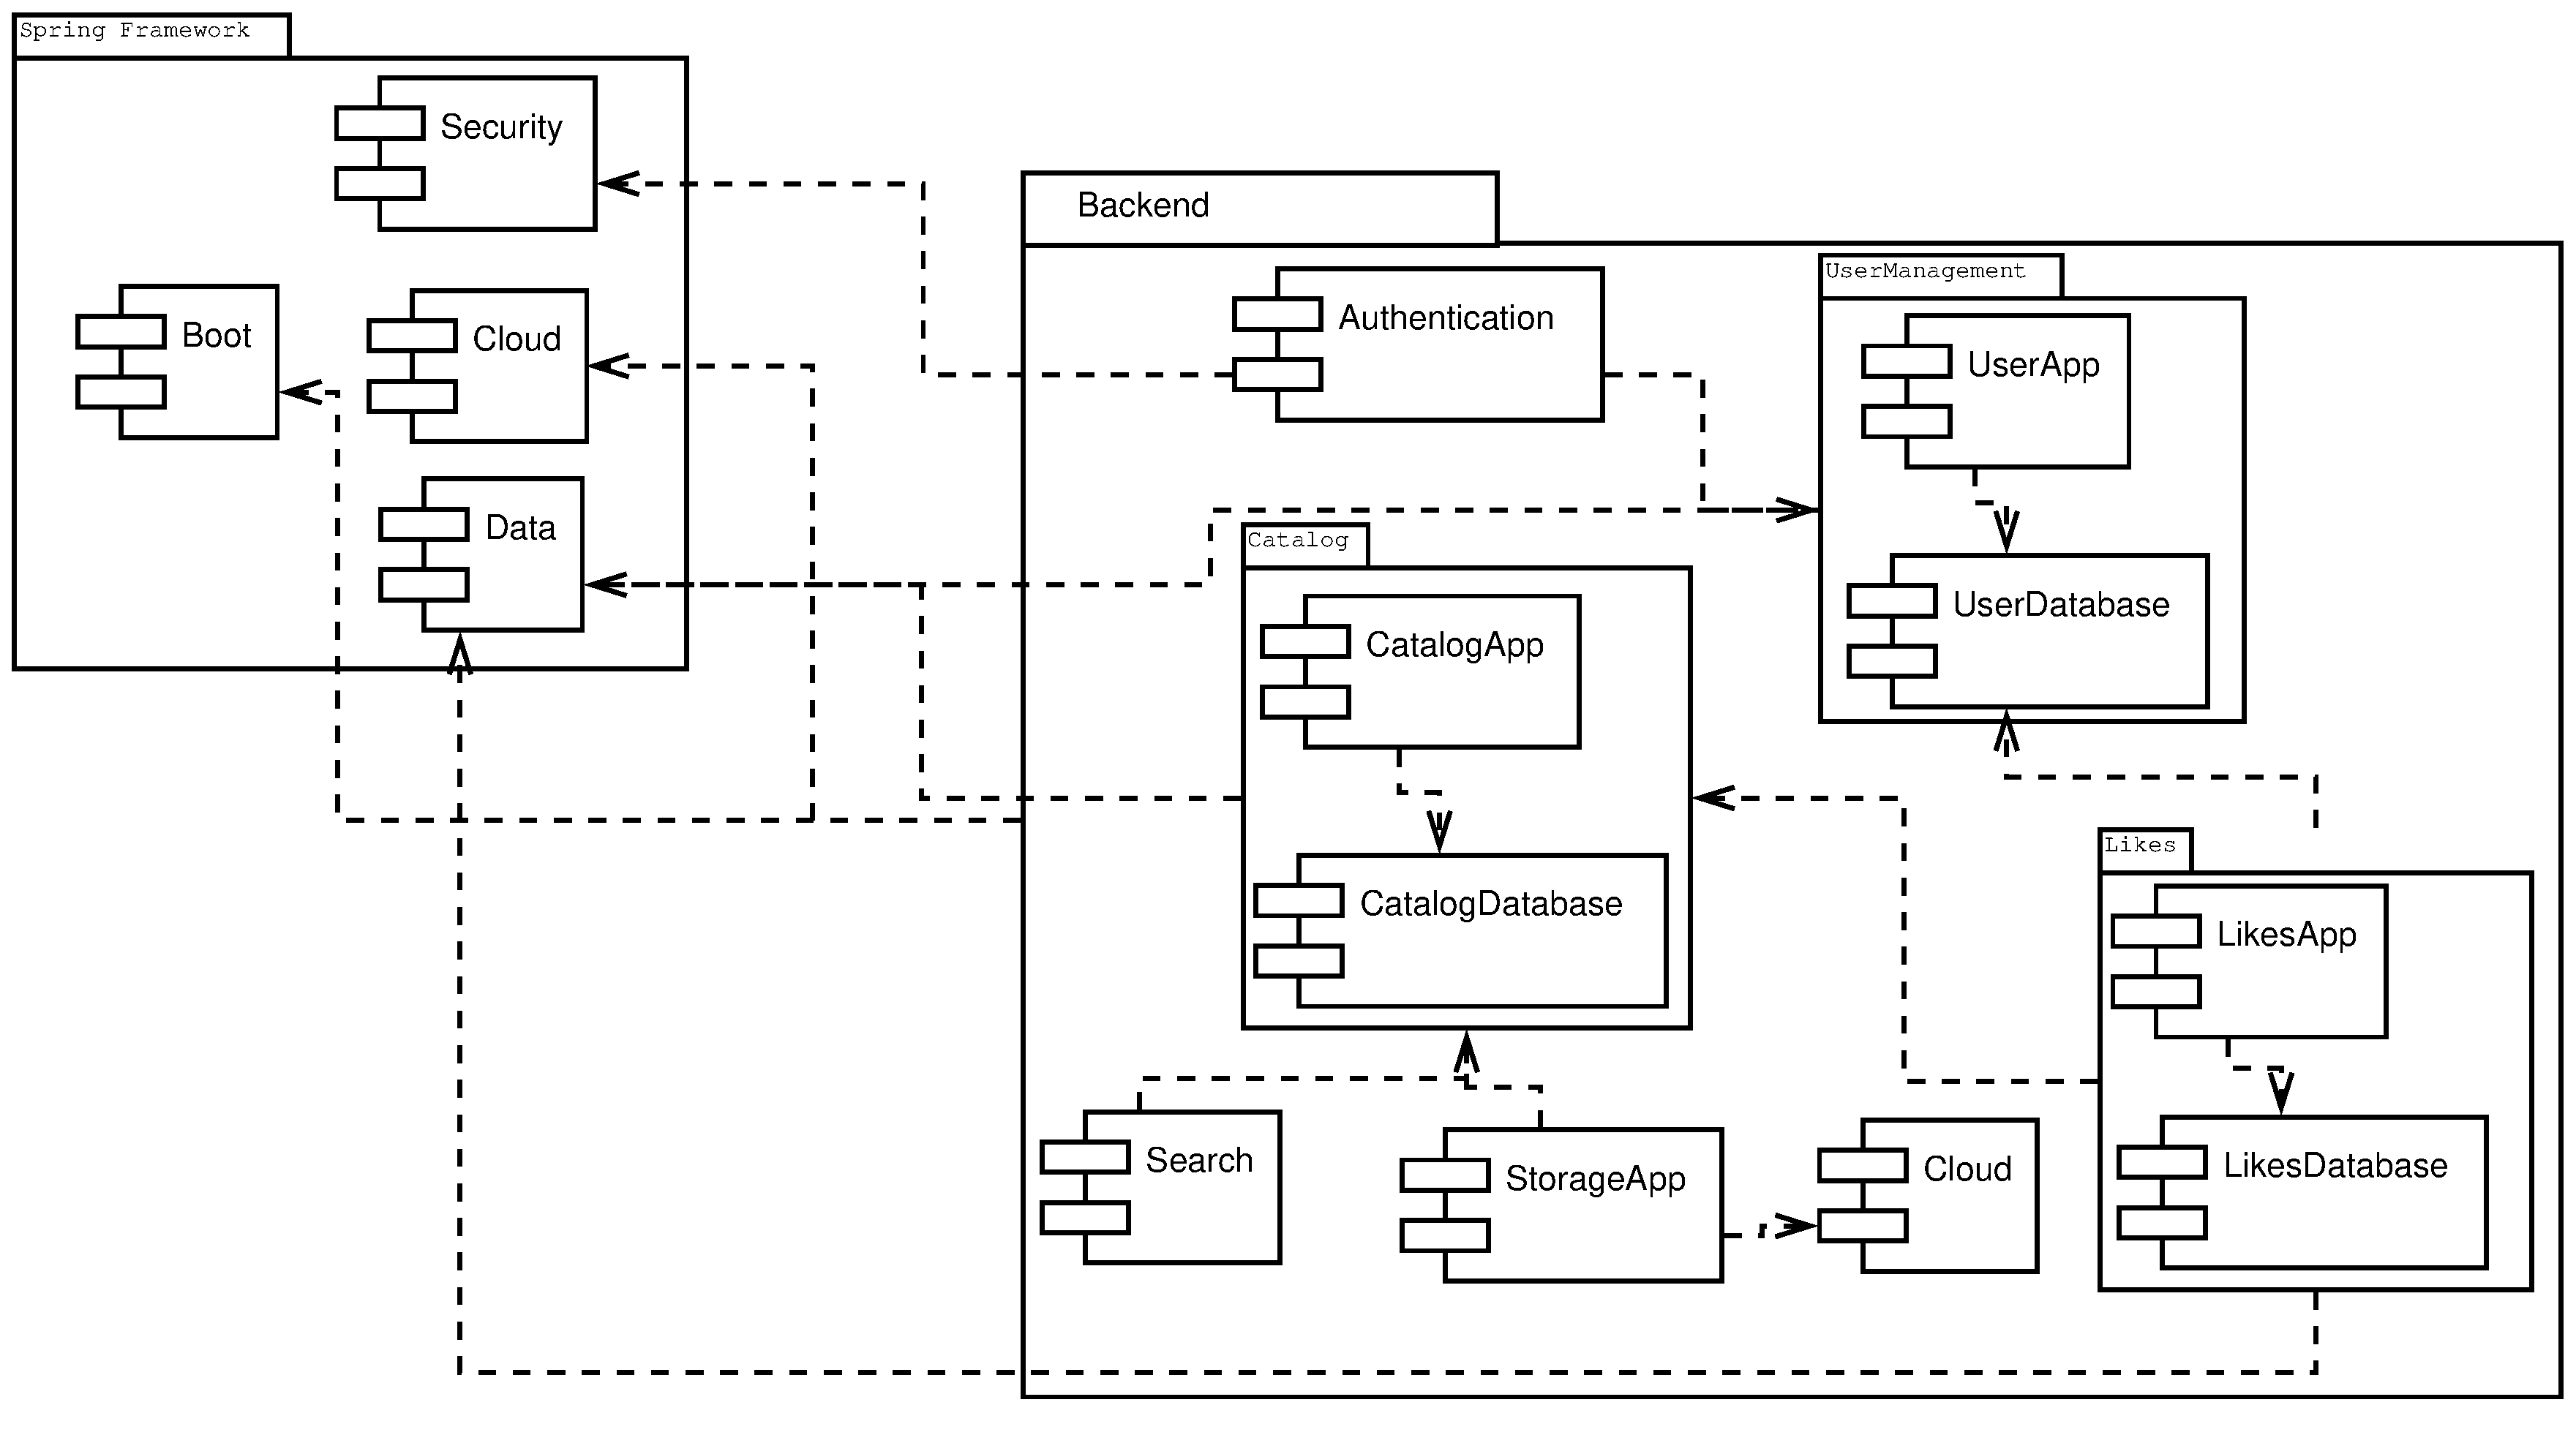
\includegraphics[width=1\linewidth]{backendComp}}
	\caption{Диаграмма компонентов клиентской части}
	\label{backendComp:image}
\end{figure}

Разрабатываемая программная система состоит из клиентской и серверной частей. Клиентская часть представляет собой одностраничное веб-приложение, доступное на любом устройстве, имеющем веб-браузер.
Серверная часть состоит из группы компонентов, отвечающих за разный функционал:
\begin{itemize}
	\item компонент аутентификации выполняет аутентификацию и авторизацию пользователей;
	\item компонент управления пользователями хранит данные пользователей, также отвечает за обработу запросов на изменение данных пользователей;
	\item компонент музыкального каталога отвечет за обрабатку запросов, связанные с музыкальным каталогом;
	\item компонент "<лайков"> хранит "<лайки"> пользователей, обрабатывает запросы на установку и удаление "<лайков">;
	\item компонент поиска обрабатывает поисковые запросы пользователей по музыкальному каталогу;
	\item фйловое хранилище хранит аудиофайлы, обложки альбомов и плейлистов, фото пользоватей.
\end{itemize}

\subsubsection{Компоненты клиентской части}

Клиентская часть представлена приложением на Nuxt3. Страницы Nuxt3 представляют собой Single File Component (однофайловые компоненты) Vue.js, которые совмещают в одном файле шаблон HTML-разметки, стили CSS и логику управления состоянием и данными, написанную на TypeScript.
Разработаны следующие страницы:
\begin{itemize}[]
	\item LoginPage - страница авторизации;
	\item RegisterPage - страница регистрации;
	\item HomePage - страница авторизации;
	\item SearchResultPage - страница авторизации;
	\item ArtistPage - страница исполнителя;
	\item AlbumPage - страница альбома;
	\item PlaylistPage - страница плейлиста;
	\item UserPage - страница пользователя.
\end{itemize}

\subsubsection{Абстракция данных программной системы}
На рисунке \ref{domainClass:image} представлена диаграмма классов предметной области данной системы.

\begin{figure}[ht]
	\center{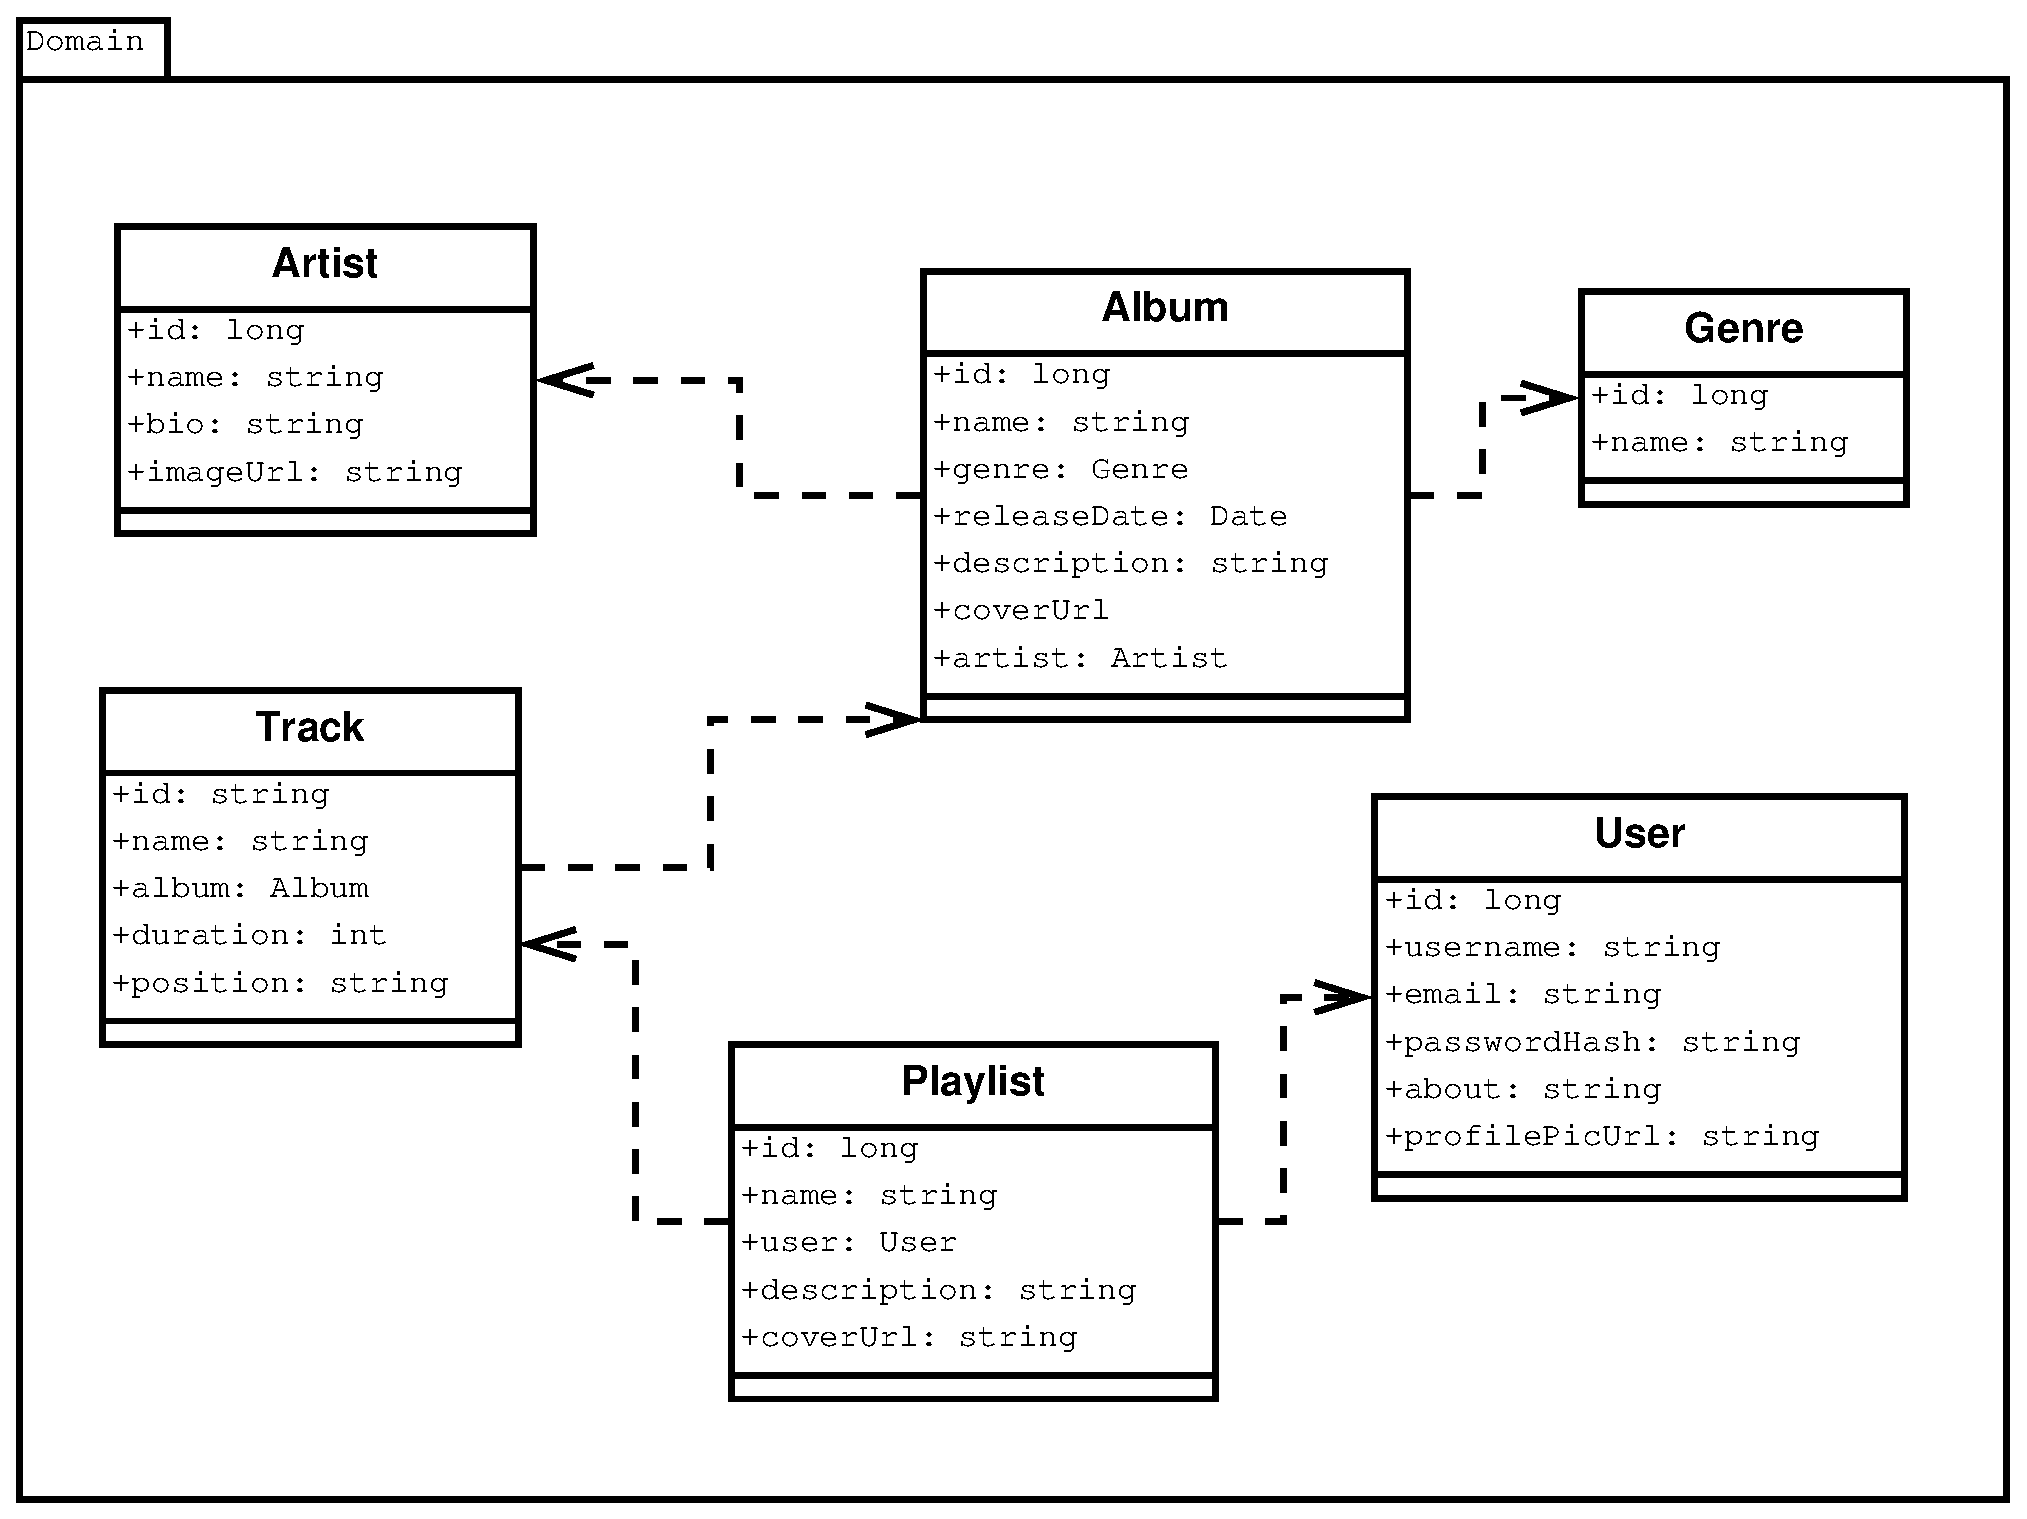
\includegraphics[width=1\linewidth]{domainClass}}
	\caption{Карта маршрутов}
	\label{domainClass:image}
\end{figure}

\subsubsection{Конечные точки серверной части}

Для организации взаимодействия клиентской части с бизнес-логикой приложения были определены конечные точки. На рисунке \ref{routeMap:image} представлена карта маршрутов, представляющая схематическое изображение конечных точек.

\begin{figure}[ht]
	\center{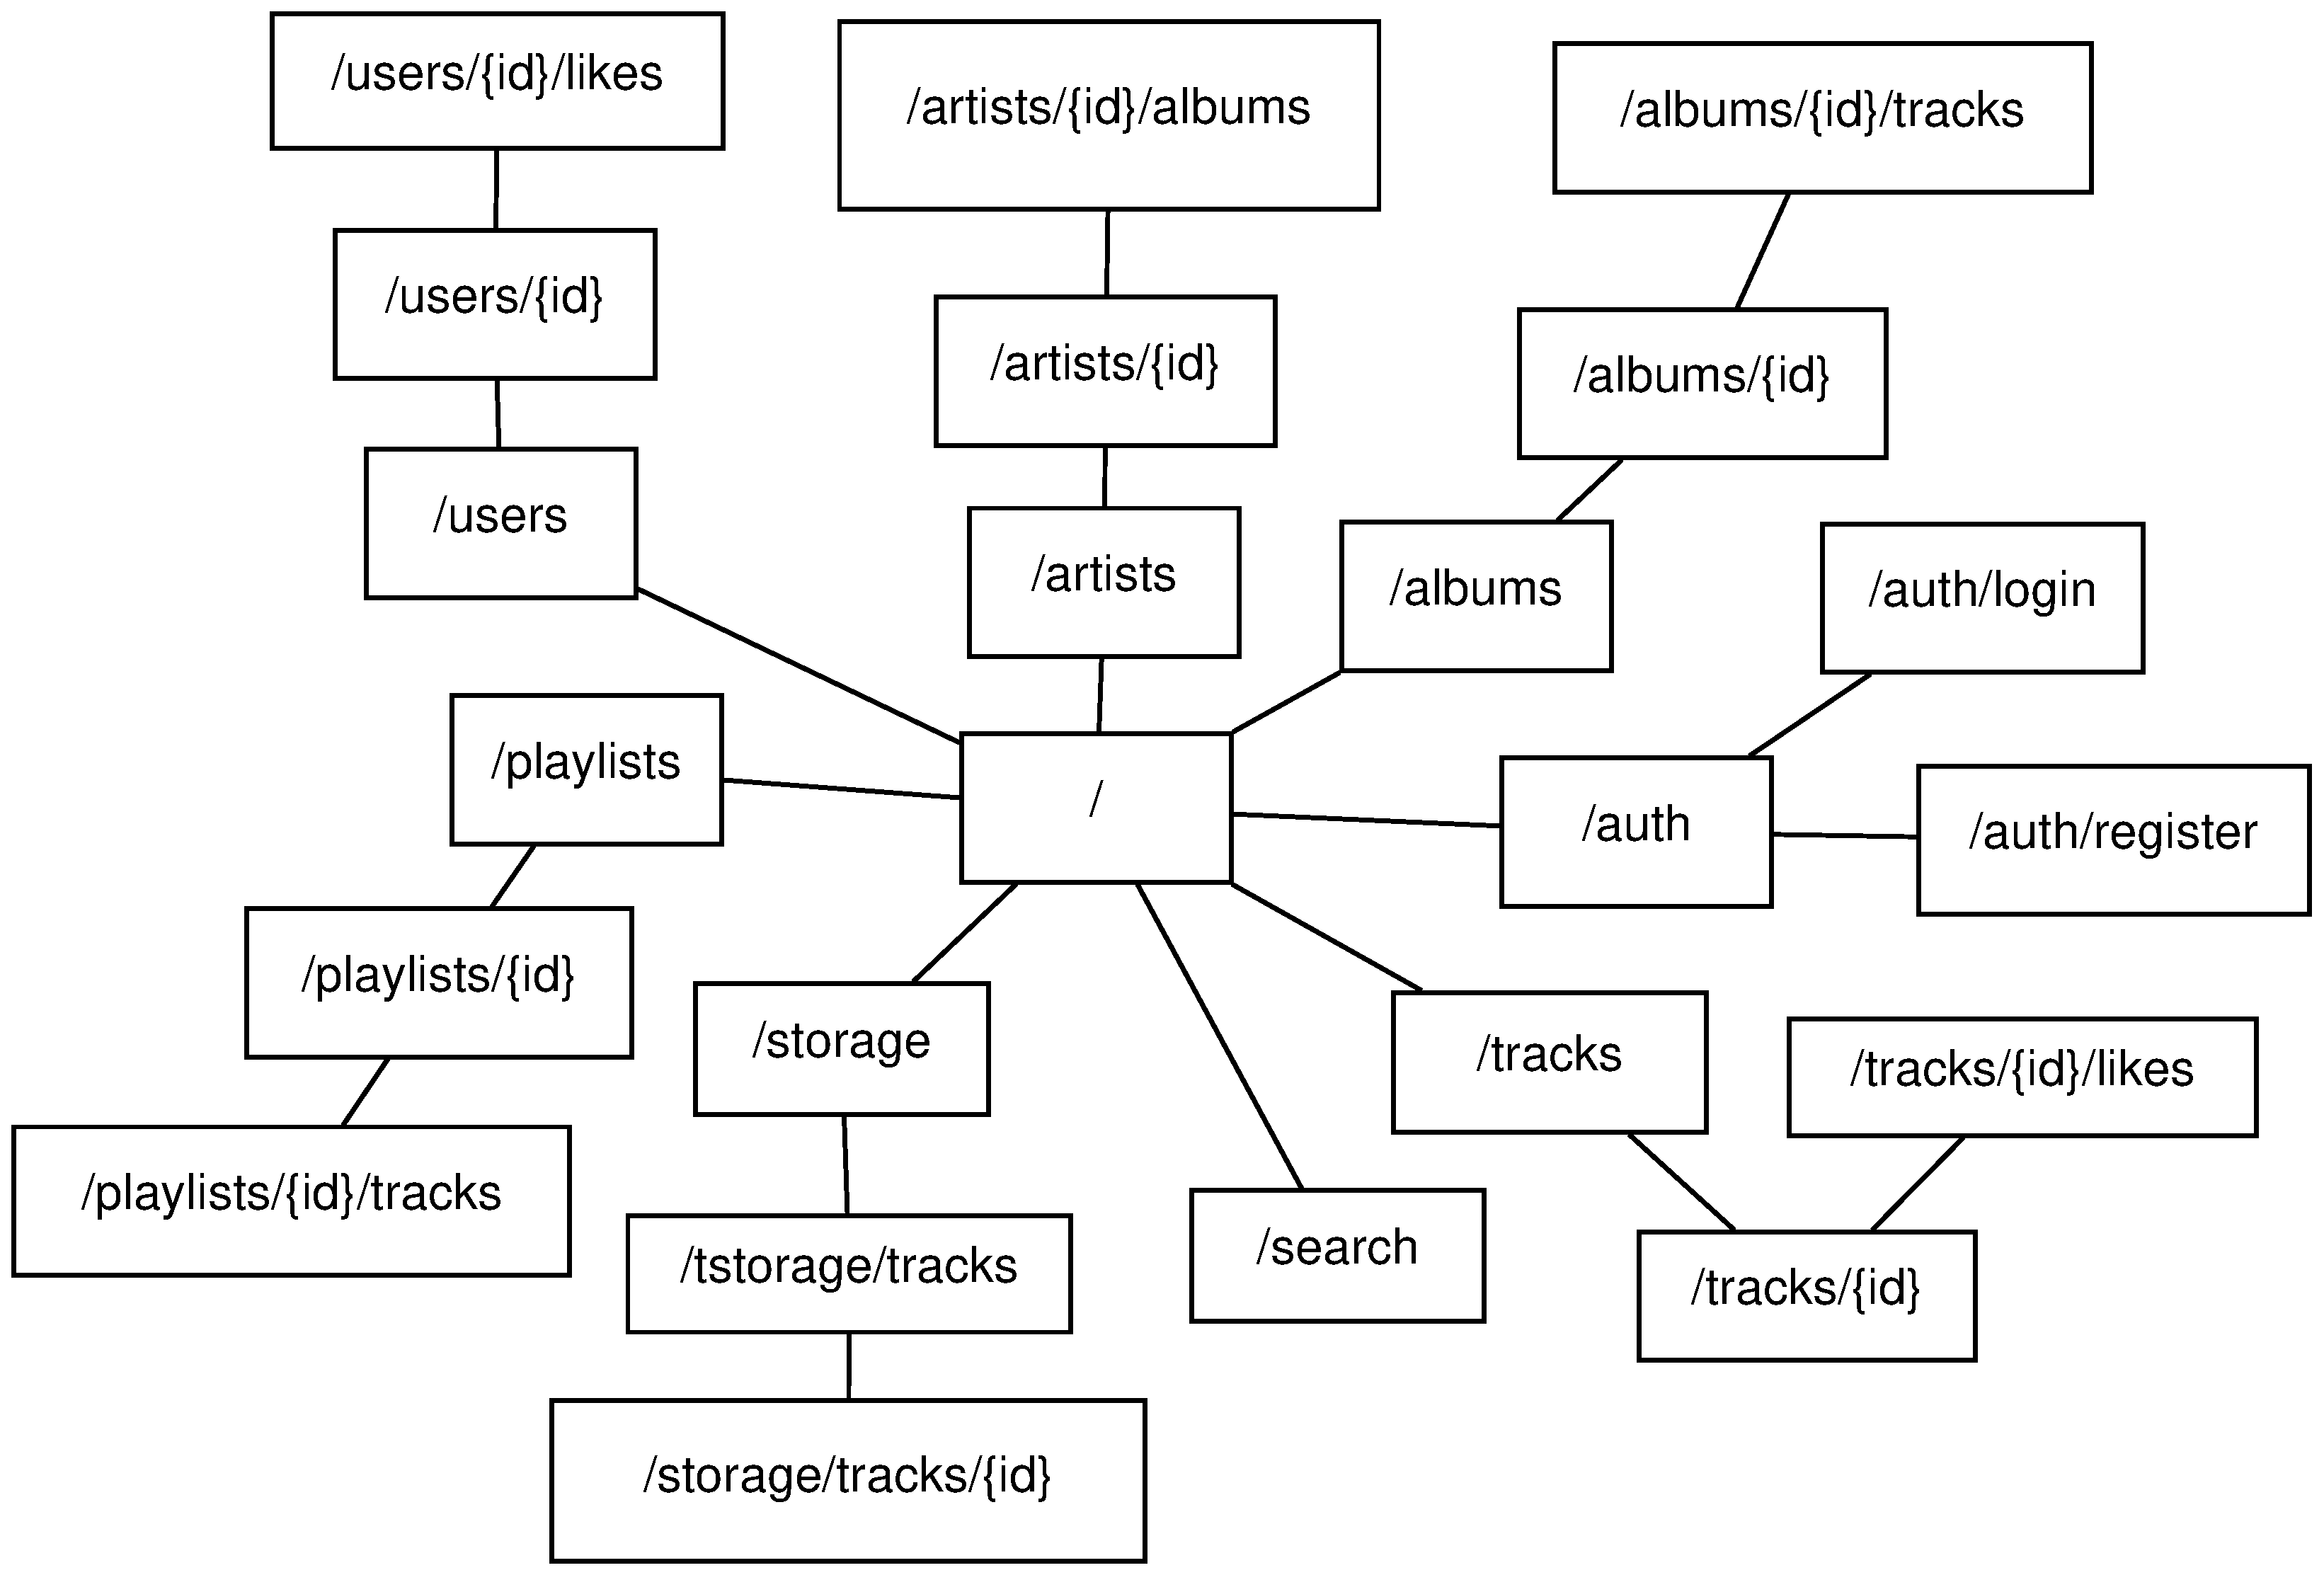
\includegraphics[width=1\linewidth]{routeMap}}
	\caption{Карта маршрутов}
	\label{routeMap:image}
\end{figure}

GET /artists/{id} - предназначен для получения данных об артисте. Принимает параметр id, описывающий идентификатор артиста.

GET /artists/{id}/albums - предназначен для получения списка альбомов артиста. Принимает параметр id, описывающий идентификатор артиста.

GET /albums/{id} - предназначен для получения данных об альбоме. Принимает параметр id, описывающий идентификатор альбома.

GET /albums/{id}/tracks - предназначен для получения списка треков альбома. Принимает параметр id, описывающий идентификатор альбома.

GET /playlists/{id} - предназначен для получения данных о плейлисте. Принимает параметр id, описивающий идентификатор плейлиста.

GET /playlists/{id}/tracks - предназначен для получения списка треков в плейлисте. Принимает параметр id, описивающий идентификатор плейлиста.

POST /playlists - предназначен для создания плейлиста. Принимает в теле запроса JSON-объект, описывающий создаваемый плейлист.

DELETE /playlists/{id} - предназначен для удаления плейлиста. Принимает параметр id, описивающий идентификатор плейлиста.

DELETE /playlists/{id}/tracks - предназначен для удаления треков из плейлиста. Принимает в теле запроса JSON-объект, описывающий список идентификаторов треков, удаляемых из плейлиста и параметр id, описывающий идентификатор плейлиста, из которого удаляются треки. 

PUT /playlists/{id} - предназначен для изменения данных (названия, описания) плейлиста. Принимает в теле запроса JSON-объект, описывающий новые данные о плейлисте. В качестве параметра пути принимает id, описывающий идентификатор плейлиста.

POST /playlists/{id}/tracks - предназначен для добавления треков в плейлист. Принимает в теле запроса JSON-объект, описывающий список идентификаторов треков, добавляемых в плейлист и параметр id, описывающий идентификатор плейлиста, в который добавляются треки. 

POST /auth/login - предназначен для входа пользователя в приожение. Принимает в теле запроса JSON-объект, описывающий данные для аутентификации.

POST /auth/register - предназначен для регистрации пользователя в приложении.  Принимает в теле запроса JSON-объект, описывающий данные для регистрации.

GET /users/{id} - предназначен для получения информации о пользователе. Принимает параметр id, описывающий идентификатор пользователя.

GET /users/likes - предназначен для получения "<лайков"> пользователя.

GET /track/{id}/likes - предназначен для получения "<лайков"> трека. Принимает параметр id, описывающий идентификатор трека, "<лайки"> которого необходимо получить.

POST /track/{id}/likes - предназначен для установки "лайка" трека. Принимает параметр id, описывающий идентификатор трека, "<лайк"> которому необходимо поставить.

POST /track/{id}/likes - предназначен для установки "<лайка"> трека. Принимает параметр id, описывающий идентификатор трека, "<лайк"> которому необходимо поставить.

DELETE /track/{id}/likes - предназначен для удаления "<лайка"> трека. Принимает параметр id, описывающий идентификатор трека, с которого необходимо убрать "<лайк">.

GET /storage/tracks/{id} - предназначен для получения аудиопотока. Принимает параметр id, описывающий идентификатор трека.

GET /search?query={query}\&type={}type - предназначен для поиска в музыкальном каталоге. Принимает строковый параметр query, являющийся строкой запроса, и численный параметр type, обозначающий, в какой категории производится поиск.


\subsection{Проект данных программной системы}

Исходя из требований технического задания, программноинформационная система должна взаимодействовать с двумя типами баз
данных.
SQL\cite{sql1} (реляционные) и NoSQL (нереляционные) являются разными подходами к работе с данными и их хранением. Реляционные базы данных представляют собой базы данных, которые используются для хранения и предоставления доступа к взаимосвязанным элементам информации. Реляционные базы данных основаны на реляционной модели — табличном способе представления данных. Каждая строка, содержащая в таблице такой базы данных, представляет собой запись с уникальным идентификатором, который называют ключом. Столбцы таблицы имеют атрибуты данных, а каждая запись обычно содержит значение для каждого атрибута, что дает возможность легко устанавливать взаимосвязь между элементами данных. Реляционная модель наиболее эффективно поддерживает целостность данных во всех приложениях и копиях (экземплярах) базы данных благодаря соответствию принципам ACID, подразумевающих под собой:
\begin{itemize}
	\item атомарность (англ. atomicity) - никакая транзакция не будет зафиксирована в системе частично;
	\item согласованность (англ. consistency) - каждая успешная транзакция по определению фиксирует только допустимые результаты;
	\item изолированность (англ. isolation) - во время выполнения транзакции параллельные транзакции не должны оказывать влияния на её результат;
	\item устойчивость (англ. durability) - независимо от проблем на нижних уровнях изменения, сделанные успешно завершённой транзакцией, должны остаться сохранёнными после возвращения системы в работу.
\end{itemize}

В отличие от реляционных систем, нереляционные базы данных предлагают гибкость схем данных и способны эффективно масштабироваться для обработки больших объемов данных. NoSQL базы данных часто используют различные структуры данных, такие как ключ-значение, документы, графы и широкие столбцы, что позволяет оптимизировать производительность и удобство разработки в зависимости от характера данных и запросов. Эти системы обычно обеспечивают высокую производительность операций чтения и записи и хорошо подходят для приложений с большими объемами неструктурированных данных. При этом они не обеспечивают такой же устойчивости данных, как реляционный базы.
Основное отличие между SQL и NoSQL заключается в подходах к консистентности данных, масштабируемости и гибкости управления схемами. Реляционные базы данных предпочтительны, когда необходима высокая степень согласованности и точности данных, в то время как нереляционные системы лучше подходят для случаев, когда приоритетны горизонтальное масштабирование и гибкость структуры данных. 

\subsubsection{Описание сущностей серверной части}

В таблице \ref{artist:table} приведены атрибуты и их описание для сущности "<Артист">.

\renewcommand{\arraystretch}{0.8} 
\begin{xltabular}{\textwidth}{|l|l|p{1.7cm}|X|}
	\caption{Атрибуты сущности "<Артист">\label{artist:table}}\\ \hline
	\centrow Поле & \centrow Тип & \centrow Обяза\-тельное & \centrow Описание \\ \hline
	\thead{1} & \thead{2} & \centrow 3 & \centrow 4 \\ \hline
	\endfirsthead
	\continuecaption{Продолжение таблицы \ref{artist:table}}
	\thead{1} & \thead{2} & \centrow 3 & \centrow 4 \\ \hline
	\finishhead
	artist\_id & integer & да & Уникальный идентификатор, автогенерируемый \\ \hline 
	name & character varying(128) & да & Имя артиста \\ \hline 
	bio & character varying(256) & нет & Краткая биорафия \\ \hline 
	image\_url & character varying(256) & нет & Фото артиста \\ \hline 
\end{xltabular}
\renewcommand{\arraystretch}{1.0} 

В таблице \ref{album:table} приведены атрибуты и их описание для сущности "<Альбом">.

\renewcommand{\arraystretch}{0.8} 
\begin{xltabular}{\textwidth}{|l|l|p{1.7cm}|X|}
	\caption{Атрибуты сущности "<Альбом">\label{album:table}}\\ \hline
	\centrow Поле & \centrow Тип & \centrow Обяза\-тельное & \centrow Описание \\ \hline
		\thead{1} & \thead{2} & \centrow 3 & \centrow 4 \\ \hline
	\endfirsthead
	\continuecaption{Продолжение таблицы \ref{album:table}}
	\thead{1} & \thead{2} & \centrow 3 & \centrow 4 \\ \hline
	\finishhead
	album\_id & integer & да & Уникальный идентификатор альбома, автогенерируемый \\ \hline
	artist\_id & integer & да & Идентификатор артиста, внешний ключ \\ \hline
	name & character varying(128) & да & Название альбома \\ \hline
	release\_date & date & да & Дата выпуска \\ \hline
	type & album\_type & да & Тип альбома \\ \hline
	cover\_url & character varying(256) & да & URL обложки альбома \\ \hline
	genre\_id & integer & да & Идентификатор жанра, внешний ключ \\ \hline
\end{xltabular}
\renewcommand{\arraystretch}{1.0}
В таблице \ref{track:table} приведены атрибуты и их описание для сущности "<Трек">.
\renewcommand{\arraystretch}{0.8} 
\begin{xltabular}{\textwidth}{|l|l|p{1.7cm}|X|}
	\caption{Атрибуты сущности "<Трек">\label{track:table}}\\ \hline
	\centrow Поле & \centrow Тип & \centrow Обяза\-тельное & \centrow Описание \\ \hline
		\thead{1} & \thead{2} & \centrow 3 & \centrow 4 \\ \hline
	\endfirsthead
	\continuecaption{Продолжение таблицы \ref{track:table}}
	\thead{1} & \thead{2} & \centrow 3 & \centrow 4 \\ \hline
	\finishhead
	track\_id & integer & да & Уникальный идентификатор трека, автогенерируемый \\ \hline
	album\_id & integer & да & Идентификатор альбома, внешний ключ \\ \hline
	name & character varying(128) & да & Название трека \\ \hline
	duration & integer & да & Длительность трека в секундах \\ \hline
	position & integer & да & Позиция трека в альбоме \\ \hline
\end{xltabular}
\renewcommand{\arraystretch}{1.0}
В таблице \ref{playlist:table} приведены атрибуты и их описание для сущности "<Плейлист">.
\renewcommand{\arraystretch}{0.8} 
\begin{xltabular}{\textwidth}{|l|l|p{1.7cm}|X|}
	\caption{Атрибуты сущности "<Плейлист">\label{playlist:table}}\\ \hline
	\centrow Поле & \centrow Тип & \centrow Обяза\-тельное & \centrow Описание \\ \hline
		\thead{1} & \thead{2} & \centrow 3 & \centrow 4 \\ \hline
	\endfirsthead
	\continuecaption{Продолжение таблицы \ref{playlist:table}}
	\thead{1} & \thead{2} & \centrow 3 & \centrow 4 \\ \hline
	\finishhead
	playlist\_id & integer & да & Уникальный идентификатор плейлиста, автогенерируемый \\ \hline
	user\_login & character varying(128) & да & Логин пользователя, создавшего плейлист \\ \hline
	name & character varying(128) & да & Название плейлиста \\ \hline
	cover\_url & character varying(256) & нет & URL обложки плейлиста \\ \hline
\end{xltabular}
\renewcommand{\arraystretch}{1.0}
В таблице \ref{playlisttrack:table} приведены атрибуты и их описание для сущности "<Связь плейлист-трек">.
\renewcommand{\arraystretch}{0.8} 
\begin{xltabular}{\textwidth}{|l|l|p{1.7cm}|X|}
	\caption{Атрибуты сущности "<Связь плейлист-трек>"\label{playlisttrack:table}}\\ \hline
	\centrow Поле & \centrow Тип & \centrow Обяза\-тельное & \centrow Описание \\ \hline
		\thead{1} & \thead{2} & \centrow 3 & \centrow 4 \\ \hline
	\endfirsthead
	\continuecaption{Продолжение таблицы \ref{playlisttrack:table}}
	\thead{1} & \thead{2} & \centrow 3 & \centrow 4 \\ \hline
	\finishhead
	playlist\_playlist\_id & integer & да & Идентификатор плейлиста, внешний ключ \\ \hline
	track\_track\_id & integer & да & Идентификатор трека, внешний ключ \\ \hline
\end{xltabular}
\renewcommand{\arraystretch}{1.0}
В таблице \ref{genre:table} приведены атрибуты и их описание для сущности "<Жанр">.
\renewcommand{\arraystretch}{0.8} 
\begin{xltabular}{\textwidth}{|l|l|p{1.7cm}|X|}
	\caption{Атрибуты сущности "<Жанр">\label{genre:table}}\\ \hline
	\centrow Поле & \centrow Тип & \centrow Обяза\-тельное & \centrow Описание \\ \hline
		\thead{1} & \thead{2} & \centrow 3 & \centrow 4 \\ \hline
	\endfirsthead
	\continuecaption{Продолжение таблицы \ref{genre:table}}
	\thead{1} & \thead{2} & \centrow 3 & \centrow 4 \\ \hline
	\finishhead
	genre\_id & integer & да & Уникальный идентификатор жанра, автогенерируемый \\ \hline
	name & character varying & да & Название жанра \\ \hline
\end{xltabular}
\renewcommand{\arraystretch}{1.0}
В таблице \ref{user:table} приведены атрибуты и их описание для сущности "<Пользователь">.
\renewcommand{\arraystretch}{0.8} 
\begin{xltabular}{\textwidth}{|l|l|p{1.7cm}|X|}
	\caption{Атрибуты сущности "<Пользователь">\label{user:table}}\\ \hline
	\centrow Поле & \centrow Тип & \centrow Обяза\-тельное & \centrow Описание \\ \hline
		\thead{1} & \thead{2} & \centrow 3 & \centrow 4 \\ \hline
	\endfirsthead
	\continuecaption{Продолжение таблицы \ref{user:table}}
	\thead{1} & \thead{2} & \centrow 3 & \centrow 4 \\ \hline
	\finishhead
	user\_id & integer & да & Уникальный идентификатор пользователя, автогенерируемый \\ \hline 
	username & character varying(128) & да & Имя пользователя, уникальное в системе \\ \hline 
	email & character varying(256) & да & Электронная почта пользователя, уникальная в системе \\ \hline 
	password\_hash & character varying(256) & да & Хеш пароля для безопасности аутентификации \\ \hline 
	password\_salt & character varying(256) & да & Соль для хеширования пароля, уникальная для каждого пользователя \\ \hline 
	bio & text & нет & Краткая биография пользователя, необязательное поле \\ \hline 
	photo & character varying(256) & нет & URL фотографии профиля пользователя \\ \hline 
\end{xltabular}
\renewcommand{\arraystretch}{1.0}
В таблице \ref{like:table} приведены атрибуты и их описание для сущности "<Лайк">.
\renewcommand{\arraystretch}{0.8} 
\begin{xltabular}{\textwidth}{|l|l|p{1.7cm}|X|}
	\caption{Атрибуты сущности "<Лайк">\label{like:table}}\\ \hline
	\centrow Поле & \centrow Тип & \centrow Обяза\-тельное & \centrow Описание \\ \hline
		\thead{1} & \thead{2} & \centrow 3 & \centrow 4 \\ \hline
	\endfirsthead
	\continuecaption{Продолжение таблицы \ref{like:table}}
	\thead{1} & \thead{2} & \centrow 3 & \centrow 4 \\ \hline
	\finishhead
	\_id & ObjectId & да & Уникальный идентификатор лайка, автогенерируемый \\ \hline 
	user\_id & Long & да & Идентификатор пользователя, который поставил лайк \\ \hline 
	track\_id & Long & да & Идентификатор трека, которому поставлен лайк \\ \hline 
\end{xltabular}
\renewcommand{\arraystretch}{1.0}
\subsection{Проектирование пользовательского интерфейса}

После анализа требований к интерфейсу пользователя\cite{ui}, описанных в разделе технического задания, был разработан графический интерфейс для взаимодействия с приложением. Интерфейс разработан с применением javaScript- фреймворка Nuxt.js, основанного на Vue.js. Для стилизации элементов был использован CSS 3.
На представленных ниже рисунках числами обозначены элементы графического интерфейса.
На рисунке \ref{regMaket:image} представлен макет страницы регистрации. Элементы страницы регистрации:
\begin{enumerate}
	\item Форма регистрации.
	\item Поле ввода имени пользователя.
	\item Поле ввода электронной почты.
	\item Поле ввода пароля.
	\item Поле подтверждения пароля.
	\item Кнопка подтверждения формы.
\end{enumerate} 

\begin{figure}[ht]
	\center{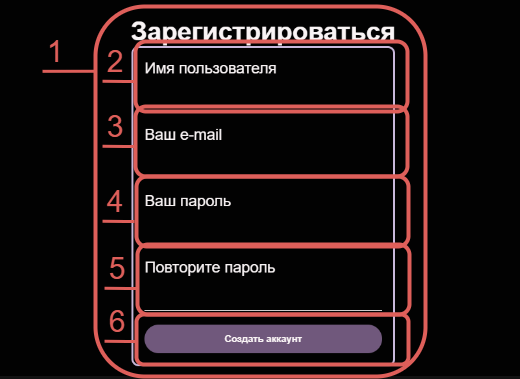
\includegraphics[width=1\linewidth]{regMaket}}
	\caption{Макет страницы регистрации}
	\label{regMaket:image}
\end{figure}
На рисунке \ref{loginMaket:image} представлен макет страницы входа. Элементы страницы входа:
\begin{enumerate}
	\item Форма входа.
	\item Поле ввода электронной почты.
	\item Поле ввода пароля.
	\item Кнопка подтверждения формы.
	\item Ссылка на страницу регистрации.
\end{enumerate} 
\begin{figure}[H]
	\center{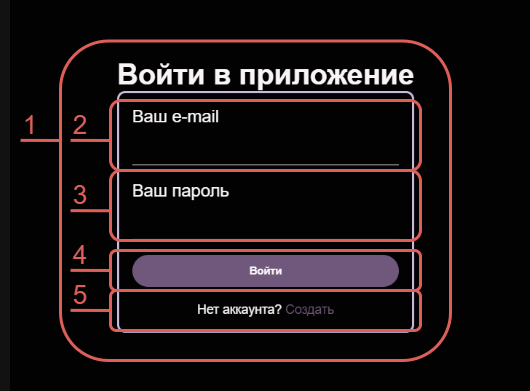
\includegraphics[width=0.8\linewidth]{loginMaket}}
	\caption{Макет страницы входа}
	\label{loginMaket:image}
\end{figure}
На рисунке \ref{artistMaket:image} представлен макет страницы исполнителя. Элементы страницы исполнителя:
	\begin{enumerate}
		\item Фото исполнителя.
		\item Информация о исполнителе.
		\item Список альбомов исполнителя.
		\item Карточка с информацией об альбоме.
		\item Ссылка на страницу альбома.
	\end{enumerate} 
\begin{figure}[H]
	\center{
\includegraphics[width=0.8\linewidth]{artistMaket}}
	\caption{Макет страницы исполнителя}
	\label{artistMaket:image}
\end{figure}
На рисунке \ref{albumMaket:image} представлен макет страницы альбома. Элементы страницы альбома:
\begin{enumerate}
	\item Обложка альбома.
	\item Информация об альбоме.
	\item Список треков.
	\item Строка трека.
	\item Информация о треке.
	\item Кнопка запуска проигрывания.
\end{enumerate} 
\begin{figure}[ht]
	\center{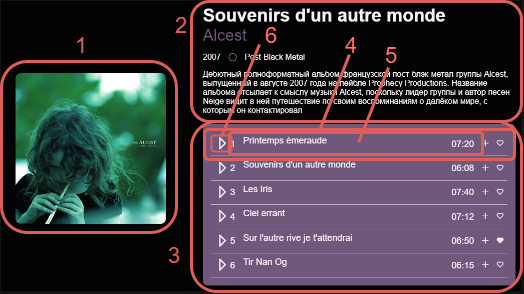
\includegraphics[width=0.85\linewidth]{albumMaket}}
	\caption{Макет страницы альбома}
	\label{albumMaket:image}
\end{figure}


\ifПрактика{}\else{
   \section{Рабочий проект}
\subsection{Спецификация разработанных класов и компонентов}

В результате разработки программного продукта были реализованы классы и компоненты, обеспечивающие работоспособность системы. Спецификация классов и компонентов описана в данной главе.

\subsubsection{Спецификация класса ArtistController}
Данный класс является контроллером, обрабатывающим запросы,связанные с артистами. Описание класса представлено в таблице \ref{classArtist:table}

\renewcommand{\arraystretch}{0.8} % уменьшение расстояний до сетки таблицы
\begin{xltabular}{\textwidth}{|X|p{2.5cm}|>{\setlength{\baselineskip}{0.7\baselineskip}}p{4.85cm}|>{\setlength{\baselineskip}{0.7\baselineskip}}p{4.85cm}|}
	\caption{Описание класса ArtistController\label{classArtist:table}}\\
	\hline \centrow \setlength{\baselineskip}{0.7\baselineskip} Название поля(метода) & \centrow \setlength{\baselineskip}{0.7\baselineskip} Область видимости & \centrow Тип значения & \centrow Описание \\
	\hline \centrow 1 & \centrow 2 & \centrow 3 & \centrow 4\\ \hline
	\endfirsthead
	\continuecaption{Продолжение таблицы\ref{classArtist:table}}
	\hline \centrow 1 & \centrow 2 & \centrow 3 & \centrow 4\\ \hline
	\finishhead
	artistService & private & ArtistService & Объект, отвечающий за бизнес-логику сущности "<Artist"> \\
	\hline albumService & private & AlbumService & Объект, отвечающий за бизнес-логику сущности "<Album"> \\
	\hline getArtist ById & public & ResponseEntity <ArtistDto> & Возвращает артиста по идентификатору. Входные параметры: id - идентификатор артиста \\
	\hline getArtist Albums & public & ResponseEntity <ArtistDto> & Возвращает артиста со списком альбомов по идентификатору. Входные параметры: id - идентификатор артиста 
\end{xltabular}
\renewcommand{\arraystretch}{1.0} % восстановление сетки


\subsubsection{Спецификация класса AlbumController}
Данный класс является контроллером, обрабатывающим запросы, связанные с альбомами. Описание класса представлено в таблице \ref{classAlbum:table}

\begin{xltabular}{\textwidth}{|X|p{2.5cm}|>{\setlength{\baselineskip}{0.7\baselineskip}}p{4.85cm}|>{\setlength{\baselineskip}{0.7\baselineskip}}p{4.85cm}|}
	\caption{Описание класса AlbumController}\label{classAlbum:table}\\
	\hline \centrow \setlength{\baselineskip}{0.7\baselineskip} Название поля(метода) & \centrow \setlength{\baselineskip}{0.7\baselineskip} Область видимости & \centrow Тип значения & \centrow Описание \\
	\hline \centrow 1 & \centrow 2 & \centrow 3 & \centrow 4\\ \hline
	\endfirsthead
	\continuecaption{Продолжение таблицы \ref{classAlbum:table}}
	\hline \centrow 1 & \centrow 2 & \centrow 3 & \centrow 4\\ \hline
	\finishhead
	albumService & private & AlbumService & Объект, отвечающий за бизнес-логику сущности "<Album"> \\
	\hline trackService & private & TrackService & Объект, отвечающий за бизнес-логику сущности "<Track"> \\
	\hline getAlbum ById & public & ResponseEntity <AlbumDto> & Возвращает альбом по идентификатору. Входные параметры: id - идентификатор альбома 
\end{xltabular}

\subsubsection{Спецификация класса PlaylistController}
Данный класс является контроллером, обрабатывающим запросы, связанные с плейлистами. Описание класса представлено в таблице \ref{classPlaylist:table}.

\begin{xltabular}{\textwidth}{|X|p{2.5cm}|>{\setlength{\baselineskip}{0.7\baselineskip}}p{4.83cm}|>{\setlength{\baselineskip}{0.7\baselineskip}}p{4.85cm}|}
	\caption{Описание класса PlaylistController}\label{classPlaylist:table}\\
	\hline \centrow \setlength{\baselineskip}{0.7\baselineskip} Название поля(метода) & \centrow \setlength{\baselineskip}{0.7\baselineskip} Область видимости & \centrow Тип значения & \centrow Описание \\
	\hline \centrow 1 & \centrow 2 & \centrow 3 & \centrow 4\\ \hline
	\endfirsthead
	\continuecaption{Продолжение таблицы \ref{classPlaylist:table}}
	\hline \centrow 1 & \centrow 2 & \centrow 3 & \centrow 4\\ \hline
	\finishhead
	playlist Service & private & PlaylistService & Объект, отвечающий за бизнес-логику сущности "<Playlist"> \\
	\hline getPlaylist Info & public & ResponseEntity <PlaylistDetailsDto> & Возвращает информацию о плейлисте по идентификатору. Входные параметры: id - идентификатор плейлиста \\
	\hline getPlaylist Tracklist & public & ResponseEntity <PlaylistTracklistDto> & Возвращает список треков плейлиста по идентификатору. Входные параметры: id - идентификатор плейлиста \\
	\hline createNew Playlist & public & ResponseEntity <PlaylistCreatedDto> & Создает новый плейлист. Входные параметры: newPlaylist - объект, содержащий данные нового плейлиста \\
	\hline deletePlaylist & public & ResponseEntity <?> & Удаляет плейлист по идентификатору. Входные параметры: id - идентификатор плейлиста \\
	\hline addTracksTo Playlist & public & ResponseEntity <?> & Добавляет треки в плейлист по идентификатору. Входные параметры: id - идентификатор плейлиста, tracks - объект, содержащий список идентификаторов треков \\
	\hline removeTracks FromPlaylist & public & ResponseEntity <PlaylistTracklistDto> & Удаляет треки из плейлиста по идентификатору. Входные параметры: id - идентификатор плейлиста, tracks - объект, содержащий список идентификаторов треков \\
	\hline updatePlaylist Details & public & ResponseEntity <PlaylistDetailsDto> & Обновляет детали плейлиста по идентификатору. Входные параметры: id - идентификатор плейлиста, newDetails - объект, содержащий новые данные плейлиста 
\end{xltabular}

\subsubsection{Спецификация класса TrackController}
Данный класс является контроллером, обрабатывающим запросы, связанные с плейлистами. Описание класса представлено в таблице \ref{classTrack:table}.

\renewcommand{\arraystretch}{0.8} % уменьшение расстояний до сетки таблицы
\begin{xltabular}{\textwidth}{|X|p{2.5cm}|>{\setlength{\baselineskip}{0.7\baselineskip}}p{4.83cm}|>{\setlength{\baselineskip}{0.7\baselineskip}}p{4.85cm}|}
	\caption{Описание класса TrackController}\label{classTrack:table}\\
	\hline \centrow \setlength{\baselineskip}{0.7\baselineskip} Название поля(метода) & \centrow \setlength{\baselineskip}{0.7\baselineskip} Область видимости & \centrow Тип значения & \centrow Описание \\
	\hline \centrow 1 & \centrow 2 & \centrow 3 & \centrow 4\\ \hline
	\endfirsthead
	\continuecaption{Продолжение таблицы \ref{classTrack:table}}
	\hline \centrow 1 & \centrow 2 & \centrow 3 & \centrow 4\\ \hline
	\finishhead
	trackService & private & TrackService & Объект, отвечающий за бизнес-логику сущности "<Track"> \\
	\hline isTrackExists & public & ResponseEntity <BooleanResponse> & Проверяет существование трека по идентификатору. Входные параметры: id - идентификатор трека \\
\end{xltabular}
\renewcommand{\arraystretch}{1.0}

\subsubsection{Спецификация класса UserManagementController}
Данный класс является контроллером, обрабатывающим запросы, связанные с пользователем. Описание класса представлено в таблице \ref{classUsers:table}.

\renewcommand{\arraystretch}{0.8} % уменьшение расстояний до сетки таблицы
\begin{xltabular}{\textwidth}{|X|p{2.5cm}|>{\setlength{\baselineskip}{0.7\baselineskip}}p{4.83cm}|>{\setlength{\baselineskip}{0.7\baselineskip}}p{4.85cm}|}
	\caption{Описание класса UserManagementController}\label{classUsers:table}\\
	\hline \centrow \setlength{\baselineskip}{0.7\baselineskip} Название поля(метода) & \centrow \setlength{\baselineskip}{0.7\baselineskip} Область видимости & \centrow Тип значения & \centrow Описание \\
	\hline \centrow 1 & \centrow 2 & \centrow 3 & \centrow 4\\ \hline
	\endfirsthead
	\continuecaption{Продолжение таблицы \ref{classUsers:table}}
	\hline \centrow 1 & \centrow 2 & \centrow 3 & \centrow 4\\ \hline
	\finishhead
	userManage mentService & private & UserManagement Service & Объект, отвечающий за бизнес-логику управления пользователями \\
	\hline getUserBy Username & public & ResponseEntity <User> & Возвращает пользователя по имени пользователя. Входные параметры: username - имя пользователя \\
	\hline getUserBy Email & public & ResponseEntity <User> & Возвращает пользователя по адресу электронной почты. Входные параметры: email - адрес электронной почты пользователя \\
	\hline getUserById & public & ResponseEntity <PublicUserDto> & Возвращает пользователя по идентификатору. Входные параметры: id - идентификатор пользователя \\
	\hline createUser & public & ResponseEntity <?> & Создает нового пользователя. Входные параметры: user - объект, содержащий данные нового пользователя \\
	\hline deleteUser & public & ResponseEntity <?> & Удаляет пользователя по идентификатору. Входные параметры: id - идентификатор пользователя 
\end{xltabular}
\renewcommand{\arraystretch}{1.0}

\subsubsection{Спецификация класса TrackStorageContoller}
Данный класс является сервисом, обрабатывающим бизнес-логику, связанную с управлением пользователями. Описание класса представлено в таблице \ref{classStorage:table}.

\renewcommand{\arraystretch}{0.8} % уменьшение расстояний до сетки таблицы
\begin{xltabular}{\textwidth}{|X|p{2.5cm}|>{\setlength{\baselineskip}{0.7\baselineskip}}p{4.83cm}|>{\setlength{\baselineskip}{0.7\baselineskip}}p{4.85cm}|}
	\caption{Описание класса TrackController}\label{classStorage:table}\\
	\hline \centrow \setlength{\baselineskip}{0.7\baselineskip} Название поля(метода) & \centrow \setlength{\baselineskip}{0.7\baselineskip} Область видимости & \centrow Тип значения & \centrow Описание \\
	\hline \centrow 1 & \centrow 2 & \centrow 3 & \centrow 4\\ \hline
	\endfirsthead
	\continuecaption{Продолжение таблицы \ref{classStorage:table}}
	\hline \centrow 1 & \centrow 2 & \centrow 3 & \centrow 4\\ \hline
	\finishhead
	audioStream Loader & private & AudioStream Loader & Объект, отвечающий за организацию потока аудио \\
	\hline getTrack & public & ResponseEntity <StreamingResponseBody> & Метод, отвечающий за передачу частей аудио. Входные параметры: id - идентификатор трека\\
\end{xltabular}
\renewcommand{\arraystretch}{1.0}

\subsubsection{Спецификация класса ArtistService}
Данный класс обеспечивает бизнес-логику, связанную с исполнителями. Описание класса представлено в таблице \ref{classArtistService:table}.

\renewcommand{\arraystretch}{0.8} % уменьшение расстояний до сетки таблицы
\begin{xltabular}{\textwidth}{|X|p{2.5cm}|>{\setlength{\baselineskip}{0.7\baselineskip}}p{4.83cm}|>{\setlength{\baselineskip}{0.7\baselineskip}}p{4.85cm}|}
	\caption{Описание класса ArtistService}\label{classArtistService:table}\\
	\hline \centrow \setlength{\baselineskip}{0.7\baselineskip} Название поля(метода) & \centrow \setlength{\baselineskip}{0.7\baselineskip} Область видимости & \centrow Тип значения & \centrow Описание \\
	\hline \centrow 1 & \centrow 2 & \centrow 3 & \centrow 4\\ \hline
	\endfirsthead
	\continuecaption{Продолжение таблицы \ref{classArtistService:table}}
	\hline \centrow 1 & \centrow 2 & \centrow 3 & \centrow 4\\ \hline
	\finishhead
	artistsRepo sitory & private & ArtistsRepository & Репозиторий, отвечающий за доступ к данным артистов \\
	\hline getArtist ById & public & Optional <ArtistDto> & Возвращает артиста по идентификатору. Входные параметры: id - идентификатор артиста \\
	\hline getArtist WithAlbums & public & Optional <ArtistDto> & Возвращает артиста с альбомами по идентификатору. Входные параметры: id - идентификатор артиста 
\end{xltabular}
\renewcommand{\arraystretch}{1.0}

\subsubsection{Спецификация класса AlbumService}
Данный класс является сервисом, обрабатывающим бизнес-логику, связанную с альбомами. Описание класса представлено в таблице \ref{classAlbumService:table}.

\renewcommand{\arraystretch}{0.8} % уменьшение расстояний до сетки таблицы
\begin{xltabular}{\textwidth}{|X|p{2.5cm}|>{\setlength{\baselineskip}{0.7\baselineskip}}p{4.83cm}|>{\setlength{\baselineskip}{0.7\baselineskip}}p{4.85cm}|}
	\caption{Описание класса AlbumService}\label{classAlbumService:table}\\
	\hline \centrow \setlength{\baselineskip}{0.7\baselineskip} Название поля(метода) & \centrow \setlength{\baselineskip}{0.7\baselineskip} Область видимости & \centrow Тип значения & \centrow Описание \\
	\hline \centrow 1 & \centrow 2 & \centrow 3 & \centrow 4\\ \hline
	\endfirsthead
	\continuecaption{Продолжение таблицы \ref{classAlbumService:table}}
	\hline \centrow 1 & \centrow 2 & \centrow 3 & \centrow 4\\ \hline
	\finishhead
	albumRepo sitory & private & AlbumRepository & Репозиторий, отвечающий за доступ к данным альбомов \\
	\hline findAlbum ById & public & Optional <Album> & Возвращает альбом по идентификатору. Входные параметры: id - идентификатор альбома \\
	\hline findArtist Albums & public & List <AlbumOfArtistPreviewDto> & Возвращает список альбомов по идентификатору артиста. Входные параметры: artistId - идентификатор артиста 
\end{xltabular}
\renewcommand{\arraystretch}{1.0}


\subsubsection{Спецификация класса PlaylistService}
Данный класс является сервисом, обрабатывающим бизнес-логику, связанную с плейлистами. Описание класса представлено в таблице \ref{classPlaylistService:table}.

\renewcommand{\arraystretch}{0.8} % уменьшение расстояний до сетки таблицы
\begin{xltabular}{\textwidth}{|X|p{2.5cm}|>{\setlength{\baselineskip}{0.7\baselineskip}}p{4.83cm}|>{\setlength{\baselineskip}{0.7\baselineskip}}p{4.85cm}|}
	\caption{Описание класса PlaylistService}\label{classPlaylistService:table}\\
	\hline \centrow \setlength{\baselineskip}{0.7\baselineskip} Название поля(метода) & \centrow \setlength{\baselineskip}{0.7\baselineskip} Область видимости & \centrow Тип значения & \centrow Описание \\
	\hline \centrow 1 & \centrow 2 & \centrow 3 & \centrow 4\\ \hline
	\endfirsthead
	\continuecaption{Продолжение таблицы \ref{classPlaylistService:table}}
	\hline \centrow 1 & \centrow 2 & \centrow 3 & \centrow 4\\ \hline
	\finishhead
	playlistRepo sitory & private & PlaylistRepository & Репозиторий, отвечающий за доступ к данным плейлистов \\
	\hline trackService & private & TrackService & Объект, отвечающий за бизнес-логику сущности "<Track"> \\
	\hline userManagement Client & private & UserManage mentClient & Объект, отвечающий за взаимодействие с сервисом управления пользователями \\
	\hline getTracksBy PlaylistId & public & Set <Track> & Возвращает треки плейлиста по идентификатору. Входные параметры: playlistId - идентификатор плейлиста \\
	\hline getPlaylist ById & public & Optional <Playlist> & Возвращает плейлист по идентификатору. Входные параметры: playlistId - идентификатор плейлиста \\
	\hline createNew Playlist & public & Long & Создает новый плейлист. Входные параметры: newPlaylist - объект, содержащий данные нового плейлиста \\
	\hline removePlay listById & public & void & Удаляет плейлист по идентификатору. Входные параметры: id - идентификатор плейлиста \\
	\hline getPlaylist DtoById & public & Optional <PlaylistDto> & Возвращает DTO плейлиста по идентификатору. Входные параметры: id - идентификатор плейлиста \\
	\hline addTracks ToPlaylist & public & PlaylistTrack listDto & Добавляет треки в плейлист. Входные параметры: id - идентификатор плейлиста, trackIds - идентификаторы треков \\
	\hline removeTracks FromPlaylist & public & PlaylistTrack listDto & Удаляет треки из плейлиста. Входные параметры: id - идентификатор плейлиста, trackIds - идентификаторы треков \\
	\hline getPlaylist InfoById & public & PlaylistDetailsDto & Возвращает информацию о плейлисте по идентификатору. Входные параметры: id - идентификатор плейлиста \\
	\hline getPlaylist Tracklist & public & PlaylistTrack listDto & Возвращает треклист плейлиста по идентификатору. Входные параметры: playlistId - идентификатор плейлиста 
\end{xltabular}
\renewcommand{\arraystretch}{1.0}


\subsubsection{Спецификация класса UserManagementService}
Данный класс является сервисом, обрабатывающим бизнес-логику, связанную с управлением пользователями. Описание класса представлено в таблице \ref{classUserManagementService:table}.

\renewcommand{\arraystretch}{0.8} % уменьшение расстояний до сетки таблицы
\begin{xltabular}{\textwidth}{|X|p{2cm}|>{\setlength{\baselineskip}{0.7\baselineskip}}p{4.5cm}|>{\setlength{\baselineskip}{0.7\baselineskip}}p{4.85cm}|}
	\caption{Описание класса UserManagementService}\label{classUserManagementService:table}\\
	\hline \centrow \setlength{\baselineskip}{0.7\baselineskip} Название поля(метода) & \centrow \setlength{\baselineskip}{0.7\baselineskip} Область видимости & \centrow Тип значения & \centrow Описание \\
	\hline \centrow 1 & \centrow 2 & \centrow 3 & \centrow 4\\ \hline
	\endfirsthead
	\continuecaption{Продолжение таблицы \ref{classUserManagementService:table}}
	\hline \centrow 1 & \centrow 2 & \centrow 3 & \centrow 4\\ \hline
	\finishhead
		userManage mentRepository & private & UserManagement Repository & Репозиторий, отвечающий за доступ к данным пользователей \\
		\hline findUser ById & public & Optional <User> & Возвращает пользователя по идентификатору. Входные параметры: id - идентификатор пользователя \\
		\hline findUserBy Username & public & Optional <User> & Возвращает пользователя по имени пользователя. Входные параметры: username - имя пользователя \\
		\hline findUser ByEmail & public & Optional <User> & Возвращает пользователя по адресу электронной почты. Входные параметры: email - адрес электронной почты пользователя \\
		\hline existsById & public & boolean & Проверяет существование пользователя по идентификатору. Входные параметры: userId - идентификатор пользователя \\
		\hline existsBy Username & public & boolean & Проверяет существование пользователя по имени пользователя. Входные параметры: username - имя пользователя \\
		\hline existsByEmail & public & boolean & Проверяет существование пользователя по адресу электронной почты. Входные параметры: email - адрес электронной почты пользователя \\
		\hline deleteUser & public & void & Удаляет пользователя по идентификатору. Входные параметры: userId - идентификатор пользователя \\
		\hline saveUser & public & User & Сохраняет пользователя. Входные параметры: user - объект пользователя
\end{xltabular}
\renewcommand{\arraystretch}{1.0}

\subsubsection{Спецификация класса AudioStreamLoader}
Данный класс отвечает за загрузку и стриминг аудиофайлов. Описание класса представлено в таблице \ref{classAudioStreamLoader:table}.

\renewcommand{\arraystretch}{0.8} % уменьшение расстояний до сетки таблицы
\begin{xltabular}{\textwidth}{|X|p{2cm}|>{\setlength{\baselineskip}{0.7\baselineskip}}p{4.5cm}|>{\setlength{\baselineskip}{0.7\baselineskip}}p{4.85cm}|}
	\caption{Описание класса AudioStreamLoader}\label{classAudioStreamLoader:table}\\
	\hline \centrow \setlength{\baselineskip}{0.7\baselineskip} Название поля(метода) & \centrow \setlength{\baselineskip}{0.7\baselineskip} Область видимости & \centrow Тип значения & \centrow Описание \\
	\hline \centrow 1 & \centrow 2 & \centrow 3 & \centrow 4\\ \hline
	\endfirsthead
	\continuecaption{Продолжение таблицы \ref{classAudioStreamLoader:table}}
	\hline \centrow 1 & \centrow 2 & \centrow 3 & \centrow 4\\ \hline
	\finishhead
	LOGGER & private& Logger & Логгер для класса AudioStreamLoader \\
	\hline s3Service & private & S3Service & Сервис для работы с S3-хранилищем \\
	\hline catalogClient & private & CatalogClient & Клиент для взаимодействия с каталогом \\
	\hline loadPartial MediaFrom Storage & private & StreamingResponse Result & Загружает часть медиафайла из хранилища. Входные параметры: bytes - массив байтов, startPos - начальная позиция, endPos - конечная позиция \\
	\hline loadPartial MediaFrom Storage & public & StreamingResponse Result & Загружает часть медиафайла из хранилища по идентификатору и значениям диапазона. Входные параметры: id - идентификатор файла, rangeValues - значения диапазона \\
	\hline loadEntire MediaFile & public & StreamingResponse Result & Загружает весь медиафайл из хранилища. Входные параметры: bytes - массив байтов 
\end{xltabular}
\renewcommand{\arraystretch}{1.0}

\subsubsection{Спецификация класса UserManagementClient}
Класс UserManagementClient предоставляет методы для взаимодействия с сервисом управления пользователями. Описание класса представлено в таблице \ref{classUserManagementClient:table}.

\renewcommand{\arraystretch}{0.8} % уменьшение расстояний до сетки таблицы
\begin{xltabular}{\textwidth}{|X|p{2cm}|>{\setlength{\baselineskip}{0.7\baselineskip}}p{4.5cm}|>{\setlength{\baselineskip}{0.7\baselineskip}}p{4.85cm}|}
	\caption{Описание класса UserManagementClient}\label{classUserManagementClient:table}\\
	\hline \centrow \setlength{\baselineskip}{0.7\baselineskip} Название поля(метода) & \centrow \setlength{\baselineskip}{0.7\baselineskip} Область видимости & \centrow Тип значения & \centrow Описание \\
	\hline \centrow 1 & \centrow 2 & \centrow 3 & \centrow 4\\ \hline
	\endfirsthead
	\continuecaption{Продолжение таблицы \ref{classUserManagementClient:table}}
	\hline \centrow 1 & \centrow 2 & \centrow 3 & \centrow 4\\ \hline
	\finishhead
	userManagement Name & private & String & Имя сервиса управления пользователями, получаемое из конфигурации \\
	\hline discovery Client & private final & DiscoveryClient & Клиент для обнаружения сервисов \\
	\hline restTemplate & private final & RestTemplate & Шаблон для выполнения HTTP-запросов \\
	\hline getUserManage mentUri & private & String & Получает URI сервиса управления пользователями. Выбрасывает IllegalStateException, если сервис недоступен \\
	\hline isUserExists & public & BooleanResponse & Проверяет существование пользователя по идентификатору. Входные параметры: userId - идентификатор пользователя. Выбрасывает UserNotFoundException при отсутствии пользователя \\
	\hline getUserPreview & public & OwnerPreviewDto & Получает превью информации о пользователе по идентификатору. Входные параметры: id - идентификатор пользователя. Выбрасывает UserNotFoundException при отсутствии пользователя 
\end{xltabular}
\renewcommand{\arraystretch}{1.0}

\subsubsection{Спецификация класса DiscoveryClientUtil}
Класс DiscoveryClientUtil предоставляет утилитарные методы для взаимодействия с сервисами через DiscoveryClient. Описание класса представлено в таблице \ref{classDiscoveryClientUtil:table}.

\renewcommand{\arraystretch}{0.8} % уменьшение расстояний до сетки таблицы
\begin{xltabular}{\textwidth}{|X|p{2cm}|>{\setlength{\baselineskip}{0.7\baselineskip}}p{4.5cm}|>{\setlength{\baselineskip}{0.7\baselineskip}}p{4.85cm}|}
	\caption{Описание класса DiscoveryClientUtil}\label{classDiscoveryClientUtil:table}\\
	\hline \centrow \setlength{\baselineskip}{0.7\baselineskip} Название поля(метода) & \centrow \setlength{\baselineskip}{0.7\baselineskip} Область видимости & \centrow Тип значения & \centrow Описание \\
	\hline \centrow 1 & \centrow 2 & \centrow 3 & \centrow 4\\ \hline
	\endfirsthead
	\continuecaption{Продолжение таблицы \ref{classDiscoveryClientUtil:table}}
	\hline \centrow 1 & \centrow 2 & \centrow 3 & \centrow 4\\ \hline
	\finishhead
	discoveryClient & private final & DiscoveryClient & Клиент для обнаружения сервисов \\
	\hline DiscoveryClient Util & protected & Конструктор & Инициализирует DiscoveryClientUtil с использованием переданного DiscoveryClient \\
	\hline getServiceUri & private & String & Получает URI сервиса по его имени. Входные параметры: serviceName - имя сервиса. Выбрасывает IllegalStateException, если сервис недоступен
\end{xltabular}
\renewcommand{\arraystretch}{1.0}

\subsection{Тестирование программного продукта}

Для проверки работоспособности бизнес-логики разработанного программного продукта, было осуществлено модульное тестирование.
Тестирование является ключевым этапом разработки программного обеспечения, обеспечивающим его качество и надежность. Этот процесс включает в себя проверку и оценку программного продукта на соответствие заданным требованиям и ожиданиям пользователей. Цель тестирования заключается в выявлении дефектов, ошибок и несоответствий в программном коде до его выпуска в эксплуатацию, что позволяет минимизировать риски и затраты, связанные с исправлением проблем в будущем. 

\subsubsection{Модульное тестирование}
 
Модульное тестирование (или unit testing) является неотъемлемой частью процесса разработки программного обеспечения. Оно направлено на проверку правильности работы отдельных модулей программы, то есть её минимальных функциональных частей. Каждый модуль, как правило, представляет собой функцию или метод, который выполняет определённую задачу. Основная цель модульного тестирования — удостовериться, что каждый модуль функционирует корректно в соответствии с заданными спецификациями.
В процессе модульного тестирования создаются тестовые случаи, которые проверяют различные аспекты поведения модуля. Эти тестовые случаи могут включать проверку правильности выполнения функции при различных входных данных, оценку корректности обработки ошибок, проверку граничных условий и исключительных ситуаций. Тесты должны быть изолированными, то есть тестируемый модуль должен проверяться в контексте, который максимально исключает влияние других частей системы. Для этого часто используются заглушки (stubs) и моки (mocks) — вспомогательные объекты, заменяющие реальные зависимости модуля.
Для тестирования модуля частичной загрузки контента AudioStreamLoader были использованы библиотеки JUnit и Mockito.
JUnit — это библиотека для написания и выполнения тестов для языка Java. Она предоставляет аннотации для определения тестовых методов, методы для проверки условий и механизмы для организации и запуска тестов. JUnit позволяет разработчикам автоматически проверять корректность работы кода, что повышает надежность и качество программного обеспечения.
Mockito — это библиотека для создания мок-объектов, которые имитируют поведение реальных объектов в тестах. Это особенно полезно для тестирования компонентов, которые зависят от внешних систем или сложных взаимодействий. Mockito позволяет настроить возвращаемые значения, проверять вызовы методов и задавать ожидания, что облегчает написание изолированных и контролируемых тестов.

На рисунках \ref{unitASL:image}-\ref{unitASLentire:image} представлены листинги модульныех тестов для модуля частичной загрузки контента AudioStreamLoader.
\begin{figure}[ht]
\begin{lstlisting}[language=Java]
@ExtendWith(MockitoExtension.class)
public class AudioStreamLoaderTest {
	@Mock
	private S3Service s3Service;
	@Mock
	private RangeValuesUtils rangeValuesUtils;
	@InjectMocks
	private AudioStreamLoader audioStreamLoader;
	private byte[] sampleBytes;
	@BeforeEach
	public void setUp() {
		sampleBytes = new byte[]{1, 2, 3, 4, 5, 6, 7, 8, 9, 10};
	}
}
\end{lstlisting}  
\caption{Настрока модульных тестов класса AudioStreamLoader}
\label{unitASL:image}
\end{figure}
\begin{figure}[!ht]
	\begin{lstlisting}[language=Java]
		@Test
		public void NoRangeValues_LoadsEntireFile() throws Exception {
			Long id = 1L;
			when(s3Service.getTrackObject(id)).thenReturn(sampleBytes);
			AudioStreamLoader.StreamingResponseResult result = audioStreamLoader.loadPartialMediaFromStorage(id, null);
			assertNotNull(result);
			assertEquals(0, result.start());
			assertEquals(sampleBytes.length - 1, result.end());
			assertEquals(sampleBytes.length, result.filesize());
		}
	\end{lstlisting}  
	\caption{Модульный тест NoRangeValues\_LoadsEntireFile() класса AudioStreamLoader}
	\label{unitASLnorangeentire:image}
\end{figure}
\begin{figure}[!ht]
	\begin{lstlisting}[language=Java]
			@Test
		public void WithValidRangeValues_LoadsPartialFile() throws Exception {
			Long id = 1L;
		 when(s3Service.getTrackObject(id)).thenReturn(sampleBytes);
			when(rangeValuesUtils.extractRangeValues("bytes=2-5")).thenReturn(new long[]{2, 5});
			AudioStreamLoader.StreamingResponseResult result = audioStreamLoader.loadPartialMediaFromStorage(id, "bytes=2-5");
			assertNotNull(result);
			assertEquals(2, result.start());
			assertEquals(5, result.end());
			assertEquals(sampleBytes.length, result.filesize());
		}
	\end{lstlisting}  
	\caption{Модульный тест WithValidRangeValues\_LoadsPartialFile() класса AudioStreamLoader}
	\label{unitASLvalid:image}
\end{figure}
\begin{figure}[!ht]
	\begin{lstlisting}[language=Java]
	@Test
public void RangeEndBeyondFileSize_AdjustsToFileEnd() throws Exception {
	Long id = 1L;
	when(s3Service.getTrackObject(id)).thenReturn(sampleBytes);
	when(rangeValuesUtils.extractRangeValues("bytes=2-50")).thenReturn(new long[]{2, 50});
	AudioStreamLoader.StreamingResponseResult result = audioStreamLoader.loadPartialMediaFromStorage(id, "bytes=2-50");
	assertNotNull(result);
	assertEquals(2, result.start());
	assertEquals(sampleBytes.length - 1, result.end());
	assertEquals(sampleBytes.length, result.filesize());
}
	\end{lstlisting}  
	\caption{Модульный тест RangeEndBeyondFileSize\_AdjustsToFileEnd() класса AudioStreamLoader}
	\label{unitASLbeyond:image}
\end{figure}
\begin{figure}[!ht]
	\begin{lstlisting}[language=Java]
			@Test
		public void testLoadEntireMediaFile() throws Exception {
			byte[] bytes = {1, 2, 3, 4, 5};
			AudioStreamLoader.StreamingResponseResult result = audioStreamLoader.loadEntireMediaFile(bytes);
			assertNotNull(result);
			assertEquals(0, result.start());
			assertEquals(bytes.length - 1, result.end());
			assertEquals(bytes.length, result.filesize());
		}
	\end{lstlisting}  
\caption{Модульный тест testLoadEntireMediaFile() класса AudioStreamLoader}
\label{unitASLentire:image}
\end{figure}
\\
Результаты успешного выполнения тестов для класса AudioStreamLoaer представлены на рисунке \ref{unitASLSuc:image}.
\begin{figure}[!ht]
	\center{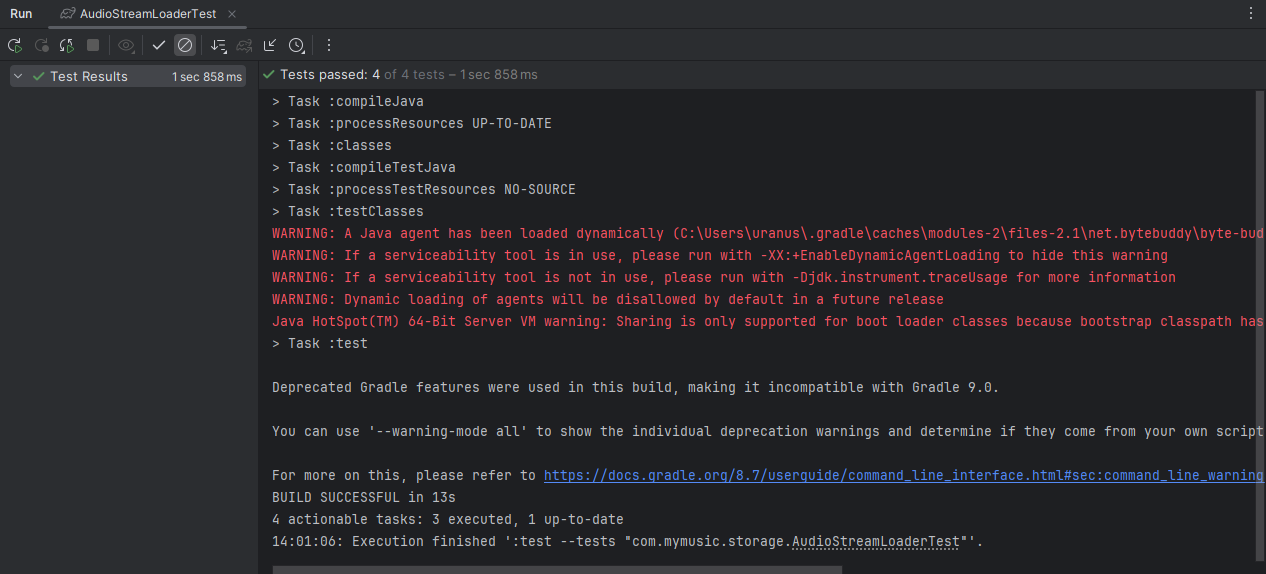
\includegraphics[width=0.8\linewidth]{unitASLSuc}}
	\caption{Результат успешного прохождения тестов для класса AudioStreamLoaer}
	\label{unitASLSuc:image}
\end{figure}
На рисунках \ref{unitJwt:image}-\ref{unitJwtvalid:image} представлены листинги модульныех тестов для модуля генерации Jwt токенов JwtTokenProvider.
\begin{figure}[!ht]
	\begin{lstlisting}[language=Java]
		class JwtTokenProviderTest {
			@Mock
			private User user;
			@Mock
			private CustomUserDetails userDetails;
			private JwtTokenProvider jwtTokenProvider;
			private final String SECRET = "mysecretkeymysecretkeymysecretkeymysecretkey";
			private final long ACCESS_EXPIRATION_IN_SEC = 3600;
			private final long REFRESH_EXPIRATION_IN_SEC = 86400;
			@BeforeEach
			void setUp() {
				MockitoAnnotations.openMocks(this);
				jwtTokenProvider = new JwtTokenProvider(SECRET, ACCESS_EXPIRATION_IN_SEC, REFRESH_EXPIRATION_IN_SEC);
			}
			@Test
			void generateAccessToken_ShouldGenerateValidToken() {
				when(user.getUserId()).thenReturn(1L);
				when(user.getRole()).thenReturn("USER");
				String token = jwtTokenProvider.generateAccessToken(user);
				assertNotNull(token);
				Claims claims = Jwts.parserBuilder().setSigningKey(SECRET).build().parseClaimsJws(token).getBody();
				assertEquals("1", claims.getSubject());
				assertEquals("USER", claims.get("ROLE"));
			}
			// Другие тесты	
		}
	\end{lstlisting}  
	\caption{Настройка и модульный тест generateAccessToken\_ShouldGenerateValidToken() класса JwtTokenProvider}
	\label{unitJwt:image}
\end{figure}
\begin{figure}[!ht]
	\begin{lstlisting}[language=Java]
		@Test
		void generateRefreshToken_ShouldGenerateValidToken() {
			when(user.getUserId()).thenReturn(1L);
			when(user.getRole()).thenReturn("USER");
			String token = jwtTokenProvider.generateRefreshToken(user);
			assertNotNull(token);
			Claims claims = Jwts.parserBuilder().setSigningKey(SECRET).build().parseClaimsJws(token).getBody();
			assertEquals("1", claims.getSubject());
			assertEquals("USER", claims.get("ROLE"));
		}
	\end{lstlisting}  
	\caption{Модульный тест generateRefreshToken\_ShouldGenerateValidToken() класса JwtTokenProvider}
	\label{unitJwtRef:image}
\end{figure}
\begin{figure}[!ht]
	\begin{lstlisting}[language=Java]
@Test
void generateRefreshToken_ShouldGenerateValidToken() {
	when(user.getUserId()).thenReturn(1L);
	when(user.getRole()).thenReturn("USER");
	String token = jwtTokenProvider.generateRefreshToken(user);
	assertNotNull(token);
	Claims claims = Jwts.parserBuilder().setSigningKey(SECRET).build().parseClaimsJws(token).getBody();
	assertEquals("1", claims.getSubject());
	assertEquals("USER", claims.get("ROLE"));
}
	\end{lstlisting}  
	\caption{Модульный тест generateRefreshToken\_ShouldGenerateValidToken() класса JwtTokenProvider}
	\label{unitJwtRef:image}
\end{figure}
\begin{figure}[!ht]
	\begin{lstlisting}[language=Java]
@Test
void isValid_ShouldReturnTrueForValidToken() {
	when(user.getUserId()).thenReturn(1L);
	when(user.getRole()).thenReturn("ROLE_USER");
	String token = jwtTokenProvider.generateAccessToken(user);	
	assertTrue(jwtTokenProvider.isValid(token, user));
}
	\end{lstlisting}  
	\caption{Модульный тест isValid\_ShouldReturnTrueForValidToken() класса JwtTokenProvider}
	\label{unitJwtvalid:image}
\end{figure}
\begin{figure}[!ht]
	\begin{lstlisting}[language=Java]
		@Test
		void isValid_ShouldReturnFalseForInvalidToken() {
			when(userDetails.getUser()).thenReturn(user);
			when(user.getUserId()).thenReturn(1L);	
			String token = "invalid.token.here";	
			assertFalse(jwtTokenProvider.isValid(token, user));
		}
	\end{lstlisting}  
\caption{Модульный тест isValid\_ShouldReturnFalseForInvalidToken() класса JwtTokenProvider}
\label{unitJwtinvalid:image}
\end{figure}
\\
Результаты успешного выполнения тестов для класса JwtTokenProvider представлены на рисунке \ref{unitJwtSuc:image}.
\begin{figure}[!ht]
	\center{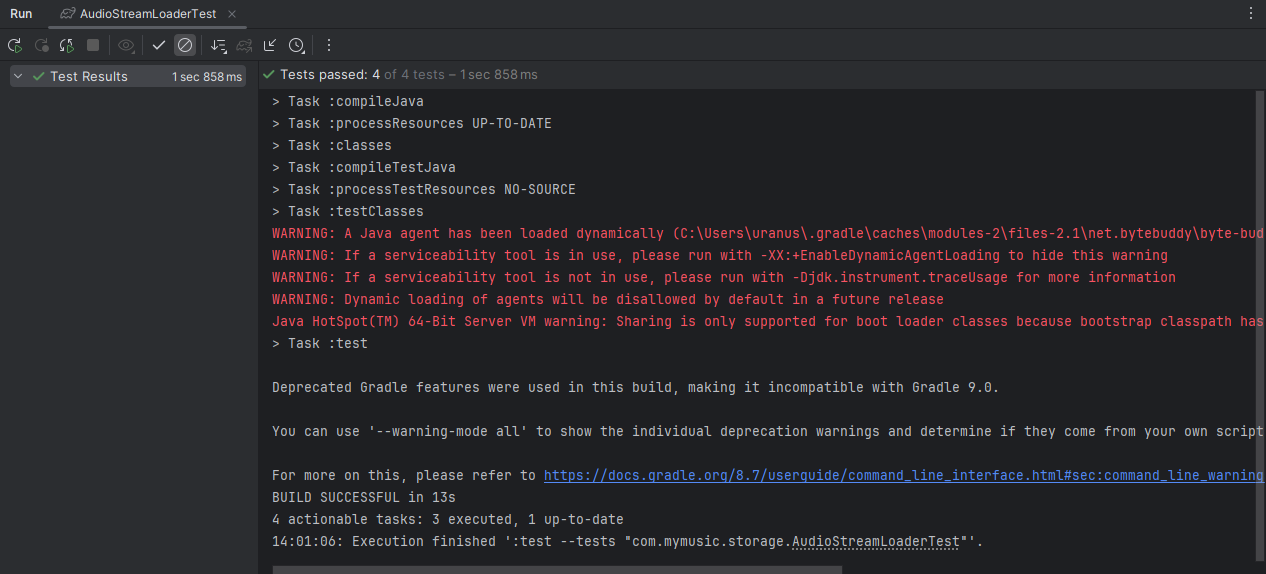
\includegraphics[width=0.7\linewidth]{unitASLSuc}}
	\caption{Результат успешного прохождения тестов для класса JwtTokenProvider}
	\label{unitJwtSuc:image}
\end{figure}


\subsubsection{Системное тестирование}

Системное тестирование является типом тестирования программного обеспечения, направленным на проверку полной интегрированной системы. На этом этапе тестируется вся система в целом, чтобы удостовериться, что все компоненты и модули работают вместе согласно требованиям спецификации. В отличие от модульного тестирования, которое фокусируется на отдельных частях программы, системное тестирование проверяет взаимодействие между различными компонентами и оценивает поведение системы в реальных условиях эксплуатации.
Системное тестирование проводится в среде, максимально приближенной к реальной эксплуатационной среде, что позволяет выявить проблемы, которые могут возникнуть в процессе использования программного обеспечения конечными пользователями.
При входе в web-приложение неаутентифицированного пользователя, ему предлагается войти в систему. Система в данном состоянии представлена на рисунке \ref{stestLoginEmpty:image}.
\begin{figure}[H]
\center{
\includegraphics[width=0.8\linewidth]{stestLoginEmpty}}
\caption{Система в состоянии "<Пользователь не аутентифицирован">}
\label{stestLoginEmpty:image}
\end{figure}
В случае наличия аутентификационных данных, пользователь может выполнить вход в систему. В случае отсутствия аутентификационных данных пользователь может перейти на страницу регистрации. Система в состоянии "<Регистрация пользователя"> представлена на рисунке \ref{stestReg:image}.
\begin{figure}[H]
	\center{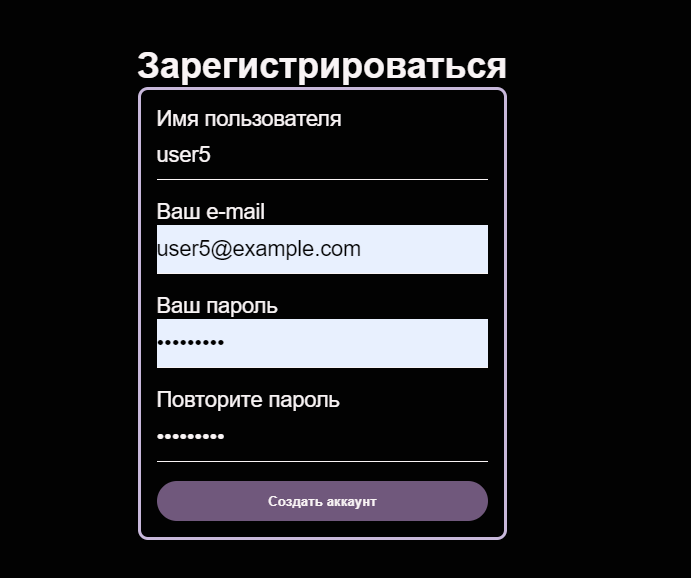
\includegraphics[width=0.8\linewidth]{stestReg}}
	\caption{Система в состоянии "<Регистрация пользователя">}
	\label{stestReg:image}
\end{figure}
После успешной регистрации пользователь вновь попадает на страницу входа, где успешно проходит аутенификацию. После этого пользователь попадает на главную страницу сайта. Данное состояние продемонстрировано на рисунке \ref{stestHome:image}.
\begin{figure}[!htb]
	\center{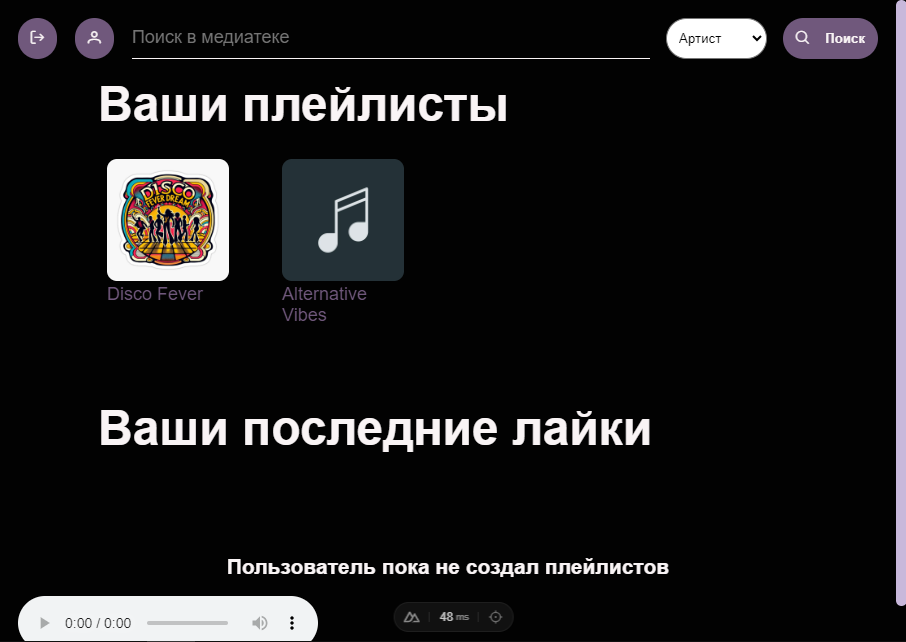
\includegraphics[width=0.8\linewidth]{stestHome}}
	\caption{Система в состоянии "<Главная страница">}
	\label{stestHome:image}
\end{figure}
Пользователь может осуществить поиск контента по строке в одной из категорий: "<артист">, "<альбом"> и "<плейлист">. В случае наличия контента пользователь получит список ссылок. Если же запрашиваемый контент не найден, то пользователь видит соответствующее сообщение. Система в состоянии "Успешный поиск" представлена на рисунке \ref{stestSearchSuc:image}.
\begin{figure}[H]
	\center{
\includegraphics[width=1\linewidth]{stestSearchSuc}}
	\caption{Система в состоянии "<Успешный поиск">}
	\label{stestSearchSuc:image}
\end{figure}
Система в состоянии "<Неудачный поиск"> представлена на рисунке \ref{stestSearchFail:image}.
\begin{figure}[H]
	\center{
\includegraphics[width=0.9\linewidth]{stestSearchFail}}
	\caption{Система в состоянии "<Неудачный поиск">}
	\label{stestSearchFail:image}
\end{figure}
В случае успешного поиска пользователь может перейти по ссылкам результата поиска. В этом случае пользователь попадает на страницу с контентом, например на страницу артиста. Система в этом состоянии представлена на рисунке \ref{stestArtist:image}.
\begin{figure}[H]
	\center{
\includegraphics[width=0.8\linewidth]{stestArtist}}
	\caption{Система в состоянии "<Страница артиста">}
	\label{stestArtist:image}
\end{figure}
Пользователь может перейти к одному из альбомов артиста, кликнув по имени альбома. В этом случае пользователь попадает на страницу альбома. Система в этом состоянии представлена на рисунке \ref{stestAlbum:image}.
\begin{figure}[H]
	\center{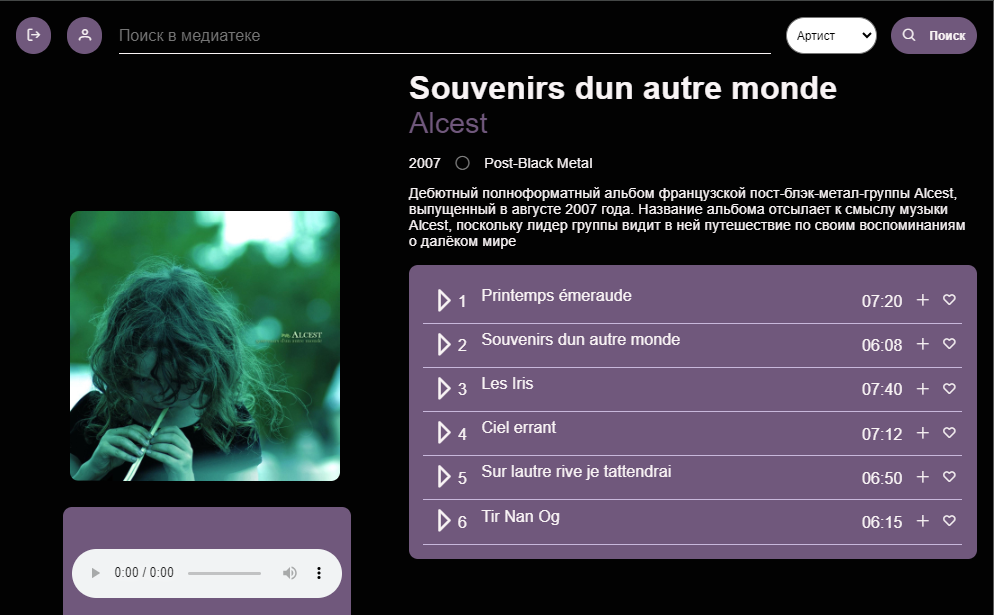
\includegraphics[width=0.8\linewidth]{stestAlbum}}
	\caption{Система в состоянии "<Страница альбома">}
	\label{stestAlbum:image}
\end{figure}
Пользователь может воспроизвести трек, щелкнув по иконке "<играть">. В этом случае плеер внизу экрана отобразит данные трека и начнется воспроизведение трека. Система в этом состоянии отображена на рисунке \ref{stestPlayer:image}.
\begin{figure}[H]
	\center{
\includegraphics[width=0.8\linewidth]{stestPlayer}}
	\caption{Система в состоянии "<Воспроизведение  трека">}
	\label{stestPlayer:image}
\end{figure}
Пользователь может получить доступ к своей странице. Для этого ему необходимо щелкнуть по кнопке с иконкой пользователя в верхней части приложения. В этом случае откроется страница пользователя. Система в этом состоянии изображена на рисунке \ref{stestUserBefore:image}.
\begin{figure}[H]
	\center{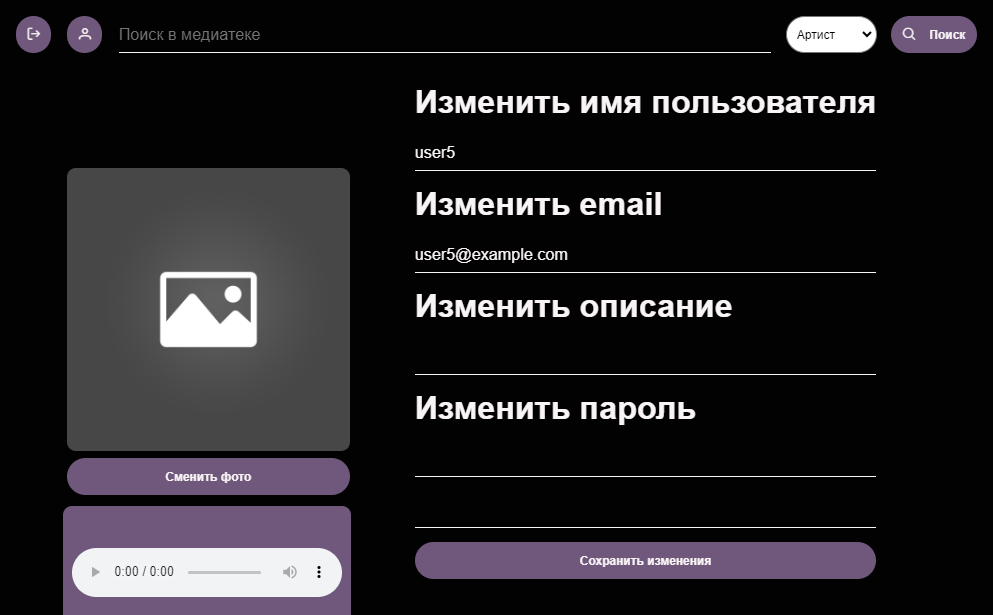
\includegraphics[width=0.8\linewidth]{stestUserBefore}}
	\caption{Система в состоянии "<Страница пользователя">}
	\label{stestUserBefore:image}
\end{figure}
Пользователь может получить изменить данные на своей странице. Для этого ему необходимо ввести новые данные в форме на странице, а затем подтвердить изменения, нажав на кнопку "<Сохранить изменения">. Система в этом состоянии изображена на рисунке \ref{stestUserAfter:image}.
\begin{figure}[H]
	\center{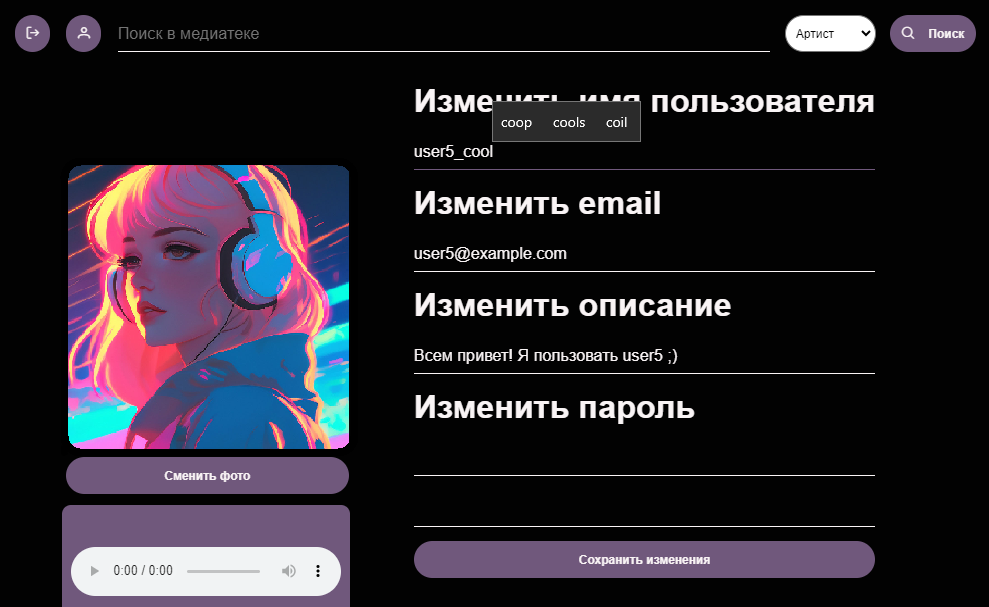
\includegraphics[width=0.8\linewidth]{stestUserAfter}}
	\caption{Система в состоянии "<Изменение данных">}
	\label{stestUserAfter:image}
\end{figure}
\clearpage
   \section*{ЗАКЛЮЧЕНИЕ}
\addcontentsline{toc}{section}{ЗАКЛЮЧЕНИЕ}
В ходе выполнения работы была спроектирована и разработана программная система, позволяющая пользователям прослушивать музыку. Также пользователям предоставлена возможность создавать плейлисты и отмечать понравившиеся треки.
Основные результаты:
\begin{enumerate}
	\item Проведен анализ предметной области; определены ключевые особенности предметной области и перспективы программного проекта.
	\item Разработана модель данных прграммной системы; определены ключевые сущности; разработан проект базы данных.
	\item Спроектированы клиентская и серверная часть программной системы; на основе требований пользователей спроектирован пользовательский интерфейс.
	\item Произведено системное тестирование системы; написаны модульные тесты.
\end{enumerate}

Все требования, описанные в техническом задании, были реализованы, все задачи, поставленные в начале разработки проекта, были также решены.

Дальнейшее развитие программной системы предполагает доработку и оптимизацию уже реализованных модулей, а также расширение возможностей приложения путем добавления системы персональных рекомендаций и интеграция с социальными сетями.
}\fi
\addcontentsline{toc}{section}{СПИСОК ИСПОЛЬЗОВАННЫХ ИСТОЧНИКОВ}

\begin{thebibliography}{9}
    \bibitem{mus1} А.А. Ивлева МУЗЫКАЛЬНЫЕ СТРИМИНГОВЫЕ СЕРВИСЫ КАК НОВЫЙ ИНСТРУМЕНТ ПРОДВИЖЕНИЯ БРЕНДОВ // Экономика и бизнес: теория и практика. 2021. №9-1. URL: https://cyberleninka.ru/article/n/muzykalnye-strimingovye-servisy-kak-novyy-instrument-prodvizheniya-brendov (дата обращения: 14.05.2024).
	\bibitem{mus2} Миннебаева Р.А., Миннебаев Р.А. АНАЛИЗ РЫНКА СТРИМИНГОВЫХ СЕРВИСОВ // Форум молодых ученых. 2018. №5-2 (21). URL: https://cyberleninka.ru/article/n/analiz-rynka-strimingovyh-servisov (дата обращения: 14.05.2024).
	\bibitem{ifpi} IFPI issues Global Music Report 2021 // IFPI URL: https://www.ifpi.org/ifpi-issues-annual-global-music-report-2021/ (дата обращения: 12.05.2024).
    \bibitem{springboot}  Уоллс К. Spring в действии. 6-е изд./ пер. с англ.А. Н. Киселева. – М.: ДМКПресс, 2022. – 544 с. - ISBN 978-5-93700-112-2. - Текст : непосредственный.
    \bibitem{springcloud} Джон Карнелл, Иллари Уайлупо Санчес Микросервисы Spring в действии / пер. с англ. А. Н. Киселева. – М.: ДМК Пресс, 2022. – 490 с. - ISBN 978-5-97060-971-2. - Текст : непосредственный.
    \bibitem{java} Шилдт Герберт Java полное руководство / Герберт Шилдт. – М : ООО "И.Д. Вильяме", 2015. – 1376 с. - ISBN 978-5-84-591759-1. - Текст : непосредственный.
    \bibitem{jshtml} Коэн Исси , Лазаро; Исси Коэн, Джозеф. А.О. Полный справочник по HTML, CSS и JavaScript / А.О. Коэн Исси , Лазаро; Исси Коэн, Джозеф.. – Паблишерз : Эксмо, 2017. – 246 с. - ISBN 978-5-9790-0009-1. - Текст : непосредственный.
    \bibitem{js} Хорстманн, К. Современный JavaScript для нетерпеливых / К. Хорстманн ; перевод с английского А. А. Слинкина. — Москва : ДМК Пресс, 2021. — 288 с. — ISBN 978-5-97060-177-8. — Текст : электронный // Лань : электронно-библиотечная система. — URL: https://e.lanbook.com/book/190715 (дата обращения: 15.05.2024). — Режим доступа: для авториз. пользователей.
    \bibitem{vue} Vue.js. Guide: Introduction to Vue.js [Электронный ресурс]. URL: https://vuejs.org/guide/introduction.html (дата обращения: 26.04.2024).
    \bibitem{ui} Мандел, Т. Разработка пользовательского интерфейса / Т. Мандел. – ДМК Пресс, 2019. – 420 с. – ISBN 978-5-04-195060-6. – Текст : непосредственный.
    \bibitem{ui2} Купер А., Рейман Р., Кронин Д., Носсел К. Интерфейс. Основы проектирования взаимодействия : [Текст] / А. Купер, Р. Рейман, Д. Кронин, К. Носсел ; пер. с англ. – 4-е изд. – СПб. : Питер, 2021. – 720 с. – ISBN 978-5-4461-0877-0. - Текст : непосредственный.
    \bibitem{arch1} Назаров, С.В. Архитектура и проектирование программных систем: монография / С.В. Назаров. – Москва : Инфра-М, 2016. – 374 с. - ISBN 978-5-16-011753-9. – Текст : непосредственный.
    \bibitem{arch2} Кугушева Дарья Сергеевна Проектирование сложного программного обеспечения с использованием микросервисной архитектуры // Инновации и инвестиции. 2020. №5. URL: https://cyberleninka.ru/article/n/proektirovanie-slozhnogo-programmnogo-obespecheniya-s-ispolzovaniem-mikroservisnoy-arhitektury (дата обращения: 27.04.2024).
    \bibitem{persist} Бауэр К., Кинг Г. Java Persistence API и Hibernate/ К. Бауэр, Г. Кинг. – Москва : ДМК Пресс, 2018. – 632 с. – ISBN 978-5-97060-674-2. – Текст : непосредственный.
    \bibitem{sql1} Грофф Д. Р. SQL. Полное руководство / Д. Р. Грофф, П. Н. Вайнберг, Э. Д. Опель. – 3-е изд.. – СПб. : Диалектика, 2019. – 560 с. - ISBN 978-5-90-711426-5 - Текст : непосредственный
    \bibitem{nosql} Григорьев, Ю.А. Реляционные базы данных и системы NoSQL: учебное пособие / Ю.А. Григорьев, А.Д. Плутенко, О.Ю. Плужникова. – Благовещенск : Амурский гос. ун-т, 2018. – 424 с. - ISBN 978-5-93493-308-2. - Текст : непосредственный.
    \bibitem{spoti} Web API | Spotify for Developers // Spotify for Developers URL: https://developer.spotify.com/documentation/web-api (дата обращения: 30.04.2024).
    \bibitem{uml} Буч, Г. Введение в UML от создателей языка / Г. Буч, И. Якобсон, Д. Рамбо. – Москва : ДМК Пресс, 2015. – 498 с. – ISBN 978-5-457-43379-3. – Текст : непосредственный.
    \bibitem{uml2} Завьялов, А. В. Диаграммы UML для анализа и проектирования информационных систем : учебно-методическое пособие / А. В. Завьялов. — Москва : РТУ МИРЭА, 2021. — 65 с. — Текст : электронный // Лань : электронно-библиотечная система. — URL: https://e.lanbook.com/book/218630 (дата обращения: 05.05.2024). — Режим доступа: для авториз. пользователей.
    \bibitem{webapi} Лоре, А. Проектирование веб-API / А. Лоре. – Москва : ДМК Пресс, 2020. – 440 с. – ISBN ISBN 978-5-97060-861-6. – Текст : непосредственный.
    \bibitem{http} Поллард Б. HTTP/2 в действии/ Б. Поллард. – Москва : ДМК Пресс, 2021. – 424 с. – ISBN 978-5-97060-925-5. – Текст: непосредственный.
    
\end{thebibliography}

\ifВКР{\appendix{Представление графического материала}

Графический материал, выполненный на отдельных листах,
изображен на рисунках А.1--А.\arabic{числоПлакатов}.
\setcounter{числоПлакатов}{0}

\renewcommand{\thefigure}{А.\arabic{figure}} % шаблон номера для плакатов

\begin{landscape}

\begin{плакат}
    \includegraphics[width=0.82\linewidth]{plakat_title}
    \заголовок{Сведения о ВКРБ}
    \label{pl1:image}      
\end{плакат}

\begin{плакат}
    \includegraphics[width=0.82\linewidth]{plakat_goals}
    \заголовок{Цель и задачи разработки}
    \label{pl2:image}      
\end{плакат}

\begin{плакат}
    \includegraphics[width=0.82\linewidth]{plakat_usecase}
    \заголовок{Диаграмма вариантов использования}
    \label{pl3:image}      
\end{плакат}

\begin{плакат}
    \includegraphics[width=0.82\linewidth]{plakat_concept}
    \заголовок{Концептуальная модель данных}
    \label{pl4:image}      
\end{плакат}

\begin{плакат}
	\includegraphics[width=0.82\linewidth]{plakat_back}
	\заголовок{Диаграмма компонентов серверной части}
	\label{pl5:image}      
\end{плакат}

\begin{плакат}
	\includegraphics[width=0.82\linewidth]{plakat_map}
	\заголовок{Карта маршрутов}
	\label{pl6:image}      
\end{плакат}

\begin{плакат}
	\includegraphics[width=0.82\linewidth]{plakat_class}
	\заголовок{Диаграмма классов предметной области}
	\label{pl7:image}      
\end{плакат}

\begin{плакат}
	\includegraphics[width=0.82\linewidth]{plakat_end}
\заголовок{Заключение}
\label{pl8:image}      
\end{плакат}


\end{landscape}
}\fi
\ifПрактика{}\else{\appendix{Фрагменты исходного кода программы}

ArtistController.java
\begin{lstlisting}[language=java]
	package com.mymusic.catalog.controllers;
	
	import com.mymusic.catalog.domain.dto.album.AlbumOfArtistPreviewDto;
	import com.mymusic.catalog.domain.dto.artist.ArtistDto;
	import com.mymusic.catalog.services.AlbumService;
	import com.mymusic.catalog.services.ArtistService;
	import org.springframework.http.HttpStatus;
	import org.springframework.http.ResponseEntity;
	import org.springframework.web.bind.annotation.*;
	
	import java.util.List;
	
	@RestController
	@RequestMapping("/artists")
	@CrossOrigin()
	public class ArtistController {
		
		private final ArtistService artistService;
		private final AlbumService albumService;
		
		public ArtistController(ArtistService artistService, AlbumService albumService) {
			this.artistService = artistService;
			this.albumService = albumService;
		}
		
		@GetMapping("/{id}")
		public ResponseEntity<ArtistDto> getArtistById(@PathVariable("id") Long id) {
			return artistService.getArtistById(id)
			.map( value -> {
				return new ResponseEntity<>(value, HttpStatus.OK);
			})
			.orElseGet(() -> new ResponseEntity<>(HttpStatus.NOT_FOUND));
		}
		
		
		@GetMapping("/{id}/albums")
		public ResponseEntity<ArtistDto> getArtistAlbums(@PathVariable("id") Long id) {
			return artistService.getArtistById(id)
			.map( value -> {
				List<AlbumOfArtistPreviewDto> albums = albumService.findArtistAlbums(id);
				value.setAlbums(albums);
				return new ResponseEntity<>(value, HttpStatus.OK);
			})
			.orElseGet(() -> new ResponseEntity<>(HttpStatus.NOT_FOUND));
		}
	}
	
\end{lstlisting}

AlbumController.java
\begin{lstlisting}[language=java]
	package com.mymusic.catalog.controllers;
	
	import com.mymusic.catalog.domain.dto.album.AlbumDto;
	import com.mymusic.catalog.mappers.AlbumMapper;
	import com.mymusic.catalog.services.AlbumService;
	import com.mymusic.catalog.services.TrackService;
	import org.springframework.http.HttpStatus;
	import org.springframework.http.ResponseEntity;
	import org.springframework.web.bind.annotation.*;
	
	@RestController
	@RequestMapping("/albums")
	@CrossOrigin()
	public class AlbumController {
		
		private final AlbumService albumService;
		private final TrackService trackService;
		
		public AlbumController(AlbumService albumService, TrackService trackService) {
			this.albumService = albumService;
			this.trackService = trackService;
		}
		
		@GetMapping("/{id}")
		public ResponseEntity<AlbumDto> getAlbumById(@PathVariable("id") Long id) {
			return albumService.findAlbumById(id)
			.map(value -> {
				AlbumDto albumDto = AlbumMapper.INSTANCE.toAlbumDto(value);
				albumDto.setTracks(trackService.getTracksInAlbum(value.getId()));
				return new ResponseEntity<>(albumDto, HttpStatus.OK);
			})
			.orElseGet(() -> new ResponseEntity<>(HttpStatus.NOT_FOUND));
		}
	}	
\end{lstlisting}

PlaylistController.java
\begin{lstlisting}[language=java]
package com.mymusic.catalog.controllers;

import com.mymusic.catalog.domain.dto.playlist.*;
import com.mymusic.catalog.domain.dto.track.PlaylistTrackModifyDto;
import com.mymusic.catalog.exceptions.ResourceNotFoundException;
import com.mymusic.catalog.services.PlaylistService;
import com.mymusic.catalog.util.HeaderStorage;
import lombok.RequiredArgsConstructor;
import org.springframework.http.HttpStatus;
import org.springframework.http.ResponseEntity;
import org.springframework.web.bind.annotation.*;

import java.util.List;

@RestController
@RequestMapping("/playlists")
@RequiredArgsConstructor
public class PlaylistController {
	
	private final PlaylistService playlistService;
	
	@GetMapping(path = "/{id}", produces = "application/json")
	public ResponseEntity<PlaylistDetailsDto> getPlaylistInfo(@PathVariable("id") Long id) {
		try {
			return ResponseEntity.ok(playlistService.getPlaylistInfoById(id));
		} catch (IllegalStateException e) {
			return ResponseEntity.internalServerError().build();
		} catch (ResourceNotFoundException e) {
			return ResponseEntity.notFound().build();
		}
	}
	
	@GetMapping(path = "/{id}/tracks")
	public ResponseEntity<PlaylistTracklistDto> getPlaylistTracklist(@PathVariable("id") Long id) {
		return ResponseEntity.ok(playlistService.getPlaylistTracklist(id));
	}
	
	@GetMapping()
	public ResponseEntity<List<PlaylistPreviewDto>> getUserPlaylists() {
		Long id = Long.parseLong(HeaderStorage.getMyHeader());
		
		return ResponseEntity.ok(playlistService.getPlaylistsByUserId(id));
	}
	
	@PostMapping()
	public ResponseEntity<PlaylistCreatedDto> createNewPlaylist(@RequestBody CreatePlaylistRequestDto newPlaylist) {
		try {
			Long playlistId = playlistService.createNewPlaylist(newPlaylist);
			return ResponseEntity.status(HttpStatus.CREATED).body(new PlaylistCreatedDto(playlistId));
		}
		catch (Exception e) {
			return ResponseEntity.internalServerError().build();
		}
	}
	
	@DeleteMapping("/{id}")
	public ResponseEntity<?> deletePlaylist(@PathVariable Long id) {
		try {
			playlistService.removePlaylistById(id);
			return ResponseEntity.ok().build();
		}
		catch (Exception e) {
			return ResponseEntity.notFound().build();
		}
	}
	
	@PostMapping(path = "/{id}/tracks")
	public ResponseEntity<?> addTracksToPlaylist(
	@RequestBody PlaylistTrackModifyDto tracks,
	@PathVariable Long id
	) {
		try {
			PlaylistTracklistDto tracklist = playlistService.addTracksToPlaylist(id, tracks.getTrackIds());
			return ResponseEntity.ok(tracklist);
		}
		catch (Exception e) {
			return ResponseEntity.notFound().build();
		}
	}
	
	@DeleteMapping(path = "/{id}/tracks")
	public ResponseEntity<PlaylistTracklistDto> removeTracksFromPlaylist(
	@RequestBody PlaylistTrackModifyDto tracks,
	@PathVariable("id") Long id
	) {
		try {
			PlaylistTracklistDto tracklist = playlistService.removeTracksFromPlaylist(id, tracks.getTrackIds());
			return ResponseEntity.ok(tracklist);
		}
		catch (Exception e) {
			return ResponseEntity.notFound().build();
		}
	}
	
}

\end{lstlisting}

SearchController.java
\begin{lstlisting}[language=java]
	package com.mymusic.catalog.controllers;
	
	import com.mymusic.catalog.domain.dto.response.BooleanResponse;
	import com.mymusic.catalog.domain.dto.track.TrackInfoDto;
	import com.mymusic.catalog.services.TrackService;
	import org.springframework.http.ResponseEntity;
	import org.springframework.web.bind.annotation.GetMapping;
	import org.springframework.web.bind.annotation.PathVariable;
	import org.springframework.web.bind.annotation.RequestMapping;
	import org.springframework.web.bind.annotation.RestController;
	
	@RestController
	@RequestMapping("/tracks")
	public class TrackController {
		
		private final TrackService trackService;
		
		public TrackController(TrackService trackService) {
			this.trackService = trackService;
		}
		
		@GetMapping("/{id}/exists")
		public ResponseEntity<BooleanResponse> isTrackExists(@PathVariable Long id) {
			return ResponseEntity.ok().body(
			trackService.isTrackExists(id)
			);
		}
		
		@GetMapping("/{id}/info")
		public ResponseEntity<TrackInfoDto> getTrackInfo(@PathVariable("id") Long id) {
			return trackService.getTrackInfo(id)
			.map(ResponseEntity::ok)
			.orElse(ResponseEntity.notFound().build());
		}
	}
\end{lstlisting}

ArtistService.java
\begin{lstlisting}[language=java]
	package com.mymusic.catalog.services;
	
	import com.mymusic.catalog.domain.dto.artist.ArtistDto;
	import com.mymusic.catalog.domain.dto.artist.ArtistPreviewDto;
	import com.mymusic.catalog.mappers.AlbumMapper;
	import com.mymusic.catalog.mappers.ArtistMapper;
	import com.mymusic.catalog.repos.ArtistsRepository;
	import org.springframework.stereotype.Service;
	
	import java.util.List;
	import java.util.Optional;
	
	@Service
	public class ArtistService {
		
		private final ArtistsRepository artistsRepository;
		
		public ArtistService(ArtistsRepository artistsRepository) {
			this.artistsRepository = artistsRepository;
		}
		
		public List<ArtistPreviewDto> getArtistsByName(String name) {
			return artistsRepository.findByNameContaining(name)
			.stream().map(artist -> {
				return ArtistMapper.INSTANCE.artistToArtistPreviewDto(artist);
			}).toList();
		}
		
		public Optional<ArtistDto> getArtistById(Long id) {
			return artistsRepository.findById(id)
			.map(artist -> {
				ArtistDto artistDto = new ArtistDto();
				artistDto.setId(artist.getId());
				artistDto.setName(artist.getName());
				artistDto.setBio(artist.getBio());
				artistDto.setImageUrl(artist.getImageUrl());
				artistDto.setAlbums(AlbumMapper.INSTANCE.albumsToAlbumOfArtistPreviewDtos(artist.getAlbums()));
				return artistDto;
			});
		}
		
		public Optional<ArtistDto> getArtistWithAlbums(Long id) {
			return artistsRepository.findById(id)
			.map(artist -> {
				ArtistDto artistDto = ArtistMapper.INSTANCE.artistToArtistDto(artist);
				artistDto.setId(artist.getId());
				return artistDto;
			});
		}
	}
	
\end{lstlisting}

AlbumService.java
\begin{lstlisting}[language=java]
	package com.mymusic.catalog.services;
	
	import com.mymusic.catalog.domain.dto.album.AlbumOfArtistPreviewDto;
	import com.mymusic.catalog.domain.entities.Album;
	import com.mymusic.catalog.mappers.AlbumMapper;
	import com.mymusic.catalog.repos.AlbumRepository;
	import jakarta.transaction.Transactional;
	import org.springframework.stereotype.Service;
	
	import java.util.List;
	import java.util.Optional;
	
	@Service
	@Transactional
	public class AlbumService {
		
		private final AlbumRepository albumRepository;
		
		public AlbumService(AlbumRepository albumRepository) {
			this.albumRepository = albumRepository;
		}
		
		public Optional<Album> findAlbumById(Long id) {
			return albumRepository.findById(id);
		}
		
		public List<AlbumOfArtistPreviewDto> findArtistAlbums(Long artistId) {
			return albumRepository.findAlbumsByArtistId(artistId)
			.stream().map(AlbumMapper.INSTANCE::albumToAlbumOfArtistPreviewDto)
			.toList();
		}
		
	}
	
\end{lstlisting}

PlaylistService.java
\begin{lstlisting}[language=java]
	package com.mymusic.catalog.services;
	
	import com.mymusic.catalog.clients.UserManagementClient;
	import com.mymusic.catalog.domain.dto.owner.OwnerPreviewDto;
	import com.mymusic.catalog.domain.dto.playlist.*;
	import com.mymusic.catalog.domain.dto.track.TrackPreviewInPlaylistDto;
	import com.mymusic.catalog.domain.entities.Playlist;
	import com.mymusic.catalog.exceptions.PlaylistNotFoundException;
	import com.mymusic.catalog.exceptions.UserNotFoundException;
	import com.mymusic.catalog.mappers.PlaylistMapper;
	import com.mymusic.catalog.repos.PlaylistRepository;
	import com.mymusic.catalog.domain.entities.Track;
	import lombok.RequiredArgsConstructor;
	import org.slf4j.Logger;
	import org.slf4j.LoggerFactory;
	import org.springframework.stereotype.Service;
	
	import java.util.*;
	
	@Service
	@RequiredArgsConstructor
	public class PlaylistService {
		
		private final Logger LOGGER = LoggerFactory.getLogger(PlaylistService.class);
		
		private final PlaylistRepository playlistRepository;
		private final TrackService trackService;
		//private final LikesClient likesClient;
		private final UserManagementClient userManagementClient;
		
		public List<PlaylistPreviewDto> getPlaylistsByUserId(Long id) {
			var l =  playlistRepository.getPlaylistsByUserId(id);
			var pl = l.stream().map(playlist -> {
				LOGGER.debug(playlist.getName());
				return new PlaylistPreviewDto(
				playlist.getId(),
				playlist.getName(),
				playlist.getCoverUrl()
				);
			}).toList();
			
			return pl;
		}
		
		public Set<Track> getTracksByPlaylistId(long playlistId) {
			return playlistRepository.findTracksByPlaylistId(playlistId)
			.orElse(Collections.emptySet());
		}
		
		public Optional<Playlist> getPlaylistById(long playlistId) {
			return playlistRepository.findById(playlistId);
		}
		
		public Long createNewPlaylist(CreatePlaylistRequestDto newPlaylist) throws Exception {
			var userExists = userManagementClient
			.isUserExists(newPlaylist.getOwnerId());
			
			if (!userExists.isExists()) {
				throw new UserNotFoundException(newPlaylist.getOwnerId());
			}
			
			Playlist playlist = new Playlist();
			
			playlist.setName(newPlaylist.getName());
			playlist.setDescription(newPlaylist.getDescription());
			playlist.setCoverUrl(newPlaylist.getCover());
			playlist.setUserId(newPlaylist.getOwnerId());
			
			playlist = playlistRepository.save(playlist);
			addTracksToPlaylist(playlist.getId(), newPlaylist.getTrackIds());
			
			return playlist.getId();
		}
		
		public void removePlaylistById(Long id) throws Exception {
			Playlist playlist = playlistRepository.findPlaylistById(id)
			.orElseThrow(() -> new Exception("Playlist not found"));
			
			playlistRepository.delete(playlist);
		}
		
		public Optional<PlaylistDto> getPlaylistDtoById(Long id) {
			
			Optional<Playlist> playlistOptional = playlistRepository.findPlaylistById(id);
			
			return playlistOptional.map(playlist -> {
				PlaylistDto playlistDto = new PlaylistDto();
				playlistDto.setId(playlist.getId());
				playlistDto.setName(playlist.getName());
				playlistDto.setDescription(playlist.getDescription());
				playlistDto.setUserId(playlist.getUserId());
				playlistDto.setCoverUrl(playlist.getCoverUrl());
				
				Optional<List<TrackPreviewInPlaylistDto>> tracklistOptional = trackService.getTracksWithCoverInPlaylist(id);
				List<TrackPreviewInPlaylistDto> tracks = tracklistOptional.orElseGet(ArrayList::new);
				playlistDto.setTracks(tracks);
				
				return playlistDto;
			});
		}
		
		public PlaylistTracklistDto addTracksToPlaylist(Long id, Iterable<Long> trackIds) throws Exception {
			Playlist playlist = playlistRepository.findPlaylistById(id)
			.orElseThrow(() -> new Exception("Playlist not found"));
			
			List<Track> tracks = trackService.getTracksByIds(trackIds);
			
			for (Track t : tracks) {
				playlist.addTrack(t);
			}
			
			playlist = playlistRepository.save(playlist);
			return PlaylistMapper.INSTANCE.toPlaylistTracklistDto(playlist);
		}
		
		public PlaylistTracklistDto removeTracksFromPlaylist(Long id, Iterable<Long> trackIds) throws Exception {
			Playlist playlist = playlistRepository.findPlaylistById(id)
			.orElseThrow(() -> new Exception("Playlist not found"));
			
			List<Track> tracks = trackService.getTracksByIds(trackIds);
			
			for (Track t : tracks) {
				playlist.removeTrack(t);
			}
			
			playlist = playlistRepository.save(playlist);
			return PlaylistMapper.INSTANCE.toPlaylistTracklistDto(playlist);
		}
		
		public List<PlaylistPreviewDto> getRandomPlaylistsContainingLikedTracks() {
			return null;
		}
		
		public PlaylistDetailsDto getPlaylistInfoById(Long id)
		throws IllegalStateException, PlaylistNotFoundException, UserNotFoundException {
			Playlist playlist = playlistRepository.findPlaylistById(id)
			.orElseThrow(() -> new PlaylistNotFoundException(id));
			
			OwnerPreviewDto owner = userManagementClient.getUserPreview(playlist.getUserId());
			
			PlaylistDetailsDto playlistInfo = PlaylistMapper.INSTANCE.playlistToPlaylistInfoDto(playlist);
			playlistInfo.setOwner(owner);
			
			return playlistInfo;
		}
		
		public PlaylistTracklistDto getPlaylistTracklist(Long playlistId) {
			Set<Track> tracks = playlistRepository.findTracksByPlaylistId(playlistId)
			.orElse(Collections.emptySet());
			PlaylistTracklistDto tracklist = new PlaylistTracklistDto();
			tracklist.setTracks(tracks);
			return tracklist;
		}
	}
	
\end{lstlisting}

LikeService.java
\begin{lstlisting}[language=java]
	package com.mymusic.likes.services;
	
	import com.mymusic.likes.clients.CatalogClient;
	import com.mymusic.likes.clients.UserManagerClient;
	import com.mymusic.likes.entities.Like;
	import com.mymusic.likes.repos.LikeRepository;
	import lombok.RequiredArgsConstructor;
	import org.springframework.stereotype.Service;
	
	import java.util.List;
	import java.util.Optional;
	
	@Service
	@RequiredArgsConstructor
	public class LikeService {
		
		private final LikeRepository likeRepository;
		private final UserManagerClient userManagerClient;
		private final CatalogClient catalogClient;
		
		public Optional<List<Like>> getUserLikes(Long userId) {
			if (validateUser(userId)) {
				return Optional.of(
				likeRepository.findLikeByUserId(userId));
			}
			else {
				return Optional.empty();
			}
		}
		
		public Optional<List<Like>> getTrackLikes(Long trackId) {
			if (validateTrack(trackId)) {
				return Optional.of(
				likeRepository.findLikeByUserId(trackId));
			}
			else {
				return Optional.empty();
			}
		}
		
		public boolean save(Like like) {
			if (validateUser(like.userId()) && validateTrack(like.trackId())) {
				likeRepository.save(like);
				return true;
			}
			else return false;
		}
		
		public boolean delete(Like like) {
			if (validateUser(like.userId()) && validateTrack(like.trackId())) {
				likeRepository.delete(like);
				return true;
			}
			else return false;
		}
		
	}
	
\end{lstlisting}

AudioStreamLoader.java
\begin{lstlisting}[language=java]
	package com.mymusic.storage.services;
	
	
	import com.mymusic.storage.exceptions.ResourceNotFoundException;
	import com.mymusic.storage.utils.RangeValuesUtils;
	import lombok.RequiredArgsConstructor;
	import org.slf4j.Logger;
	import org.slf4j.LoggerFactory;
	import org.springframework.stereotype.Service;
	import org.springframework.util.StringUtils;
	import org.springframework.web.servlet.mvc.method.annotation.StreamingResponseBody;
	
	import java.io.ByteArrayInputStream;
	import java.io.IOException;
	import java.io.InputStream;
	
	
	@Service
	@RequiredArgsConstructor
	public class AudioStreamLoader {
		
		private static final Logger LOGGER = LoggerFactory.getLogger(AudioStreamLoader.class);
		
		private final S3Service s3Service;
		private final RangeValuesUtils rangeValuesUtils;
		
		public record StreamingResponseResult(
		long start,
		long end,
		long filesize,
		StreamingResponseBody body
		) {
			public long getContentLength() {
				return  (end - start) + 1;
			}
		}
		
		private StreamingResponseResult loadPartialMediaFromStorage(
		byte[] bytes,
		long startPos,
		long endPos
		) throws ResourceNotFoundException, IOException {
			StreamingResponseBody responseStream;
			
			long filesize = bytes.length;
			
			if (startPos < 0L) {
				startPos = 0;
			}
			if (filesize > 0L)
			{
				if (startPos >= filesize)
				{
					startPos = filesize - 1L;
				}
				
				if (endPos >= filesize)
				{
					endPos = filesize - 1L;
				}
			}
			else
			{
				startPos = 0L;
				endPos = 0L;
			}
			byte[] buffer = new byte[1024];
			
			long finalEndPos = endPos;
			long finalStartPos = startPos;
			responseStream = outputStream -> {
				try (InputStream is = new ByteArrayInputStream(bytes)) {
					is.skip(finalStartPos);
					long pos = finalStartPos;
					int bytesRead;
					while (pos <= finalEndPos && (bytesRead = is.read(buffer, 0, (int) Math.min(buffer.length, finalEndPos - pos + 1))) != -1) {
						outputStream.write(buffer, 0, bytesRead);
						pos += bytesRead;
					}
					outputStream.flush();
				}
			};
			
			return new StreamingResponseResult(startPos, endPos, filesize, responseStream);
		}
		
		public StreamingResponseResult loadPartialMediaFromStorage(
		Long id,
		String rangeValues
		) throws ResourceNotFoundException, IOException, IllegalArgumentException {
			
			var bytes = s3Service.getTrackObject(id);
			
			if (!StringUtils.hasText(rangeValues))
			{
				return loadEntireMediaFile(bytes);
			}
			
			long fileSize = bytes.length;
			long[] ranges = rangeValuesUtils.extractRangeValues(rangeValues);
			long rangeStart = ranges[0];
			long rangeEnd = ranges[1];
			
			
			if ((rangeEnd == 0L || rangeEnd == -1L) && fileSize > 0L)
			{
				rangeEnd = fileSize - 1;
			}
			if (fileSize < rangeEnd)
			{
				rangeEnd = fileSize - 1;
			}
			
			return loadPartialMediaFromStorage(bytes, rangeStart, rangeEnd);
		}
		
		public StreamingResponseResult loadEntireMediaFile(
		byte[] bytes
		) throws IOException
		{
			long fileSize = bytes.length;
			long endPos;
			if (fileSize > 0L)
			{
				endPos = fileSize - 1;
			}
			else
			{
				endPos = 0L;
			}
			
			return loadPartialMediaFromStorage(bytes, 0, endPos);
		}
	}
\end{lstlisting}

AuthenticationController.java
\begin{lstlisting}[language=java]
	package com.mymusic.auth.controllers;
	
	import com.mymusic.auth.domain.entities.Token;
	import com.mymusic.auth.domain.requests.LoginDto;
	import com.mymusic.auth.services.AuthenticationService;
	import jakarta.servlet.http.Cookie;
	import jakarta.servlet.http.HttpServletResponse;
	import lombok.RequiredArgsConstructor;
	import org.springframework.http.HttpStatus;
	import org.springframework.http.ResponseEntity;
	import org.springframework.security.authentication.BadCredentialsException;
	import org.springframework.security.core.userdetails.UsernameNotFoundException;
	import org.springframework.web.bind.annotation.*;
	
	@RestController
	@RequiredArgsConstructor
	@RequestMapping("/auth")
	public class AuthenticationController {
		
		private final AuthenticationService authenticationService;
		
		@PostMapping("/login")
		public ResponseEntity<?> login(@RequestBody LoginDto login, HttpServletResponse response) {
			try {
				Token tokens = authenticationService.login(login.getEmail(), login.getPassword());
				response.addHeader("Authorization", "Bearer " + tokens.getAccess());
				response.addCookie(
				new Cookie("Refresh", tokens.getRefresh())
				);
				return ResponseEntity.noContent().build();
			}
			catch (UsernameNotFoundException e) {
				return ResponseEntity.notFound().build();
			}
			catch (BadCredentialsException e) {
				
				return ResponseEntity.status(HttpStatus.UNAUTHORIZED).build();
			}
			catch (Exception e) {
				return ResponseEntity.internalServerError().build();
			}
		}
		
	}
\end{lstlisting}

JwtTokenProvider.java
\begin{lstlisting}[language=java]
package com.mymusic.auth.configuration;

import com.mymusic.auth.domain.entities.User;
import io.jsonwebtoken.Claims;
import io.jsonwebtoken.Jwts;
import io.jsonwebtoken.MalformedJwtException;
import io.jsonwebtoken.io.Decoders;
import io.jsonwebtoken.security.Keys;
import lombok.Getter;
import org.springframework.beans.factory.annotation.Value;
import org.springframework.stereotype.Component;

import java.security.Key;
import java.time.Instant;
import java.util.Date;
import java.util.Objects;
import java.util.concurrent.TimeUnit;
import java.util.function.Function;

@Component
public class JwtTokenProvider {
	
	private final String SECRET;
	@Getter
	private final long ACCESS_EXPIRATION_IN_SEC;
	@Getter
	private final long REFRESH_EXPIRATION_IN_SEC;
	
	public JwtTokenProvider(
	@Value("${jwt.secret}") String secret,
	@Value("${jwt.access-expiration}") long accessExp,
	@Value("${jwt.refresh-expiration}") long refreshExp
	) {
		this.SECRET = secret;
		this.ACCESS_EXPIRATION_IN_SEC = accessExp;
		this.REFRESH_EXPIRATION_IN_SEC = refreshExp;
	}
	
	private Key getSecretKey() {
		byte[] byteKey = Decoders.BASE64.decode(this.SECRET);
		return Keys.hmacShaKeyFor(byteKey);
	}
	
	public String generateRefreshToken(User user) {
		return generateToken(user, REFRESH_EXPIRATION_IN_SEC);
	}
	
	public String generateAccessToken(User user) {
		return generateToken(user, ACCESS_EXPIRATION_IN_SEC);
	}
	
	public String generateToken(User user, Long expTime) {
		Claims claims = Jwts.claims()
		.setSubject(user.getUserId().toString());
		
		claims.put("ROLE", user.getRole());
		
		var now = Instant.now();
		claims.setIssuedAt(Date.from(now));
		claims.setExpiration(Date.from(now.plus(expTime, TimeUnit.SECONDS.toChronoUnit())));
		
		return Jwts.builder()
		.setClaims(claims)
		.signWith(getSecretKey())
		.compact();
	}
	
	private Claims extractAllClaims(String token) {
		return Jwts.parserBuilder()
		.setSigningKey(getSecretKey())
		.build()
		.parseClaimsJws(token)
		.getBody();
	}
	
	private <T> T extractClaim(String token, Function<Claims, T> claimsResolver) {
		Claims claims = extractAllClaims(token);
		return claimsResolver.apply(claims);
	}
	
	private Date extractExpiration(String token) {
		return extractClaim(token, Claims::getExpiration);
	}
	
	private Long extractUserId(String token) {
		return Long.valueOf(extractClaim(token, Claims::getSubject));
	}
	
	public boolean isValid(String token, User user) {
		try {
			Long userId = user.getUserId();
			return (Objects.equals(userId, extractUserId(token))) && isExpired(token);
		}
		catch (MalformedJwtException e) {
			return false;
		}
	}
	
	private boolean isExpired(String token) {
		var exp = extractClaim(token, Claims::getExpiration);
		var now = new Date();
		return now.before(exp);
	}
}
\end{lstlisting}
\ifВКР{
\newpage
\addcontentsline{toc}{section}{На отдельных листах (CD-RW в прикрепленном конверте)}
\begin{center}
\textbf{Место для диска}
\end{center}
}\fi
}\fi
\end{document}
